%\documentclass[11pt,a4paper,oneside]{report} % Single-side
\documentclass[11pt,a4paper,twoside,openright]{report}  % Duplex

% thanks to http://tex.stackexchange.com/a/47579/71109
\usepackage{ifxetex}
\usepackage{ifluatex}
\newif\ifxetexorluatex % a new conditional starts as false
\ifnum 0\ifxetex 1\fi\ifluatex 1\fi>0
  \xetexorluatextrue
\fi

\ifxetexorluatex
  \usepackage{fontspec}
\else
  \usepackage[T1]{fontenc}
  \usepackage[utf8]{inputenc}
  \usepackage[lighttt]{lmodern}
\fi

\usepackage[english,magyar]{babel} % Alapértelmezés szerint utoljára definiált nyelv lesz aktív, de később külön beállítjuk az aktív nyelvet.

%\usepackage{cmap}
\usepackage{amsfonts,amsmath,amssymb} % Mathematical symbols.
%\usepackage[ruled,boxed,resetcount,linesnumbered]{algorithm2e} % For pseudocodes. % beware: this is not compatible with LuaLaTeX, see http://tex.stackexchange.com/questions/34814/lualatex-and-algorithm2e
\usepackage{booktabs} % For publication quality tables for LaTeX
\usepackage{graphicx}

%\usepackage{fancyhdr}
%\usepackage{lastpage}

\usepackage{anysize}
%\usepackage{sectsty}
\usepackage{setspace} % For setting line spacing

\usepackage[unicode]{hyperref} % For hyperlinks in the generated document.
\usepackage[pdftex,dvipsnames,table]{xcolor}  % Coloured text etc.
\usepackage{listings} % For source code snippets.

\usepackage[amsmath,thmmarks]{ntheorem} % Theorem-like environments.

\usepackage[hang]{caption}

\singlespacing

\newcommand{\selecthungarian}{
  \selectlanguage{magyar}
  \setlength{\parindent}{2em}
  \setlength{\parskip}{0em}
  \frenchspacing
}

\newcommand{\selectenglish}{
  \selectlanguage{english}
  \setlength{\parindent}{0em}
  \setlength{\parskip}{0.5em}
  \nonfrenchspacing
  \renewcommand{\figureautorefname}{Figure}
  \renewcommand{\tableautorefname}{Table}
  \renewcommand{\partautorefname}{Part}
  \renewcommand{\chapterautorefname}{Chapter}
  \renewcommand{\sectionautorefname}{Section}
  \renewcommand{\subsectionautorefname}{Section}
  \renewcommand{\subsubsectionautorefname}{Section}
}

\usepackage[numbers]{natbib}
\usepackage{xspace}

% Personal
\usepackage{tikz}
\usepackage{physics} % Braket notation
\usepackage{dsfont} % Mathds
\usepackage{xargs} % Use more than one optional parameter in a new commands
\usepackage[colorinlistoftodos,prependcaption,textsize=tiny]{todonotes} % Todo notes.
\newcommandx{\unsure}[2][1=]{\todo[inline,size=\normalsize,linecolor=red,backgroundcolor=red!25,bordercolor=red,#1]{#2}}
\newcommandx{\change}[2][1=]{\todo[inline,size=\normalsize,linecolor=blue,backgroundcolor=blue!25,bordercolor=blue,#1]{#2}}
\newcommandx{\info}[2][1=]{\todo[inline,size=\normalsize,linecolor=OliveGreen,backgroundcolor=OliveGreen!25,bordercolor=OliveGreen,#1]{#2}}

\newcommand{\vikszerzoVezeteknev}{Nemkin}
\newcommand{\vikszerzoKeresztnev}{Viktória}

\newcommand{\vikkonzulensAMegszolitas}{dr.~}
\newcommand{\vikkonzulensAVezeteknev}{Friedl}
\newcommand{\vikkonzulensAKeresztnev}{Katalin}

\newcommand{\vikcim}{Application of Quantum Computing\\in Bioinformatics}
\newcommand{\viktanszek}{\bmeszit}
\newcommand{\vikdoktipus}{\msc}
\newcommand{\vikmunkatipusat}{diplomatervet}

\newcommand{\szerzoMeta}{\vikszerzoVezeteknev{} \vikszerzoKeresztnev}

%--------------------------------------------------------------------------------------
% Elnevezések
%--------------------------------------------------------------------------------------
\newcommand{\bme}{Budapest University of Technology and Economics}
\newcommand{\vik}{Faculty of Electrical Engineering and Informatics}

\newcommand{\bmeszit}{Department of Computer Science and Information Theory}

\newcommand{\keszitette}{Author}
\newcommand{\konzulens}{Advisor}

\newcommand{\bsc}{Bachelor's Thesis}
\newcommand{\msc}{Master's Thesis}
\newcommand{\tdk}{Scientific Students' Association Report}
\newcommand{\bsconlab}{BSc Project Laboratory}
\newcommand{\msconlabi}{MSc Project Laboratory 1}
\newcommand{\msconlabii}{MSc Project Laboratory 2}

\newcommand{\pelda}{Example}
\newcommand{\definicio}{Definition}
\newcommand{\tetel}{Theorem}

\newcommand{\bevezetes}{Introduction}
\newcommand{\koszonetnyilvanitas}{Acknowledgements}
\newcommand{\fuggelek}{Appendix}

% Optional custom titles
%\addto\captionsenglish{%
%\renewcommand*{\listfigurename}{Your list of figures title}
%\renewcommand*{\listtablename}{Your list of tables title}
%\renewcommand*{\bibname}{Your bibliography title}
%}

\newcommand{\szerzo}{\vikszerzoKeresztnev{} \vikszerzoVezeteknev}
\newcommand{\vikkonzulensA}{\vikkonzulensAMegszolitas\vikkonzulensAKeresztnev{} \vikkonzulensAVezeteknev}
\newcommand{\vikkonzulensB}{\vikkonzulensBMegszolitas\vikkonzulensBKeresztnev{} \vikkonzulensBVezeteknev}
\newcommand{\vikkonzulensC}{\vikkonzulensCMegszolitas\vikkonzulensCKeresztnev{} \vikkonzulensCVezeteknev}

\newcommand{\selectthesislanguage}{\selectenglish}

\bibliographystyle{plainnat}

\newcommand{\ie}{i.e.\@\xspace}
\newcommand{\Ie}{I.e.\@\xspace}
\newcommand{\eg}{e.g.\@\xspace}
\newcommand{\Eg}{E.g.\@\xspace}
\newcommand{\etal}{et al.\@\xspace}
\newcommand{\etc}{etc.\@\xspace}
\newcommand{\vs}{vs.\@\xspace}
\newcommand{\viz}{viz.\@\xspace} % videlicet
\newcommand{\cf}{cf.\@\xspace} % confer
\newcommand{\Cf}{Cf.\@\xspace}
\newcommand{\wrt}{w.r.t.\@\xspace} % with respect to
\newcommand{\approximately}{approx.\@\xspace}

\newcommand{\appendixnumber}{1}  % a fofejezet-szamlalo az angol ABC 1. betuje (A) lesz

% Page layout setup
\pagestyle{plain}
\marginsize{35mm}{25mm}{15mm}{15mm}
\setcounter{tocdepth}{3}
\setcounter{secnumdepth}{3}

% Margón túllógó sorok tiltása.
\sloppy
% A fattyú- és árvasorok elkerülése.
\widowpenalty=10000
\clubpenalty=10000

% Kötőjeles szavak elválasztásának engedélyezése
\def\hyph{-\penalty0\hskip0pt\relax}

% Setup hyperref package
\hypersetup{
    % bookmarks=true,          % show bookmarks bar?
    unicode=true,              % non-Latin characters in Acrobat's bookmarks
    pdftitle={\vikcim},        % title
    pdfauthor={\szerzoMeta},   % author
    pdfsubject={\vikdoktipus}, % subject of the document
    pdfcreator={\szerzoMeta},  % creator of the document
    pdfproducer={},            % producer of the document
    pdfkeywords={},            % list of keywords (separate then by comma)
    pdfnewwindow=true,         % links in new window
    colorlinks=true,           % false: boxed links; true: colored links
    linkcolor=black,           % color of internal links
    citecolor=black,           % color of links to bibliography
    filecolor=black,           % color of file links
    urlcolor=black             % color of external links
}

% Set up listings
\definecolor{lightgray}{rgb}{0.95,0.95,0.95}
\lstset{
	basicstyle=\scriptsize\ttfamily, % print whole listing small
	keywordstyle=\color{black}\bfseries, % bold black keywords
	identifierstyle=, % nothing happens
	% default behavior: comments in italic, to change use
	% commentstyle=\color{green}, % for e.g. green comments
	stringstyle=\scriptsize,
	showstringspaces=false, % no special string spaces
	aboveskip=3pt,
	belowskip=3pt,
	backgroundcolor=\color{lightgray},
	columns=flexible,
	keepspaces=true,
	escapeinside={(*@}{@*)},
	captionpos=b,
	breaklines=true,
	frame=single,
	float=!ht,
	tabsize=2,
	literate=*
		{á}{{\'a}}1	{é}{{\'e}}1	{í}{{\'i}}1	{ó}{{\'o}}1	{ö}{{\"o}}1	{ő}{{\H{o}}}1	{ú}{{\'u}}1	{ü}{{\"u}}1	{ű}{{\H{u}}}1
		{Á}{{\'A}}1	{É}{{\'E}}1	{Í}{{\'I}}1	{Ó}{{\'O}}1	{Ö}{{\"O}}1	{Ő}{{\H{O}}}1	{Ú}{{\'U}}1	{Ü}{{\"U}}1	{Ű}{{\H{U}}}1
}

% Set up theorem-like environments

\theoremseparator{.}
\theorembodyfont{\upshape}
\newtheorem{example}{\pelda}
\newtheorem{property}{\tulajdonsag}
\newtheorem{definition}{\definicio}
\newtheorem{theorem}{\tetel}
\numberwithin{example}{chapter}
\numberwithin{property}{chapter}
\numberwithin{definition}{chapter}
\numberwithin{theorem}{chapter}

\newcommand{\lineparagraph}[1]{\paragraph{#1}\mbox{}\\}
\newcommand{\linesubparagraph}[1]{\subparagraph{#1}\mbox{}\\}

% Setup captions
\captionsetup[figure]{
	width=.75\textwidth,
	aboveskip=10pt}

\renewcommand{\captionlabelfont}{\bf}
\renewcommand{\captionfont}{\footnotesize\it}

% Hyphenation exceptions
\hyphenation{Shakes-peare Mar-seilles ár-víz-tű-rő tü-kör-fú-ró-gép}

\author{\vikszerzo}
\title{\viktitle}

\begin{document}

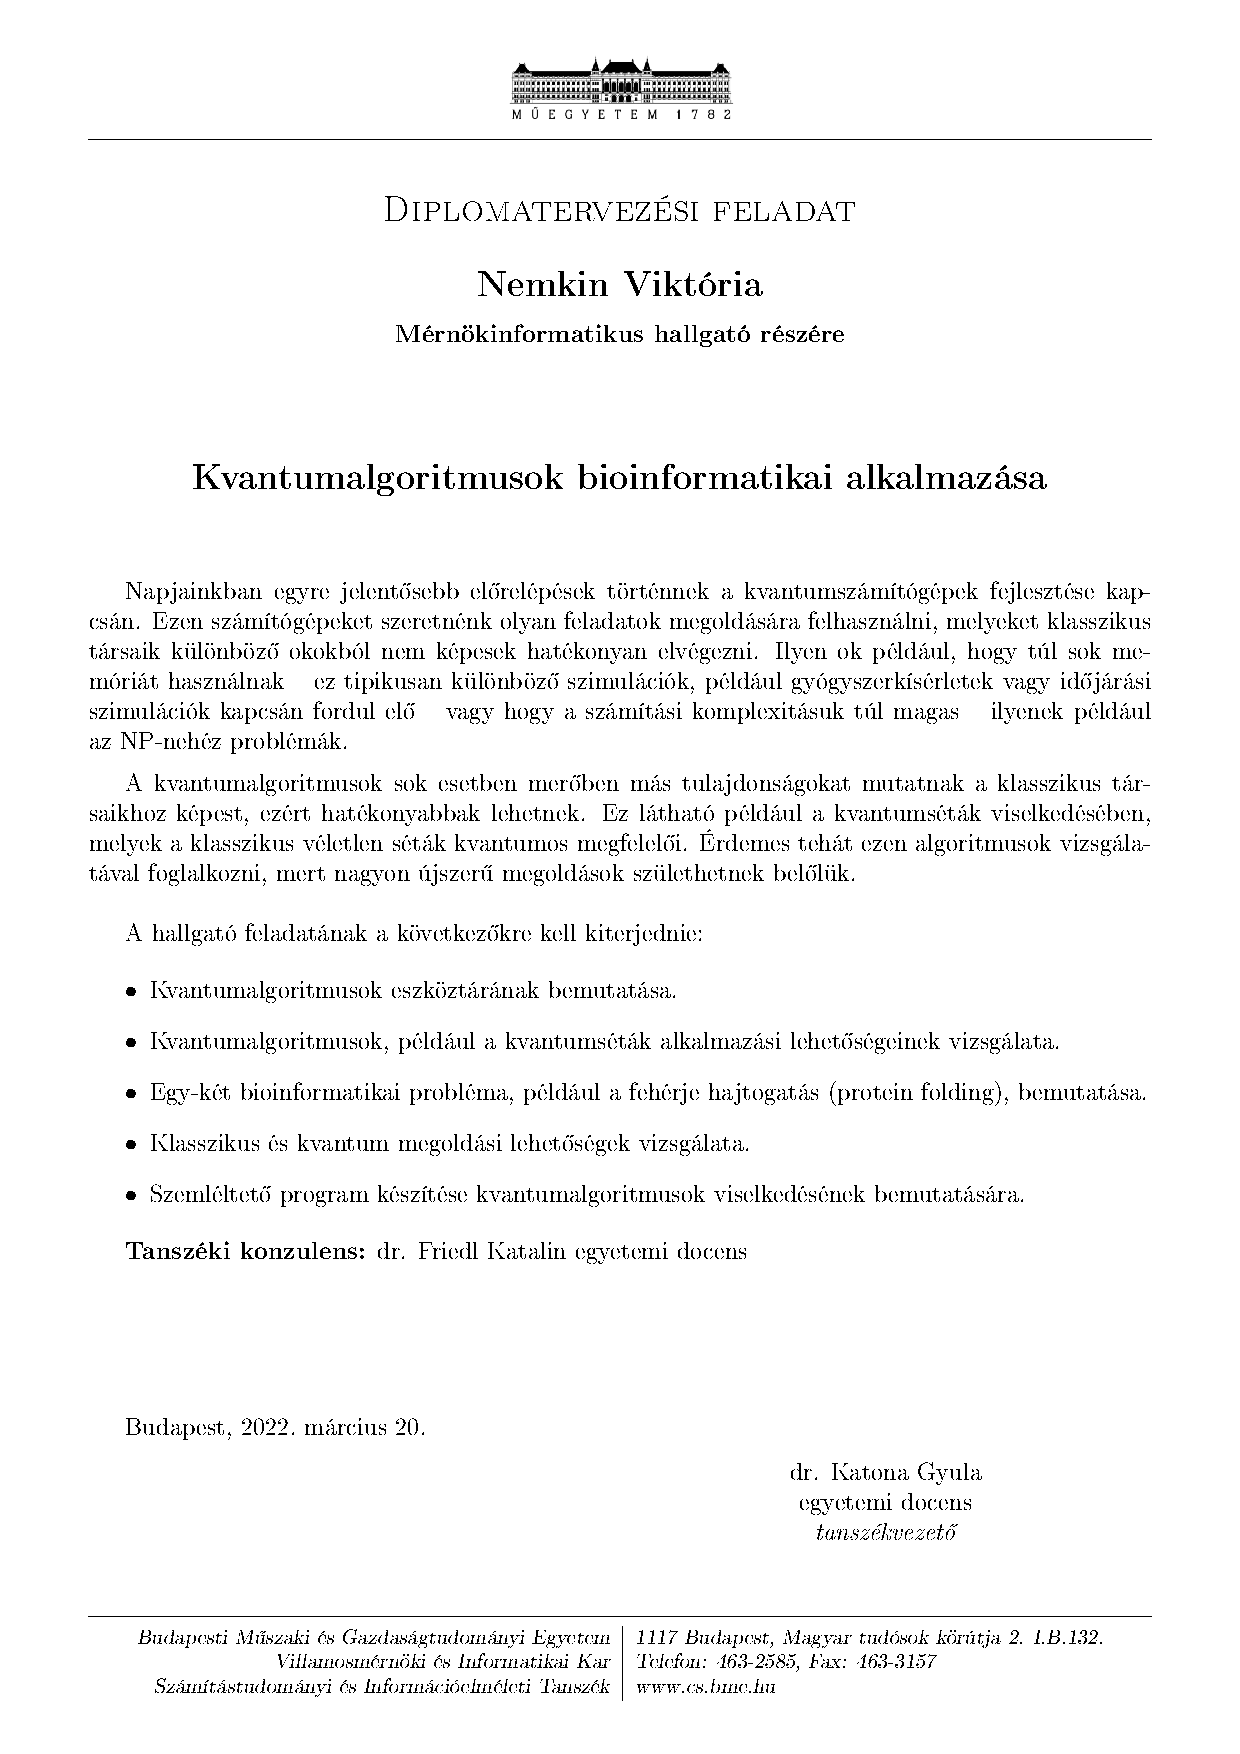
\includepdf[pages=-]{task.pdf}
\afterpage{\null\newpage}

\pagenumbering{gobble}
\selectthesislanguage
\hypersetup{pageanchor=false}
%--------------------------------------------------------------------------------------
%	The title page
%--------------------------------------------------------------------------------------
\begin{titlepage}
\begin{center}

\includegraphics[width=60mm,keepaspectratio]{figures/bme_logo.pdf}\\
\vspace{0.3cm}
\textbf{\bme}\\
\textmd{\vik}\\
\textmd{\viktanszek}\\[5cm]

\vspace{0.4cm}
{\huge \bfseries \vikcim}\\[0.8cm]
\vspace{0.5cm}
\textsc{\Large \vikdoktipus}\\[4cm]

{
	\renewcommand{\arraystretch}{0.85}
	\begin{tabular}{cc}
	 \makebox[7cm]{\emph{\keszitette}} & \makebox[7cm]{\emph{\konzulens}} \\ \noalign{\smallskip}
	 \makebox[7cm]{\szerzo} & \makebox[7cm]{\vikkonzulensA} \\
	\end{tabular}
}

\vfill
{\large December 18, 2022}
\end{center}
\end{titlepage}
\hypersetup{pageanchor=false}


\tableofcontents\vfill

\selectlanguage{magyar}
\pagenumbering{gobble}
%--------------------------------------------------------------------------------------
% Nyilatkozat
%--------------------------------------------------------------------------------------
\begin{center}
\large
\textbf{HALLGATÓI NYILATKOZAT}\\
\end{center}

Alulírott \emph{\vikszerzoVezeteknev{} \vikszerzoKeresztnev}, szigorló hallgató kijelentem, hogy ezt a \vikmunkatipusat{} meg nem engedett segítség nélkül, saját magam készítettem, csak a megadott forrásokat (szakirodalom, eszközök stb.) használtam fel. Minden olyan részt, melyet szó szerint, vagy azonos értelemben, de átfogalmazva más forrásból átvettem, egyértelműen, a forrás megadásával megjelöltem.

Hozzájárulok, hogy a jelen munkám alapadatait (szerző(k), cím, angol és magyar nyelvű tartalmi kivonat, készítés éve, konzulens(ek) neve) a BME VIK nyilvánosan hozzáférhető elektronikus formában, a munka teljes szövegét pedig az egyetem belső hálózatán keresztül (vagy autentikált felhasználók számára) közzétegye. Kijelentem, hogy a benyújtott munka és annak elektronikus verziója megegyezik. Dékáni engedéllyel titkosított diplomatervek esetén a dolgozat szövege csak 3 év eltelte után válik hozzáférhetővé.

\begin{flushleft}
\vspace*{1cm}
Budapest, \today
\end{flushleft}

\begin{flushright}
 \vspace*{1cm}
 \makebox[7cm]{\rule{6cm}{.4pt}}\\
 \makebox[7cm]{\emph{\vikszerzoVezeteknev{} \vikszerzoKeresztnev}}\\
 \makebox[7cm]{hallgató}
\end{flushright}
\thispagestyle{empty}

\vfill
\clearpage
\thispagestyle{empty} % an empty page

\selectthesislanguage

\pagenumbering{roman}
\setcounter{page}{1}

\selecthungarian

%----------------------------------------------------------------------------
% Abstract in Hungarian
%----------------------------------------------------------------------------
\chapter*{Kivonat}\addcontentsline{toc}{chapter}{Kivonat}

A bioinformatika egy interdiszciplináris terület az informatika és a biológia határán. Fő célja biológiai kérdések megválaszolása, melynek első lépése, hogy azokat számítási problémákká alakítja, majd hatékony algoritmikus megoldásokat kínál rájuk. A bioinformatika kutatásának jelentős hatása van mindennapi életünkre, hiszen az ezen a területen elért eredmények segíthetnek megoldani napjaink jelentős globális problémáit: például lehetővé tehetik a hatékonyabb gyógyszerek felfedezését, a különböző genetikai betegségek megértését, olyan ellenálló termények kifejlesztését melyek hozzájárulhatnak a globális éhínség enyhítéséhez vagy új technológiák feltalálását a környezetszennyezés csökkentésére.

Sajnos a bioinformatika számos gyakorlati fontossággal bíró problémája algoritmuselméleti szempontból nehéz feladatnak bizonyul a klasszikus számítógépeken. Minden kutatási erőfeszítés ellenére ezekre a problémákra a mai napig nem sikerült kellően gyors, determinisztikus megoldást találni.

A kvantuminformatika az algoritmuselméleti kutatás szempontjából egy érdekes terület, hiszen a kvantumszámítógépek működése alapvetően más, mint a klasszikusaké, aminek az a következménye, hogy a klasszikus bonyolultságelmélet a kvantumvilágban másképpen alakul. Az egyik leghíresebb példa erre Shor prímfaktorizációs algoritmusa, amely egy nagy méretű kvantumszámítógépen gyorsan feltörhetné a ma elterjedt titkosításokat.

Ennek köszönhetően az elmúlt években fokozott figyelem irányult a kvantuminformatika területére mind különböző kormányzati szervek, mind globális nagyvállalatok részéről, akik jelentős támogatással szálltak be az új típusú, kvantumfizikai jelenségeken alapuló hardverek tervezésébe és a rajtuk futó szoftverek fejlesztésébe. Az Európai Bizottság például 2018-ban elindította a Quantum Flagship nevű nagyszabású, 10 évre szóló, 1 milliárd eurós finanszírozású kezdeményezését a kvantuminformatikai kutatások finanszírozására, amely a Horizont Európa keretében fut.

Bár a kvantuminformatika még mindig gyerekcipőben jár és a kvantumhardverek határai még nem ismertek, ez az újfajta számítási modell már sok új elméleti felfedezést tett lehetővé mind a klasszikus, mind a kvantumvilágban.

\todo[inline]{Ezt átírni a végegesre.}

Dolgozatomban bemutatom a kvantuminformatika eszköztárát, ezen belül a kvantumsétákat és a Grover-féle keresőalgoritmust. Ismertetem a kvantumséták matematikai alapjait, olyan formában, mely a szakirodalomban kevésbé gyakori, melyből a megvalósítás természetes módon következik, majd az általam írt vizualizációs szoftver segítségével demonstrálom a tulajdonságaikat. Áttekintést adok a kvantumalgoritmusokkal való gyakorlati kísérletezés aktuális problémáiról, majd megtervezek és megvalósítok egy olyan keretrendszert, amely csökkentheti ezen problémákat. Ismertetek néhány bioinformatikai problémát, különös tekintettel a protein folding (fehérjehajtogatás) feladatára és elmagyarázom a Grover keresési algoritmusával és a kvantum sétákkal való kapcsolatukat. Végül bemutatom a fehérjehajtogatás matematikai modelljét és egy lehetséges megoldást Grover kereső algoritmusának segítségével.

\vfill
\selectenglish

%----------------------------------------------------------------------------
% Abstract in English
%----------------------------------------------------------------------------
\chapter*{Abstract}\addcontentsline{toc}{chapter}{Abstract}

Bioinformatics is an interdisciplinary field between computer science and biology. Its main goal is to answer biological questions by transforming them into computational problems and providing efficient algorithmic solutions. Researching bioinformatics significantly impacts our everyday lives, as discoveries in this field could help us solve many of today's major global problems. Utilizing them, we could create novel medical treatments, advance our understanding of genetic diseases, develop resistant crops to tackle a global food crisis or invent new technologies to decrease environmental pollution.

Unfortunately, many practical problems in bioinformatics turn out to be computationally hard ones on classical hardware. Despite tremendous research effort to date, no sufficiently fast, deterministic solutions have been found to these problems.

Quantum informatics is a compelling field for algorithmic research since quantum computers work fundamentally differently from classical ones, which means that the already established classical problem complexities are different in the quantum world. One of the most famous examples is Shor's prime factorization algorithm, which could break modern-day encryption quickly on a large-scale quantum computer.

Due to this, governmental entities and global corporations are paying increased attention to quantum computing, and they are investing in quantum hardware and software development. For example, the European Commission started Quantum Flagship in 2018, a large-scale 10-year initiative with €1 billion in funding for quantum research, currently running under the Horizon Europe initiative.

While quantum computing is still in its early stages and the limits of quantum hardware are yet unknown, the availability of a different computational model has already made new theoretical discoveries possible in both the classical and the quantum worlds.

\todo[inline]{Ezt átírni a végegesre.}

In my dissertation, I introduce the toolkit of quantum computation, specifically quantum walks and Grover's search algorithm. I present the mathematical framework for quantum walks, formulated in a way which is less common in literature, from which implementation follows naturally, then demonstrate their characteristics using the visualization software I have written. I describe the current practical problems with experimenting on quantum algorithms, then design and implement a framework which can reduce some of these issues. I present a general overview of some computational bioinformatics problems, particularly protein folding, and explain their connection to Grover's search algorithm and quantum walks. Finally, I introduce a mathematical model for protein folding and a possible solution using Grover's search algorithm.

\vfill
\selectthesislanguage

\newcounter{romanPage}
\setcounter{romanPage}{\value{page}}
\stepcounter{romanPage}
\pagenumbering{arabic}
\chapter{Introduction}

Richard Feynman originally suggested the idea of a quantum computer in a 1982 article\cite{feynman_simulating_1982}, demonstrating that current computers experience an exponential slowdown when simulating quantum physical systems. In this paper, he proposes using a different type of computer: one that runs according to the laws of quantum physics, to simulate quantum physical systems without a slowdown.\cite{Hirvensalo}

\section{Computational models and the P versus NP problem}

The mathematical computational model of classical computers is the Turing machine. The laws governing quantum computers are so fundamentally different from their classical relatives that they required defining a new model type. Following the work of many computer scientists (Benioff\cite{benioff_models_1998}, Deutsch\cite{deutsch_quantum_1985}, and Bernstein and Vazirani\cite{bernstein_quantum_1993}), the computational model for quantum computers was born in the late 1980s: the Quantum Turing machine.

In the classical world, on the Turing machine, researchers have been working on solving all kinds of algorithmic problems with critical real-life applications. If a fast enough solver is found, the problem is categorized as part of the complexity class P.

For some problems, despite tremendous effort, nobody has been able to come up with a fast solver yet, but at least they have found fast verifier algorithms: when a potential solution is suggested for a given task, they can quickly verify its correctness. A problem like this is part of the complexity class NP.

To turn a fast verifier algorithm into a brute-force solver, we could search through all of the possible solutions - the domain of the problem - and verify all of them until we find one that passes. This runs in $O(N)$ linear time relative to the size of the problem's domain. The question is, can we do something faster? This is one of the famous Millennium Prize Problems set by the Clay Mathematics Institute a hundred years ago, the P versus NP problem. This problem has eluded computer scientists for a century.

In the quantum world, a better method exists for searching a problem's domain, which can do it in $O(\sqrt{N})$ time relative to the size of the domain. This algorithm is called Grover's search. It has also been proven by Bennett, Bernstein, Brassard, and Vazirani, that this is asymptotically tight\cite{bennett_strengths_1997}.

\section{Application of quantum algorithms in bioinformatics}

An interesting area for algorithmic research is bioinformatics with many real-life applications. I am particularly interested in computer-aided drug design, where problems such as protein folding\cite{crescenzi_complexity_1998} and molecular docking\cite{a_molecular_2018} turn out to be NP-hard ones, which means that despite decades of effort, we have yet to come up with efficient solutions to them using classical computers.

In the past year I have been researching protein folding and how to implement it on a general-purpose quantum computer. I have ran into a significant problem: I was unable to run any experiments of usable size, mainly due to limitations in memory. Due to quantum parallelism, the memory requirements of running a quantum calculation simulation are super-exponential. In particular, there is one component in Qiskit, which seemed to come back in any form of model I have tried to implement: a quantum gate for taking the sum of $n$ qubits, called the WeightedAdder class. 

This component came to my attention, because a natural way to encode protein structures is by creating a 2D or 3D grid and laying the aminoacid chain down on it\cite{dill_principles_2008}, as seen below.

\begin{figure}[H]
    \centering
    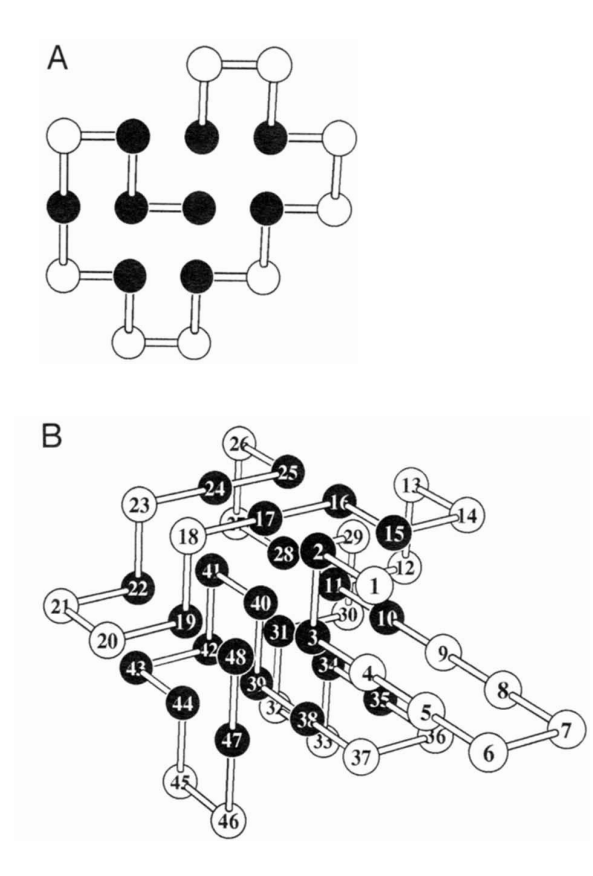
\includegraphics[width=0.5\linewidth]{figures/bioinformatics/hp_model.png}
    \caption{HP model of protein folding\cite{dill_principles_2008}}
\end{figure}

From a single vertex in a 3D grid, we can step in $4$ or $6$ directions: up, down, left, right and inwards and outwards in the 3D case. We can encode these naturally, using one-hot encoding, by introducing $6$ bits of information. If we assume that the chain starts in the origin, then we can encode a chain shape by giving the directions of the $(n-1)$ steps it takes.

A chain like this is viable, when it doesn't cross over itself. A chain's optimality is assessed by counting how many pairs of various aminoacids are neighbouring each other. To answer both of these questions, we must be able to calculate relative distances between any two points of the chain. Using the directinal one-hot encoding model, these questions can be answered by taking the sum of some qubits.

Using these operations, we can create a quantum oracle, that assesses the optimality of a particular chain and use Grover's quantum search algorithm to find the best possible solution.

Unfortunately, while Qiskit itself is open-source, it's architecture (similarly to other quantum computing frameworks) is designed from the core to store the matrices of various operations (such as the WeightedAdder operation) in its memory and retrieve this information during simulation. This means that I am unable to correct this single operation in Qiskit.

\section{Contents of this dissertation}

In order to reduce the memory requirements for any quantum computation simulation, I have to be able to reduce storing large operation matrices in memory whenever I can. This requires a completely different architecture.



\section{Contents of this dissertation}

\subsection{TDK 2021/Dipterv}

The rest of this thesis is structured in the following way: In Chapter 2, I introduce Quantum computing, specifically Quantum Random Walks, in a bottom-up approach, starting from the simplest form and then generalizing it. Contrary to many authors, I use linear algebra exclusively to describe each step since implementation on a universal quantum computer requires the definition to come in the form of unitary transformations.

Section 2.2.5 discusses two of the generalization techniques found in~\cite{Portugal}. I present my improvement to one of these methods, which I have proven to have the equivalent result but remove an exponential memory requirement from the implementation. The other method in~\cite{Portugal} uses a constraint about the evolution operator, for which I have not found proof in the literature. Here, I present my more generalized version of this constraint and the proof I have given.

In Chapter 3, I introduce three bioinformatics problems: DNA sequencing, Protein folding and Molecular docking. I explain the computational models that emerge from these practical problems and the well-known computational problems they reduce to.

In Chapter 4, I describe my simulator software's architecture and implementation details and present the results obtained from my simulation runs.

\subsection{TDK 2022}

The remaining chapters are structured as follows: In Chapter 2 I introduce Grover's search algorithm framework and solve a generalized version of the Sudoku puzzle with it. I iterate over the necessary components from this solution, the particular operators needed for the oracle and the amplitude amplification technique's implementation. In Chapter 3 I lay down the mathematical foundations for a quantum simulator framework's implementation, particularly the solution to applying a quantum operator to a subset of the registers in the system, then I introduce the quantum operators and their implementations in my system. Finally, I describe the architectural design patterns used in the system. In Chapter 4 I summarize the results of this paper and lay down my plans for the future.
\chapter{Bioinformatics}

\section{Computational problems in bioinformatics}

In this chapter, I present an overview of some interesting and important bioinformatical problems, particularly protein folding, which is one of the central problems related to drug discovery\cite{BockenhauerAlgoBioinfo}.

\subsection{DNA sequencing and the Human Genome Project}

The complete genetic material of a human being is called the human genome, which is contained in the nucleus of every single cell of the human body and is replicated during cell division. The human genome consists of 46 chromosomes, each containing a single deoxyribonucleic acid, or DNA molecule for short. A DNA molecule is two twisting, paired strands (called the double helix structure) and comprises around 3.2 billion pairs of nucleotide bases. Nucleotides are usually denoted by the letters A, T, C and G, with A-T and C-G forming pairs. A sequence of nucleotides that together encode the synthesis of a specific protein or RNA is called a gene.

Research into the human genome started with the discovery of the double helix structure of the DNA molecule in 1953 by Francis Crick and James Watson. The Human Genome Project\cite{CollinsHumanGenome1995} was launched in 1990, an international research effort to identify the function of all 50,000 to 100,000 genes of the complete human genetic material and was completed in early 2022\cite{zahn_filling_2022}. Besides injuries, nearly all human medical conditions are related to mutations at specific locations in the structure and function of the genetic material\cite{CollinsHumanGenome1995}, so identifying changes in an individual's DNA sequence can be an indispensable tool for predicting and preventing disease while providing individualized care. This requires a quick sequencing of specific parts of a person's DNA and comparing them to a healthy variant.

\begin{figure}[H]
    \centering
    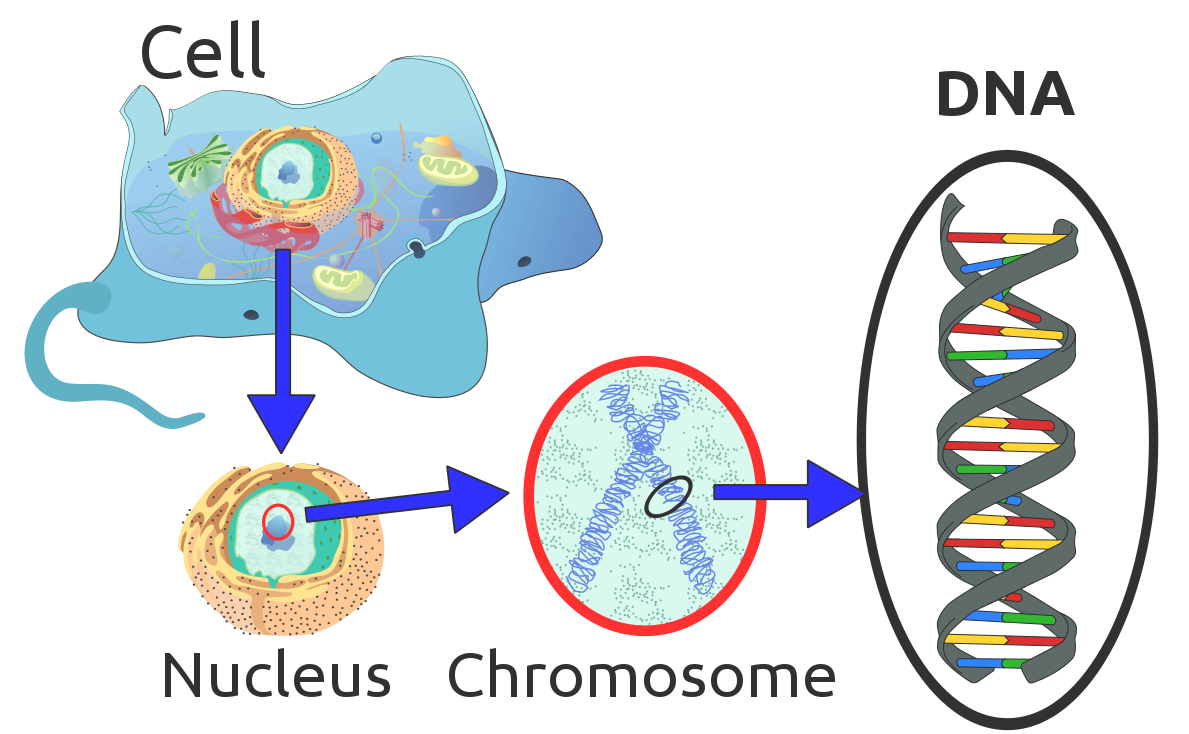
\includegraphics[width=0.6\textwidth]{figures/bioinformatics/dna.png}
    \caption{DNA structure\cite{dna_sequencing}}
\end{figure}

From a computer science viewpoint, a simplified DNA model is a string consisting of the four letters from one of the strands of the physical molecule. (However, this model omits the 3D spatial structure.) Due to the limits of our technology, current methods enable us to read up to 1000 consecutive letters from a single sample. To sequence a longer string, we can break the molecule into sufficiently smaller fragments and sequence them individually. Unfortunately, in this process, the order in which the fragments originally occurred is lost. One possible approach to deal with this problem is to create copies of the DNA molecule we are interested in and randomly break each of these copies into fragments. With a high probability, the resulting fragments from different copies will overlap with each other. Then, the task becomes reconstructing the original string from these fragments while considering the possible errors in our biological measurements. The possible number of fragment orderings is enormously large, so a brute force algorithm does not suffice for solving this task.\cite{CollinsHumanGenome1995}

Between any two humans, the amount of genetic variation is estimated to be around 0.6\%\cite{the_1000_genomes_project_consortium_global_2015}. This enables us to use the targeted part of the genome sequence preassembled by the Human Genome Project and align our obtained DNA sequence fragments to the best fitting position to obtain the entire string of our DNA. Algorithms such as the Smith-Waterman algorithm and the Needleman-Wunsch algorithm can efficiently perform this sequence alignment task.

\subsection{Protein folding}

Proteins are one of the fundamental building blocks of the human body. They play an essential role in our immune system response, transportation of molecules throughout the body, the catalysation of metabolic reactions and signal transmission. Protein molecules consist of a single, long chain of amino acids. While several amino acid molecules exist in nature, only 20 of those are present in proteins.\cite{BockenhauerAlgoBioinfo}

The 20 standard amino acids can be seen in Table \ref{aminoacids20}. The most important property of these is their affinity to water: Some amino acids are polar (hydrophilic), commonly denoted by a P, which means they can establish hydrogen bonds with $H_2O$ molecules. In contrast, others are hydrophobic (nonpolar), commonly denoted by an H, which do not establish these bonds with water.

\begin{table}[H]
\centering
\begin{tabular}{|l|ccc|}
\hline
Name          & Abbreviation & Code & Polarity \\
\hline
Alanine       & Ala & A & H \\
Valine        & Val & V & H \\
Leucine       & Leu & L & H \\
Isoleucine    & Ile & I & H \\
Phenylalanine & Phe & F & H \\
Proline       & Pro & P & H \\
Methionine    & Met & M & H \\
Tryptophan    & Trp & W & H \\
\hline
Arginine      & Arg & R & P \\
Asparagine    & Asn & N & P \\
Aspartic acid & Asp & D & P \\
Cysteine      & Cys & C & P \\
Glutamic acid & Glu & E & P \\
Glutamine     & Gln & Q & P \\
Glycine       & Gly & G & P \\
Histidine     & His & H & P \\
Lysine        & Lys & K & P \\
Serine        & Ser & S & P \\
Threonine     & Thr & T & P \\
Tyrosine      & Tyr & Y & P \\
\hline
\end{tabular}
\caption{Aminoacids in proteins}
\label{aminoacids20}
\end{table}

The functionality and role of a protein are determined by its spatial structure, of which four levels are distinguished.

\textbf{Primary structure}: The sequence of amino acids in the protein.

\begin{figure}[H]
    \centering
    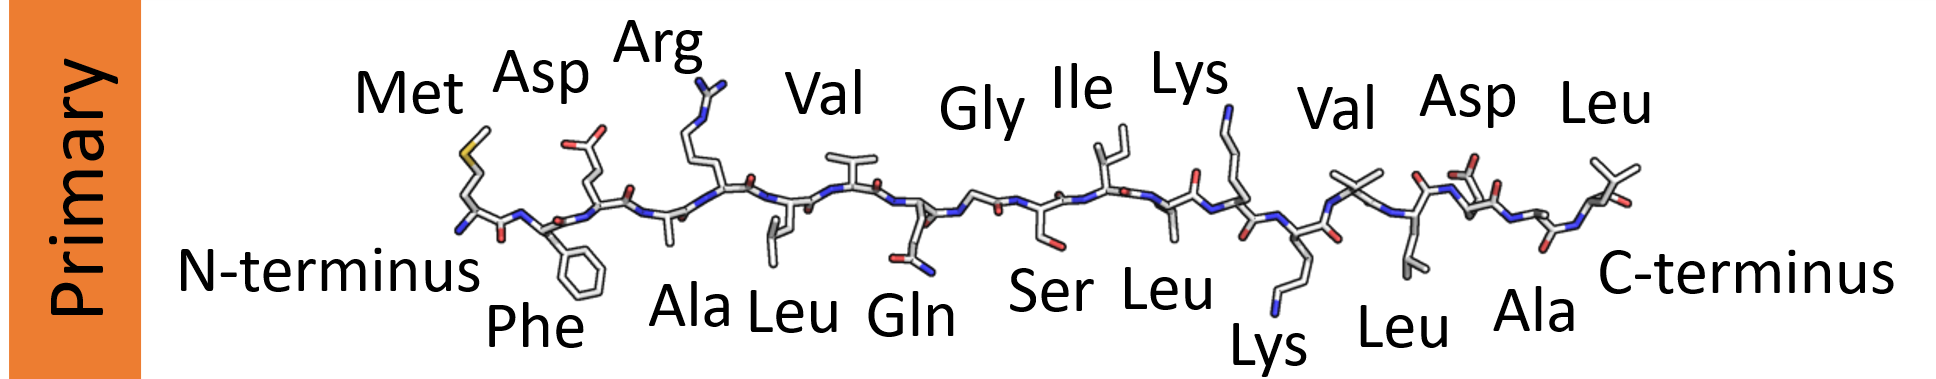
\includegraphics[width=\textwidth]{figures/bioinformatics/protein_structure_primary.png}
    \caption{Primary structure of the protein PCNA\cite{protein_structure}}
\end{figure}

\textbf{Secondary structure}: Created by the interactions between the atoms along the chain of amino acids, forming substructures ($\alpha$-helices, $\beta$-sheets, loops).

\begin{figure}[H]
    \centering
    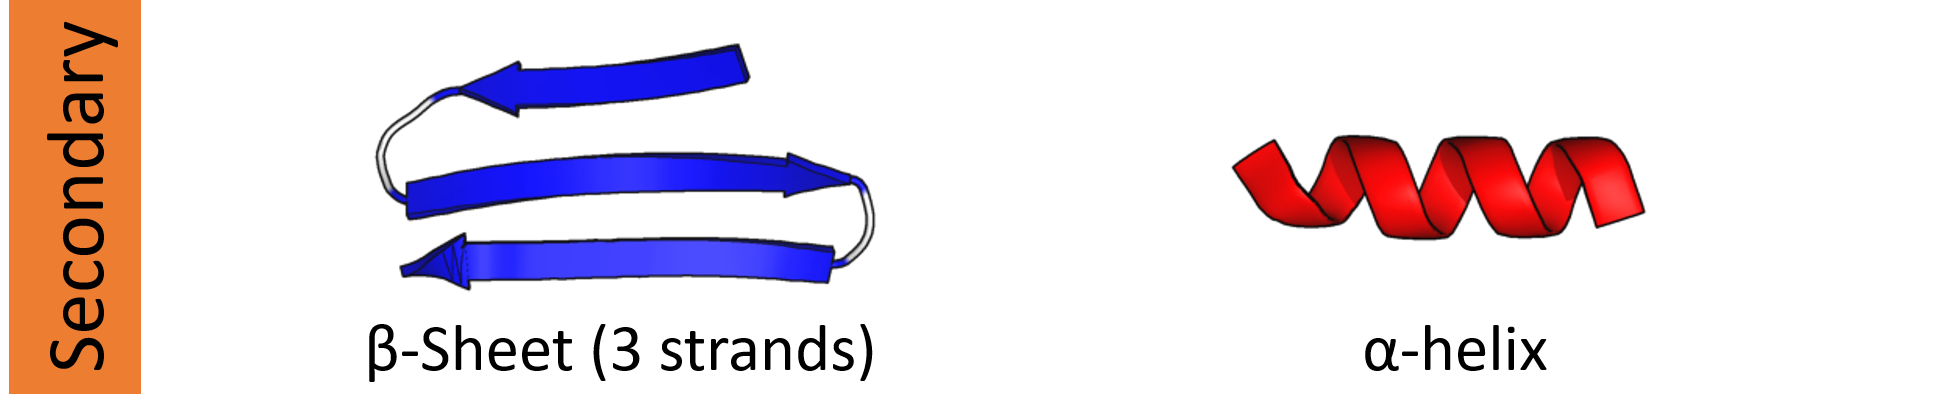
\includegraphics[width=\textwidth]{figures/bioinformatics/protein_structure_secondary.png}
    \caption{Secondary structure of the protein PCNA\cite{protein_structure}}
\end{figure}

\textbf{Tertiary structure}: The spatial arrangement of all atoms within the chain. Secondary structure elements are grouped together as motifs, and functional units called domains.

\begin{figure}[H]
    \centering
    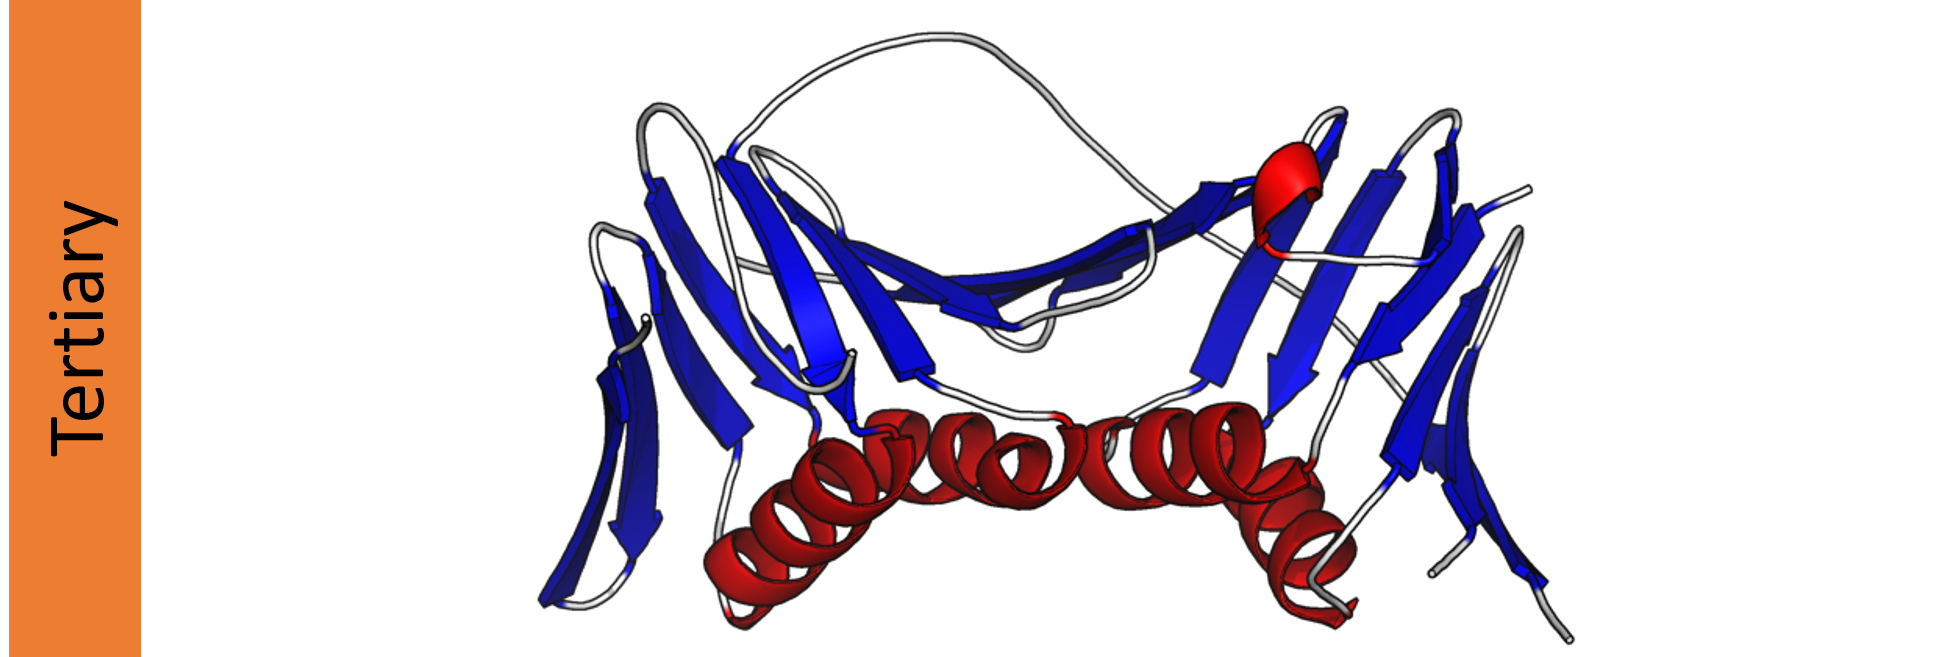
\includegraphics[width=\textwidth]{figures/bioinformatics/protein_structure_tertiary.png}
    \caption{Tertiary structure of the protein PCNA\cite{protein_structure}}
\end{figure}

\textbf{Quaternary structure}: Describes the composition of the whole protein from polypeptide subunits and potentially other molecular parts.

\begin{figure}[H]
    \centering
    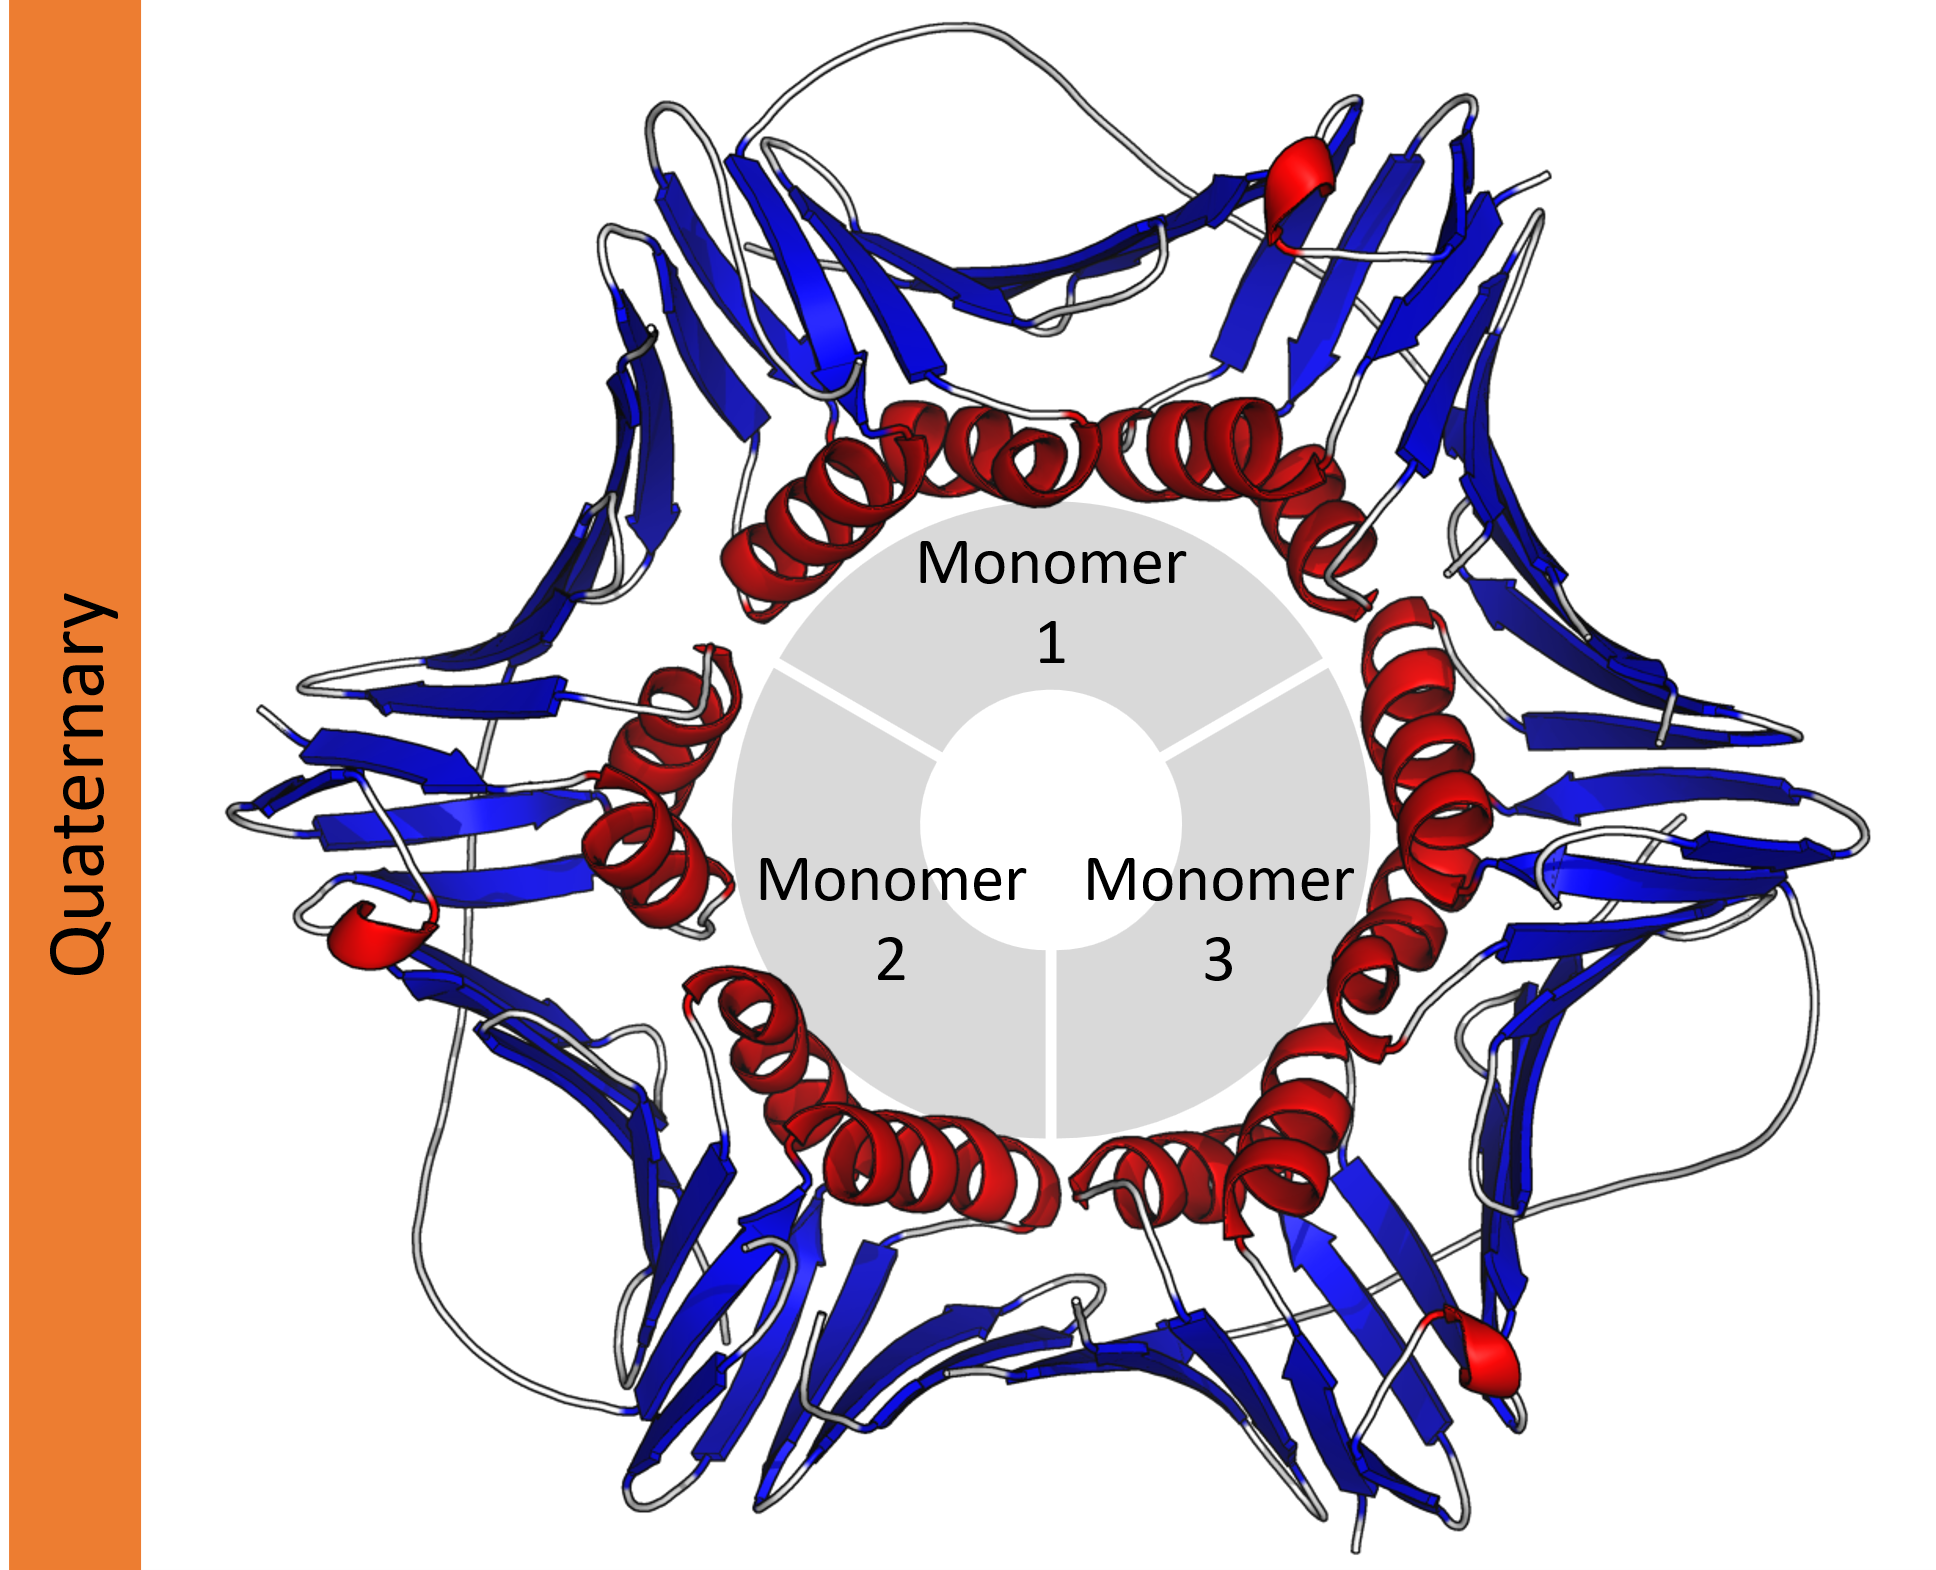
\includegraphics[width=\textwidth]{figures/bioinformatics/protein_structure_quaternary.png}
    \caption{Quaternary structure of the protein PCNA\cite{protein_structure}}
\end{figure}

For example, hemoglobin is a protein found in red blood cells whose function is to carry oxygen molecules throughout the blood vessels. The oxygen molecule binds to the heme groups found in the protein.

\begin{figure}[H]
    \centering
    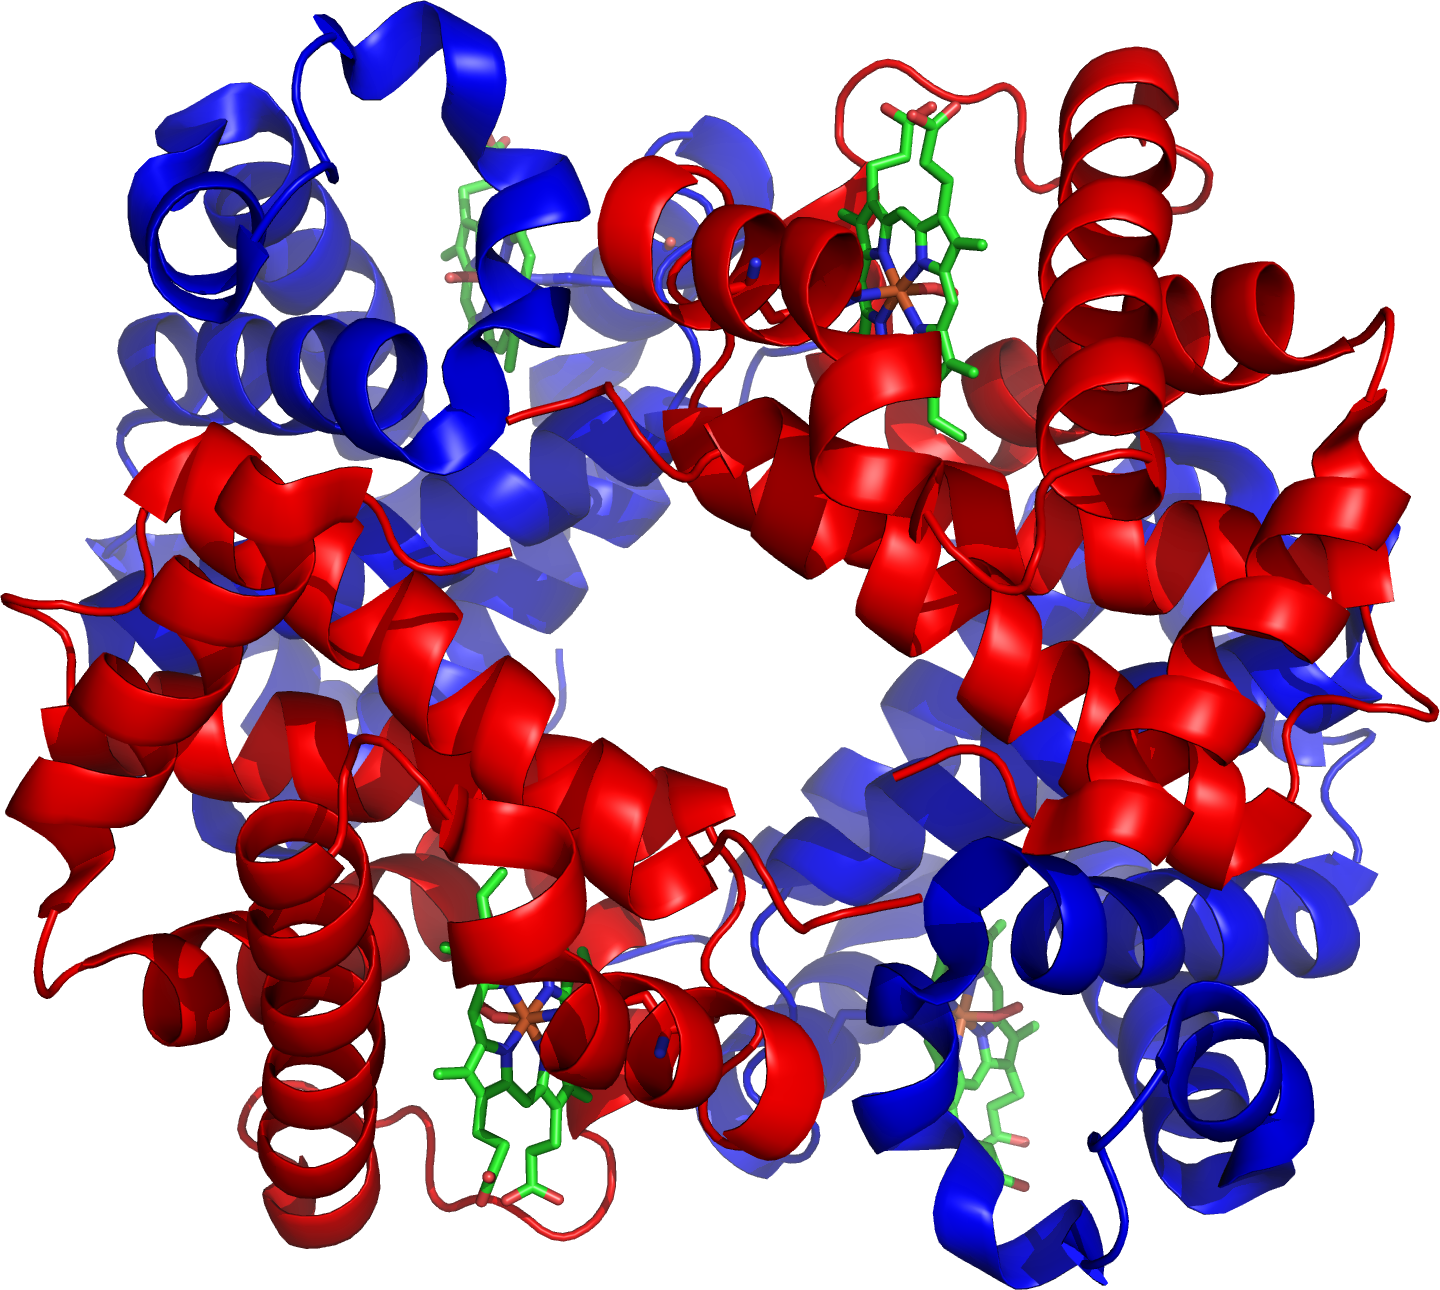
\includegraphics[width=0.5\textwidth]{figures/bioinformatics/hemoglobin.png}
    \caption{Hemoglobin, the iron-containing heme groups are shown in green\cite{wheeler_1gzx_nodate}}
\end{figure}

To understand the function of a protein, we must determine its complete 3D structure. While techniques exist to measure a molecule's structure in real life, these are incredibly time-consuming and expensive to perform, even for a single molecule. Consequently, we would like to design algorithms that can predict the complete 3D structure of a protein based on its primary structure or its amino acid sequence. These algorithms are called protein folding algorithms.

In the molecular docking task, the candidate protein has already been selected with its 3D structure known. For the purpose of drug discovery, we are searching for the best possible protein as well, which is why databases of proteins with their predicted 3D structures are being worked on, such as \href{https://www.uniprot.org/}{https://www.uniprot.org/}, or \href{https://alphafold.ebi.ac.uk/}{https://alphafold.ebi.ac.uk/} \cite{senior_improved_2020}.

Modelling and predicting the complete four levels of protein structure is a complex task. Interestingly, simplified models exist that can be experimentally shown to achieve a reasonable approximation. One of these models was given by Dill et al. in 1995. (republished in 2008) \cite{dill_principles_2008}. Even though these models vastly simplify the real-life behaviour of protein chains, the corresponding algorithmic problem is still NP-hard. Later in my dissertation, I will further discuss Dill's HP model for protein folding.

\subsection{Molecular docking}

Proteins are the primary agents of biological function, as they control the various chemical mechanisms that occur inside the cells. Proteins that act as biological catalysts are called enzymes. Catalysts facilitate various chemical reactions without being consumed in the process. These molecules have a binding site (a 'hole' on their 3D surface), into which only a specific other molecule fits, which is called a substrate. During the chemical reaction, the substrate is turned into other products.  \cite{fionda_networks_2019}

Many human diseases result from abnormal interactions between proteins. In order to prevent disease, we can stop (inhibit) these interactions from happening. This is done by blocking the binding site of the faulty enzyme with another molecule. Conventional medicine uses giant molecules (antibodies) or tiny molecules (like aspirin) to achieve this. The next generation of protein therapeutics currently under development aims to find inhibitors within the family of smaller-sized proteins.
 \cite{ryan_proteinprotein_2005}

In order to inhibit an enzyme's reaction from happening, we must find a protein that folds into a shape that fits into the enzyme's binding site to prevent it from catalyzing a reaction. The analogy of 'lock-and-key' was coined for this by Emil Fischer in 1894. He suggested that the 'lock' describes the enzyme's binding site, and the 'key' describes the missing molecule inhibitor, which has to fit into the 'lock'. \cite{a_molecular_2018} \cite{walker_molecular_2008} The computational task of predicting whether a protein with a known 3D structure will fit inside the binding site of a specific enzyme is called molecular docking.

\begin{figure}[H]
    \centering
    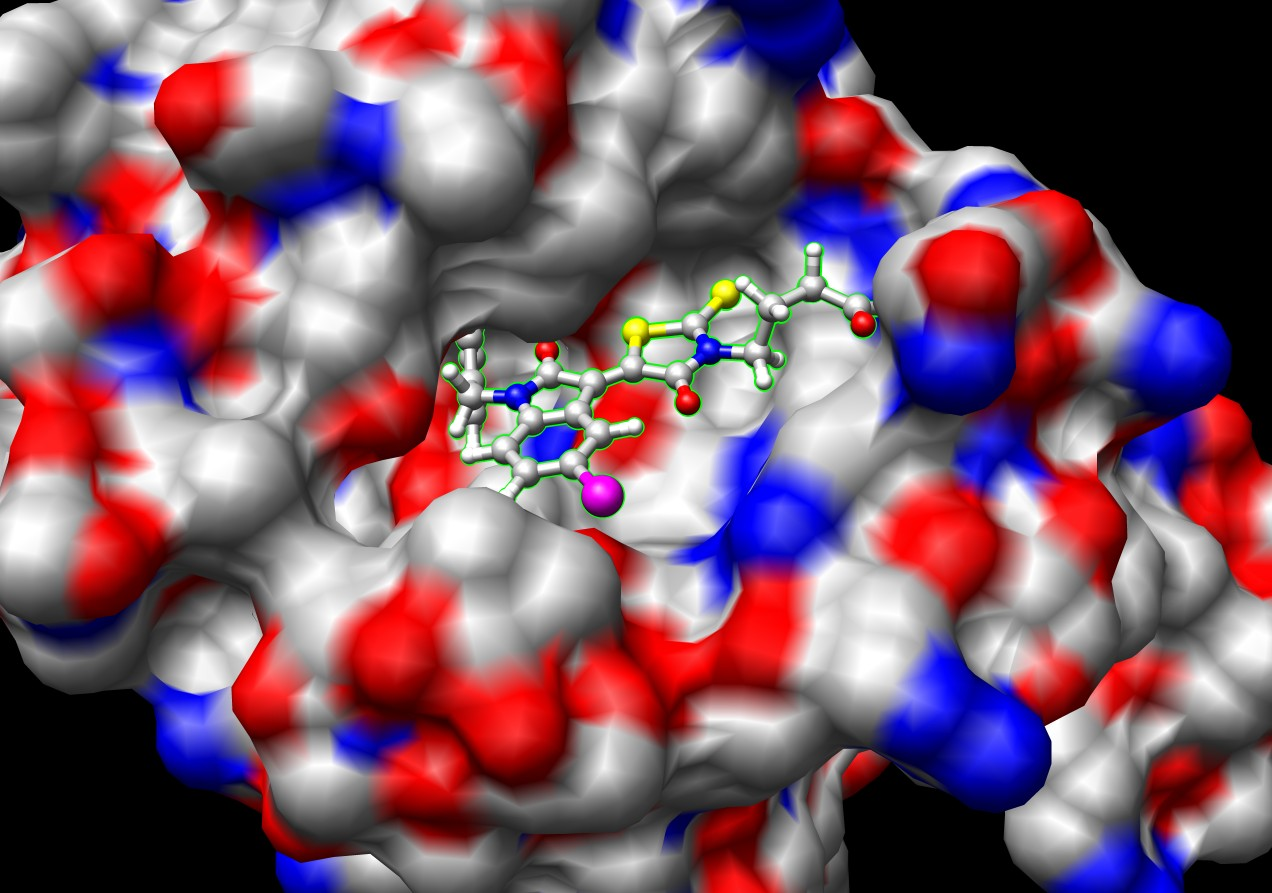
\includegraphics[width=0.8\textwidth]{figures/bioinformatics/molecular_docking.jpg}
    \caption{Molecular docking\cite{chaos_chemical_2008}}
\end{figure}

In the molecular docking problem, both the binding site's 3D structure and the protein's 3D structure are represented by a graph. The graph's vertices are the atoms on the surface. The edges represent a chemical bond between the corresponding atoms. The weight of a given edge represents the physical distance between the atoms. Omitting the edge weights, the problem is analogous to subgraph isomorphy (an NP-hard problem), the binding site's graph representation being a subgraph of the inhibitor molecule's entire surface in a graph representation. With the edge weights present, we can employ a measure that assigns a score to an isomorphy mapping of the vertices between the two graphs. Typically root mean square deviation (RMSD) is used, which can be defined for two sets of (ordered) points. The mapping achieving the highest score is the best theoretical fit for the molecule.
 \cite{wang_protein_2021}

\section{The connection between bioinformatics and quantum algorithms}

While some problems in bioinformatics, such as DNA sequence alignment, already have a fast enough solution, others, such as protein folding and molecular docking, turn out to be NP-hard ones. I have chosen to explore protein folding in more detail.

Grover's search algorithm is a quantum algorithm that can solve problems classically in NP if a candidate solution can be encoded to a quantum register and the verifier algorithm can be translated to quantum gate logic. Applying multiple Grover searches, we can also give a solution that minimizes or maximizes a target function. In the case of protein folding, a candidate solution is a possible orientation of a chain in 3D space, and we are looking for the minimum energy configuration.

Quantum walks work by exploring the problem's domain, which can be represented in a graph form. The vertices are candidate solutions, and the edges connecting them are small transformations on them. In the case of protein folding, a possible small transformation is rotating the chain at a single point. This operation also has to be translated to quantum gate logic.

These two algorithms can be effectively combined. For example, the initialization step for Grover can be a quantum walk, or they can be applied in turns.
\chapter{Quantum computing}

Algorithms in quantum computing are derived from the postulates of quantum mechanics. These fundamental rules define how a quantum computer operates and are essential for any discourse on quantum algorithms.

This introduction is based on the following books: Quantum Computing and Communications by Sándor Imre and Ferenc Balázs~\cite{ImreSandor}, Quantum Computing by Mika Hirvensalo~\cite{Hirvensalo} and Quantum Walks and Search Algorithms by Renato Portugal~\cite{Portugal}.

\lineparagraph{Postulate I. State space}

The state of an isolated physical system can be described using a unit length \textit{state vector} in a Hilbert space (i.e. complex linear vector space), or \textit{state space}, equipped with an inner product.

\begin{definition}[Qubit]
A state vector in the 2 dimensional Hilbert space ($H_2$) is a qubit. The base vectors in this space are

\begin{align*}
\ket{0} = \begin{pmatrix} 1 \\ 0 \end{pmatrix} \text{, and } \ket{1} = \begin{pmatrix} 0 \\ 1 \end{pmatrix}.
\end{align*}

A generic qubit is written in the form

\begin{align*}
a\ket{0} + b\ket{1} = \begin{pmatrix} a \\ b \end{pmatrix}
\end{align*}

where $a, b \in{} \mathds{C}$ and $|a|^2 + |b|^2 = 1$.
\end{definition}

\begin{definition}[Superposition]

A quantum system is said to be in \textit{superpotion}, if its state vector is a linear combination of multiple basis states.

For example $a\ket{0} + b\ket{1}$ is in a superposition of the basis states $\ket{0}$ and $\ket{1}$, with probability amplitudes $a$ and $b$.

\end{definition}

\lineparagraph{Postulate II. Evolution}
\label{PostulateII}

The time evolution of an isolated physical system is described using unitary transformation, which depends only on the starting and finishing time of the evolution.

A \textit{quantum algorithm} is a sequence of unitary operators applied to an initial state.

\begin{definition}[Unitary matrix]
\label{Unitary}

$\mathbf{U}$ is unitary if $\mathbf{U}^{\dagger} = \mathbf{U}^{-1}$  \cite{HalmosLinearAlgebra}.

The following definitions are equivalent:

\begin{enumerate}
    \item $\mathbf{U}$'s rows form an orthonormal basis of $\mathds{C}^n$.
    \item $\mathbf{U}$'s columns form an orthonormal basis of $\mathds{C}^n$.
    \item $\mathbf{U}$ is an isometry: it is injective and preserves length.
    \item $\mathbf{U}$ preserves the inner product.
\end{enumerate}

\end{definition}

\lineparagraph{Postulate III. Measurement}

A quantum measurement is defined by a set of measurement operators $\{\mathbf{M}_m\}$, where $m$ stands for the possible results of the measurement. The probability of measuring $m$ if the system is in state $\ket{v}$ is

\begin{align*}
    P(m | \ket{v}) = \bra{v} \mathbf{M}_m^{\dagger} \mathbf{M}_m \ket{v}.
\end{align*}

The state of the system after measuring $m$ is then

\begin{align*}
    \ket{v'} = \frac{\mathbf{M}_m\ket{v}}{\sqrt{\bra{v} \mathbf{M}_m^{\dagger} \mathbf{M}_m \ket{v}}}.
\end{align*}

The set of measurement operators have to satisfy the following \textit{completeness relation}:

\begin{align*}
    \sum\limits_{m}  \mathbf{M}_m^{\dagger} \mathbf{M}_m = I,
\end{align*}

due to

\begin{align*}
    1 = \sum\limits_{m} P(m | \ket{v}) = \sum\limits_{m} \bra{v} \mathbf{M}_m^{\dagger} \mathbf{M}_m \ket{v}.
\end{align*}

\linesubparagraph{Projective measurement}\label{PostulateIIIProjective}

To distinguish a set of orthonormal states $\{\ket{\varphi_m}\}$, the corresponding measurement operators can be produced as $\mathbf{P}_m = \ket{\varphi_m}\bra{\varphi_m}$, with the following properties.

\begin{property}[$\mathbf{P}_m$ is self adjoint]

\begin{align*}
\mathbf{P}_m^{\dagger} = \mathbf{P}_m
\end{align*}

Since

\begin{align*}
\mathbf{P}_m^{\dagger} =
(\ket{\varphi_m}\bra{\varphi_m})^{\dagger} =
\bra{\varphi_m}^{\dagger}\ket{\varphi_m}^{\dagger} =
\ket{\varphi_m}\bra{\varphi_m} =
\mathbf{P}_m.
\end{align*}

\end{property}

\begin{property}[$\mathbf{P}_m$ is a projection]

\begin{align*}
\mathbf{P}_m\mathbf{P}_m = \mathbf{P}_m
\end{align*}

Since
\begin{align*}
\mathbf{P}_m\mathbf{P}_m =
(\ket{\varphi_m}\bra{\varphi_m})(\ket{\varphi_m}\bra{\varphi_m}) =
\ket{\varphi_m}(\bra{\varphi_m}\ket{\varphi_m})\bra{\varphi_m} =
\ket{\varphi_m}1\bra{\varphi_m} =
\ket{\varphi_m}\bra{\varphi_m} =
\mathbf{P}_m.
\end{align*}

\end{property}

\begin{property}[The $\mathbf{P}_m$ are orthogonal]

\begin{align*}
m \neq n \Rightarrow \mathbf{P}_m\mathbf{P}_n = \mathbf{0}
\end{align*}

Since
\begin{align*}
\mathbf{P}_m\mathbf{P}_n =
(\ket{\varphi_m}\bra{\varphi_m})(\ket{\varphi_n}\bra{\varphi_n}) =
\ket{\varphi_m}(\bra{\varphi_m}\ket{\varphi_n})\bra{\varphi_n} =
\ket{\varphi_m}0\bra{\varphi_n} =
\mathbf{0}.
\end{align*}

\end{property}

From these properties follows, that the probability of measuring $m$ in case of a projective measurement is

\begin{align*}
P(m | \ket{v}) =
\bra{v}\mathbf{P}_m^{\dagger}\mathbf{P}_m \ket{v} =
\bra{v}\mathbf{P}_m\mathbf{P}_m\ket{v} = 
\bra{v}\mathbf{P}_m\ket{v} =
\bra{v}\ket{\varphi_m}\bra{\varphi_m}\ket{v} = |\bra{\varphi_m}\ket{v}|^2.
\end{align*}

For example, the value of a qubit can be any unit length vector in $H_2$, however when we measure it, we will receive one of the base vectors of $H_2$. For $a\ket{0} + b\ket{1}$ we measure $0$ with probability $|a|^2$ and $1$ with probability $|b|^2$.

\lineparagraph{Postulate IV. Composite systems}
\label{PostulateIV}

The state space of an isolated composite physical system is the \textit{tensor product} of the state spaces of the individual components. The current state vector of the composite system is the \textit{tensor product} of the current state vectors of the individual systems.

If $V_1,\dots,V_n$ are the state spaces of the individual systems, then $V_1 \otimes \dots \otimes V_n$ is the composite state space and for $\ket{v_1} \in V_1, \dots, \ket{v_n} \in V_n$ state vectors, $\ket{v_1} \otimes \dots \otimes \ket{v_n} = \ket{v_1,\dots,v_n}$ is the state vector of the composite system.

\begin{definition}[Tensor product]

The tensor product $\mathbf{A} \otimes \mathbf{B}$ of matrix $\mathbf{A}_{(r \times s)}$ and matrix $\mathbf{B}_{(t \times u)}$ is of size $(rt \times su)$ and is defined as follows \cite{HalmosLinearAlgebra}:

\begin{align*}
\text{For }
\mathbf{A} = \begin{pmatrix}
    a_{11} & a_{12} & \dots  & a_{1s} \\
    a_{21} & a_{22} & \dots  & a_{2s} \\
    \vdots & \vdots & \ddots & \vdots \\
    a_{r1} & a_{r2} & \ddots & a_{rs}
\end{pmatrix}
\text{, and }
\mathbf{B} = \begin{pmatrix}
    b_{11} & b_{12} & \dots  & b_{1u} \\
    b_{21} & b_{22} & \dots  & b_{2u} \\
    \vdots & \vdots & \ddots & \vdots \\
    b_{t1} & b_{t2} & \ddots & b_{tu}
\end{pmatrix}
\end{align*}

\begin{align*}
\mathbf{A} \otimes \mathbf{B} = \begin{pmatrix}
    a_{11}\mathbf{B} & a_{12}\mathbf{B} & \dots  & a_{1s}\mathbf{B} \\
    a_{21}\mathbf{B} & a_{22}\mathbf{B} & \dots  & a_{2s}\mathbf{B} \\
    \vdots  & \vdots  & \ddots & \vdots  \\
    a_{r1}\mathbf{B} & a_{r2}\mathbf{B} & \ddots & a_{rs}\mathbf{B}
\end{pmatrix}
\end{align*}

\end{definition}

and has the following properties:

\begin{property}[Associativity]
\begin{align*}
  (\mathbf{A} \otimes \mathbf{B}) \otimes \mathbf{C} = \mathbf{A} \otimes (\mathbf{B} \otimes \mathbf{C})
\end{align*}
\end{property}

\begin{property}[Mixed product property]
\label{TensorMixedProduct}

If the corresponding matrices are compatible, then

\begin{align*}
  (\mathbf{A} \otimes \mathbf{B})(\mathbf{C} \otimes \mathbf{D}) = (\mathbf{A}\mathbf{C}) \otimes (\mathbf{B}\mathbf{D}),
\end{align*}
\end{property}

and as an immediate consequence, we obtain 

\begin{align*}
  (\mathbf{A} \otimes \mathbf{I})(\mathbf{I} \otimes \mathbf{B}) = \mathbf{A} \otimes \mathbf{B}.
\end{align*}

\begin{definition}[Quantum register]

The composite system of $n$ qubits is a \textit{quantum register}, having the composite state space

\begin{align*}
H_2^{\otimes{}n} = H_2 \otimes H_2 \otimes ... \otimes H_2
\end{align*}

and for $\ket{q_{n-1}} \in H_2, \dots, \ket{q_{0}} \in H_2$ individual state vectors, the composite state vector is

\begin{align*}
\ket{q_{n-1}} \otimes \dots \otimes \ket{q_{0}} = \ket{q_{n-1},\dots,q_0}.
\end{align*}

\end{definition}

\begin{definition}[Entangled state]
Any state consisting of multiple qubits, that is not decomposable, i.e. that can not be written in the form of a composite system of qubits is \textit{entangled}.
\end{definition}

For example, the state $\frac{1}{\sqrt{2}}(\ket{00} + \ket{11})$ is entangled, since it can not be written in the form

\begin{align*}
(a_0\ket{0} + a_1\ket{1})\otimes(b_0\ket{0}+b_1\ket{1}) = a_0b_0\ket{00}+a_0b_1\ket{01}+a_1b_0\ket{10}+a_1b_1\ket{11}
\end{align*}

since that would require from $a_0b_0 = a_1b_1 = \frac{1}{\sqrt{2}}$, for all coefficients to be non-zero and from $a_0b_1 = a_1b_0 = 0$ for either $a_0$ or $b_1$ and either $a_1$ or $b_0$ to be zero, which is a contradiction.
\chapter{Quantum walks}

Current technology is yet to produce a significant number of qubits (quantum bits) in a quantum processor, but many believe the amount will increase over the years. The first practical quantum algorithms to be run on these processors are likely to be the ones that use qubits sparingly. Quantum walking, the generalized version of classical random walking, is exactly this kind of algorithm. The number of qubits required to run a quantum walk on a graph is logarithmic in the number of vertices, making it a promising technique for the near future. Furthermore, by extending the quantum walk algorithm with a Grover search, it can be used to perform searching, which could be used for solving many of the computationally hard bioinformatical problems.

\section{Classical random walks}

Before introducing quantum computation and specifically quantum walks, I first overview classical random walks, based on the book Probability and Computing, written by Michael Mitzenmacher and Eli Upfal~\cite{MitzenmacherProbability}.

A \textit{random walk} is a stochastic process modeled by a particular type of Markov chain. While a variety of Markov chains exist, in this work, I use the following definition exclusively.

\begin{definition}[Markov chain]

A discrete time stochastic process $X_0, X_1, X_2, \dots$ on a finite state space $A$ is a Markov chain if it has the Markov property:

\begin{align*}
P(X_k = a_k \mid X_{k-1} = a_{k-1}, \dots, X_0 = a_0) = P(X_k = a_k \mid X_{k-1} = a_{k-1}) \addspace \forall a_0,\dots,a_k\in A.
\end{align*}

\end{definition}

Without loss of generality, we can assume, that $A = \{0,1,\dots,n\}$.

If the Markov chain is homogenous (time-invariant), the probability of moving from state $i \in A$ to state $j \in A$ is independent of $k$, and thus can be shortened the following way:

\begin{align*}
P(X_k = j \mid X_{k-1} = i) = p_{j\leftarrow{}i} = p_{j,i} \addspace \forall k \in \mathds{Z}^+.
\end{align*}

Where $p_{j,i}$ is called the \textit{transition probability} between states $i$ and $j$.

The \textit{transition matrix} $\mathbf{P}$ is formed by the transition probabilities.

\begin{align*}
    \mathbf{P}[j,i] = p_{j,i} 
\end{align*}

It follows, that for each column in $\mathbf{P}$, the sum is $1$.

\begin{align*}
    \sum\limits_{j=0}^{n}\mathbf{P}[j,i] = 1 \addspace \forall i \in \{0,\dots,n\}
\end{align*}

Let the \textit{probability distribution} of the process in the $t$-th step be $\pi_t$. Then, $\pi_t$ can be computed from the starting distribution $\pi_0$ using $\mathbf{P}$.

\begin{align*}
\pi_{t} = \mathbf{P}^t\pi_{0}
\end{align*}

The \textit{stationary distribution} ($\pi$) of the Markov chain is a distribution that does not change with a transition, i.e. $\pi = \mathbf{P}\pi$.

Markov chains can be represented using graphs. A directed, weighted graph $G(V,E)$ with weight function $w:E\rightarrow{}[0,1]$ represents a Markov chain, if $V=A$ and $w(i,j) = \mathbf{P}[j,i]$. If $\mathbf{P}[j,i] = 0$, then $\{i,j\} \not\in E$.

A random walk on graph $G$ starts from $X_0 = a_0$ and visits the vertices of the graph according to the states of the Markov-chain: $X_1 = a_1, X_2 = a_2, \dots$ .

Frequently studied characteristics of random walks are \textit{hitting time}~\cite{XiaReview} and \textit{mixing time}~\cite{MitzenmacherProbability}. Informally, hitting time describes how quickly can a vertex be reached from another vertex in the graph, while mixing time expresses how fast the walk reaches the stationary distribution, where the starting vertex can no longer be identified.

\begin{definition}[Hitting time] Let $h_{j,i}$ be the expected number of steps before node $j$ is visited in a random walk starting from node $i$.
Then, $h_{j,i}$ is given by the following recursive formula:
\begin{align*}
    h_{j,i} = \left\{
        \begin{array}{lr}
            1 + \sum\limits_{k\in{}A}p_{j,k}h_{k,i} & \text{if } i\neq{}j\\
            0 & \text{if } i=j
        \end{array}
    \right.
\end{align*}
\end{definition}

\begin{definition}[Mixing time] The smallest time index of the Markov chain, where the total variational distance between the current and the stationary distribution is not greater than a given $\varepsilon$. This measure still depends on the starting distrubiton $\pi_0$, so we take the maximum over all of the possible $\pi_0$ distributions.

\begin{align*}
m(\varepsilon) = \max\limits_{\pi_0}\{\min\{t : \sum\limits_{j=0}^{n}|\pi_t[j] - \pi[j]| \leq \varepsilon\}\}
\end{align*}

\end{definition}

\section{From classical to quantum}

In classical random walks, the walker moves from the current vertex via one of its outgoing edges, chosen randomly, weighted by the edge weights. This random choice can be interpreted as a (generalized) coin toss.

To formulate a quantum version of graph walking, we define the quantum coin, which will replace the classical concept of randomness with quantum superposition.

\section{Formulating the Quantum coin}

I used Renato Portugal's Quantum Walks and Search Algorithms~\cite{Portugal} book as a reference for the different types of coins presented in this section.

A \textit{quantum coin} is a quantum system, which behaves according to the postulates of quantum mechanics. It has a current state, represented by a state vector in a Hilbert space and a unitary time evolution operator, describing a coin toss.

After tossing the coin, the resulting coin state chooses the next step of the quantum walker. If there are $d$ outgoing edges to choose from, then the coin's state space must have $d$ orthonormal basis states, each corresponding to one of the possible edges. If the current state is one of the basis states, then the walker moves in that direction. However, in the quantum world, the coin can also be in a superposition, consisting of multiple basis states. This means that the walker will simultaneously move in all corresponding directions and occupy more than one vertex at the same time, resulting in the walker spreading over the graph in a superposition.

For the $d$ dimensional coin state, the corresponding coin flip operator is a $(d\times{}d)$ dimensional unitary matrix. Based on what the transition operator is, several types of coins can be defined. The following ones are typically used in quantum walks.

\subsection{Hadamard coin}

The Hadamard coin is the most commonly used quantum coin. It is defined by the Hadamard-matrix as a transition operator:

\begin{align*}
  \mathbf{H} = \frac{1}{\sqrt{2}}\begin{pmatrix}
      1 & 1  \\
      1 & -1
    \end{pmatrix}.
\end{align*}

If the starting coin state is $\ket{0}$, then flipping the coin once results in the following state:

\begin{align*}
 \mathbf{H}\ket{0} = \frac{1}{\sqrt{2}}\begin{pmatrix}
      1 & 1  \\
      1 & -1
    \end{pmatrix} \begin{pmatrix} 1 \\ 0 \end{pmatrix}
    = \frac{1}{\sqrt{2}} \begin{pmatrix} 1 \\ 1 \end{pmatrix} = \frac{1}{\sqrt{2}} \ket{0} + \frac{1}{\sqrt{2}} \ket{1}.
\end{align*}

If we measured the above coin, the probability of measuring $0$ is

\begin{align*}
P(0 \mid \frac{1}{\sqrt{2}} (\ket{0} + \ket{1})) =
\left\lvert\frac{1}{\sqrt{2}}\right\rvert^2 =
\frac{1}{2}.
\end{align*}

Similarly, if the starting coin state is $\ket{1}$, then flipping the coin once results in the following state:

\begin{align*}
   \mathbf{H}\ket{1} = \frac{1}{\sqrt{2}}\begin{pmatrix}
      1 & 1  \\
      1 & -1
    \end{pmatrix} \begin{pmatrix} 0 \\ 1 \end{pmatrix}
    = \frac{1}{\sqrt{2}} \begin{pmatrix} 1 \\ -1 \end{pmatrix} = \frac{1}{\sqrt{2}} \ket{0} - \frac{1}{\sqrt{2}} \ket{1}.
\end{align*}

The probability of measuring $1$ here is similarly

\begin{align*}
P(1 \mid \frac{1}{\sqrt{2}} (\ket{0} - \ket{1})) =
\left\lvert-\frac{1}{\sqrt{2}}\right\rvert^2 =
\frac{1}{2}.
\end{align*}

An unexpected feature of this coin comes from the fact, that the Hadamard-matrix is Hermitian (self-adjoint), i.e. $\mathbf{H}^{\dagger} = \mathbf{H}$, while also unitary, i.e. $\mathbf{H}^{\dagger} = \mathbf{H}^{-1}$, which results in $\mathbf{H}^{-1} = \mathbf{H}$, thus $\mathbf{H}\mathbf{H} = \mathbf{I}$. This means, that after flipping the coin twice without measuring it, it will return the coin state to its origin. For example, starting from $\ket{0}$:

\begin{align*}
 \mathbf{H}^2 \ket{0} = \mathbf{H}\frac{1}{\sqrt{2}}(\ket{0} + \ket{1}) = \frac{1}{2}(\ket{0} + \ket{1} + \ket{0} - \ket{1}) = \ket{0}.
\end{align*}

After the second flip, the probability of measuring $\ket{0}$ is $1$, due to the destructive interference between the two $\ket{1}$ probability amplitudes, demonstrating a significant contrast between classical and quantum walks.

\begin{definition}[$2^n$ dimensional Hadamard-coin]

A $2^n$ dimensional Hadamard-coin operator can be created by taking the tensor product of the $2$ dimensional Hadamard-coin $n$ times: $\mathbf{H}^{\otimes{}n}$.

\end{definition}

\subsection{Grover coin}

The Grover coin originates from Grover's search algorithm, where it is applied as the diffusion operator.

Let $\ket{D}$ be the following state:

\begin{align*}
\ket{D} = \mathbf{H}^{\otimes{}n}\ket{0} =
\frac{1}{\sqrt{2^n}} \sum\limits_{i=0}^{2^n-1} \ket{i}.
\end{align*}

Using $\ket{D}$, the Grover coin is the following unitary matrix:

\begin{align*}
    \mathbf{G} = 2\ket{D}\bra{D} - \mathbf{I}.
\end{align*}

If $N = 2^n$, then $\mathbf{G}$ unrolls to the following representation:

\begin{align*}
  \mathbf{G} = \begin{pmatrix}
      \frac{2}{N} - 1 & \frac{2}{N} & \dots  & \frac{2}{N} \\
      \frac{2}{N} & \frac{2}{N} - 1 & \dots  & \frac{2}{N} \\
      \vdots & \vdots & \ddots & \vdots \\
      \frac{2}{N} & \frac{2}{N} & \ddots & \frac{2}{N} - 1
    \end{pmatrix}.
\end{align*}

\subsection{Fourier coin}

In contrast to the Hadamard and Grover coins, the Fourier coin can be of any size, not just a power of 2. A size $N$ Fourier-coin, $F_N$ is defined by the matrix of the Quantum Fourier Transform:

\begin{align*}
\mathbf{F}[k,l] = \frac{1}{\sqrt{N}} \omega^{kl}
\end{align*}

where $\omega$ is the $N$-th root of unity,

\begin{align*}
\omega = e^{\frac{2\pi{}i}{N}}.
\end{align*}

$\mathbf{F}$ unrolls to the following representation:

\begin{align*}
\mathbf{F} = \frac{1}{\sqrt{N}}
\begin{pmatrix}
  1 & 1 & 1 & \dots & 1 \\
  1 & \omega & \omega^2 & \dots & \omega^{N-1} \\
  1 & \omega^2 & \omega^4 & \dots & \omega^{2(N-1)} \\
  \vdots & \vdots & \vdots & \ddots & \vdots \\
  1 & \omega^{N-1} & \omega^{2(N-1)} & \dots & \omega^{(N-1)(N-1)}
\end{pmatrix}
\end{align*}

\section{Quantum walks on the line}

Kempe introduces quantum walks from a physicist's perspective in~\cite{KempeIntroduction} using a particle characterised by its position on the line $\ket{x}$ and its spin state $\ket{s}$.

\subsection{State space}

\lineparagraph{Spin state}

The spin state is in $H_2$ with the basis states spin up and down:

\begin{align*}
\ket{\uparrow} = \ket{0}, \\
\ket{\downarrow} = \ket{1}.
\end{align*}

The spin state vector is then given by:

\begin{align*}
\ket{s} = s_0 \ket{\uparrow} + s_1 \ket{\downarrow}.
\end{align*}

\lineparagraph{Position state}

At the start of the walk the particle is at the origin $\ket{0}$ and the walking lasts for $N$ steps. The position state is in $H_{(2N+1)}$ with the following basis vectors corresponding to the possible positions on the line.

\begin{align*}
\{
\ket{-N},\ket{-(N-1)},\dots,
\ket{-1},\ket{0},\ket{1},\dots,
\ket{N-1},\ket{N}
\}
\end{align*}

I index the basis states using negative numbers to match the labels on the axis.

The position state vector is then given by:

\begin{align*}
    \ket{x} = \sum\limits_{i=-N}^{N}x_i\ket{i}.
\end{align*}

\lineparagraph{Composite state}

The composite state of the system, according to \hyperref[PostulateIV]{[PostulateIV]} is then

\begin{align*}
    \ket{x}\otimes{}\ket{s}.
\end{align*}

\subsection{Evolution}

The particle travels on the line based on its current spin state:
\begin{itemize}
\item If the current spin state is $\ket{0}$, the particle moves to the left, i.e. from position $\ket{i}$ the particle travels to position $\ket{i-1}$.
\item If the current spin state is $\ket{1}$, the particle moves to the right, i.e. from position $\ket{i}$ the particle travels to position $\ket{i+1}$.
\end{itemize}

This step is realised with the unitary matrix $\mathbf{S}$ which operates on the complete state of the system, $\ket{x}\otimes{}\ket{s}$ and is assembled from a left and a right shift operator acting on $\ket{x}$ and another operator for checking $\ket{s}$ compiled using tensor product.

\begin{definition}[Left shift operator]

To move from position $\ket{i}$ to the left ($\ket{i-1}$) the position vector is multiplied with the following $\mathbf{L}$ matrix, containing $1$'s above the diagonal. To keep $\mathbf{S}$ unitary, an unused transition must be added in the lower left corner (see \hyperref[PermutationMatricesTheorem]{Theorem \ref{PermutationMatricesTheorem})}.

\begin{align}
\label{LeftShift}
\mathbf{L} = \ket{N}\bra{-N} + \sum\limits_{i=-(N-1)}^{N} \ket{i-1}\bra{i} =
\left(
    \begin{array}{ccccc}
        0      & 1      & 0      & \cdots & 0      \\
               & \ddots & \ddots & \ddots & \vdots \\
        \vdots &        & \ddots & \ddots & 0      \\
        0      &        &        & \ddots & 1      \\
        1      & 0      & \cdots &        & 0
      \end{array}
\right)
\end{align}

For a given basis vector $\ket{j}$ only one of the summands in $\mathbf{L}$ is non-zero, where $i=j$, resulting in the required shift being performed.

\begin{align*}
\mathbf{L}\ket{j} = \ket{j-1}\bra{j}\ket{j} = \ket{j-1}
\end{align*}

\end{definition}

\begin{definition}[Right shift operator]

To move from position $\ket{i}$ to the right ($\ket{i+1}$) the position vector is multiplied with the following $\mathbf{R}$ matrix, containing $1$'s under the diagonal. To keep $\mathbf{S}$ unitary, an unused transition must be added in the top right corner (see \hyperref[PermutationMatricesTheorem]{Theorem \ref{PermutationMatricesTheorem})}.

\begin{align}
\label{RightShift}
\mathbf{R} = \ket{-N}\bra{N} + \sum\limits_{i=-N}^{N-1} \ket{i+1}\bra{i} =
\left(
    \begin{array}{ccccc}
        0      &        & \cdots & 0      & 1      \\
        1      & \ddots &        &        & 0      \\
        0      & \ddots & \ddots &        & \vdots \\
        \vdots & \ddots & \ddots & \ddots &        \\
        0      & \cdots & 0      & 1      & 0
      \end{array}
\right)
\end{align}

For a given basis vector $\ket{j}$ only one of the summands in $\mathbf{R}$ is non-zero, where $i=j$, resulting in the required shift being performed.

\begin{align*}
\mathbf{R}\ket{j} = \ket{j+1}\bra{j}\ket{j} = \ket{j+1}
\end{align*}

\end{definition}

\lineparagraph{Shift operator}

Using matrixes $L$ and $R$ operating on the position register $\ket{x}$ only, we construct a unitary operator $S$, which operates on the composite state of the system, $\ket{x} \otimes \ket{s}$, executing matrix $\mathbf{L}$ on $\ket{x}$ only when $\ket{s} = \ket{0}$ and matrix $\mathbf{R}$ only when $\ket{s}=\ket{1}$.

\begin{align}
\label{ShiftOperator}
  \mathbf{S} = \mathbf{L}\otimes\ket{0}\bra{0} + \mathbf{R}\otimes\ket{1}\bra{1}
\end{align}

The execution logic is as follows:

\begin{gather*}
    \mathbf{S}(\ket{x}\otimes{}\ket{s}) = \\
    (\mathbf{L}\otimes\ket{0}\bra{0} + \mathbf{R}\otimes\ket{1}\bra{1})(\ket{x}\otimes{}\ket{s}) = \\ (\mathbf{L}\otimes\ket{0}\bra{0})(\ket{x}\otimes{}\ket{s}) + (\mathbf{R}\otimes\ket{1}\bra{1})(\ket{x}\otimes{}\ket{s}) = \dots
\end{gather*}

using \hyperref[TensorMixedProduct]{[TensorMixedProduct]}:

\begin{gather*}
    \dots = \mathbf{L}\ket{x}\otimes(\ket{0}\bra{0}\ket{s}) + \mathbf{R}\ket{x}\otimes(\ket{1}\bra{1}\ket{s}) = \\
    \ket{x-1}\otimes{}s_0\ket{0} + \ket{x+1}\otimes{}s_1\ket{1} = \\
    s_0\ket{x-1, 0} + s_1\ket{x+1,1}.
\end{gather*}

\begin{itemize}
\item If the spin state was $\ket{s} = \ket{0}$ at the beginning, then $s_0=1$ and $s_1=0$, which means that the resulting system state is $\ket{x-1,0}$, which means that the particle shifted to the left, as designed.
\item If the spin state was $\ket{s} = \ket{1}$ at the beginning, then $s_0=0$ and $s_1=1$, which means that the resulting system state is $\ket{x+1,1}$, which means that the particle shifted to the right, also as intended.
\end{itemize}

Furthermore, the spin state can be any mixed state $s_0\ket{0} + s_1\ket{1}$ as well. In this case the particle will shift \textit{both} to the left and to the right, at the same time. When measured, the particle can be found in position $\ket{x-1}$ with probability $|s_0|^2$ and in position $\ket{x+1}$ with probability $|s_1|^2$.

In quantum graph walks, the walker can simultaneously explore multiple parallel paths in the graph, at the same time. With good design, this behaviour can be used to search the graph faster than in classical random graph walks.

\lineparagraph{Coin operator}

To inject the quantum superposition into the walk, the particle's spin state is transformed using any $2$ dimensional unitary matrix between shift operations. The Hadamard, Grover and Fourier coins mentioned earlier are commonly used as coin operators.

For any $C$ operator on the coin register, the unitary transform for the composite system is defined as follows:

\begin{align*}
    \mathbf{\hat{C}} = \mathbf{I} \otimes \mathbf{C}
\end{align*}

since the coin operator does not modify the position register.

\lineparagraph{Evolution operator}

Combining the shift operator and the coin operator together, we obtain the following evolution operator, defining one step of the quantum walk on the line. The step consists of flipping the coin once, then applying the shifting the walker's position accordingly, as follows:

\begin{align*}
    \mathbf{U} = \mathbf{S}\mathbf{\hat{C}} = \mathbf{S}(\mathbf{I}\otimes{}\mathbf{C})
\end{align*}

\subsection{Measurement}

To measure the probability of the particle being at position $\ket{i}$, the projective measurement operator acting on $\ket{x}$ is defined as $\mathbf{P_i} = \ket{i}\bra{i}$, in accordance with \hyperref[PostulateIIIProjective]{[PostulateIIIProjective]}.

Since the coin register need not be measured, we apply the identity operator on it, using $\mathbf{P_i} \otimes \mathbf{I}$ on the complete system to measure the particle's current position.

The probability of finding the particle in position $i$ is:

\begin{gather*}
    P(i | \ket{x}) = \bra{x,s}\mathbf{P_i}\otimes{}\mathbf{I}\ket{x,s} = \dots
\end{gather*}

using \hyperref[TensorMixedProduct]{[TensorMixedProduct]}:

\begin{gather*}
    \dots = \bra{x}\mathbf{P_i}\ket{x}\bra{s}\mathbf{I}\ket{s} =
    \bra{x}\mathbf{P_i}\ket{x}1 =
    \bra{x}\mathbf{P_i}\ket{x} =
    \bra{x}\ket{i}\bra{i}\ket{x} =
    |\bra{i}\ket{x}|^2 =
    |x_i|^2
\end{gather*}

\section{Generalization of Quantum Walks}

After presenting quantum walking on the line, I review and extend two approaches to generalize it in this chapter.

\begin{enumerate}
    \item \textbf{Section \ref{quantum-walk-multiple-2D-coins}: Use multiple two-dimensional coins}: In~\cite{Portugal}, Renato Portugal shows the generalization of quantum walks on a line to a two-dimensional grid, using a method with 2 two-dimensional coins. In this work, I prove how his method reduces to effectively two synchronous independent walks on the $x$ and $y$ axes. Then I improve his technique by generalizing to arbitrarily large dimensional grids in a more memory-efficient way than what would naturally follow from his description.
    \item \textbf{Section \ref{quantum-walk-one-highD-coin}: Use a single higher dimensional coin}: In~\cite{Portugal}, Renato Portugal describes the generalization of a quantum walk on a line to an arbitrary undirected graph and gives the necessary condition for creating the unitary transition matrix without proof. In this work, I generalize to directed graphs and give proof of the generalization of the condition using directed graphs.
\end{enumerate}

\subsection{Generalization using multiple independent 2 dimensional coins}
\label{quantum-walk-multiple-2D-coins}

In \cite{Portugal}, Renato Portugal defines the following method for Quantum Walking on a 2D grid:

Let the position state of the walker be $\ket{x,y}$ and the two coins $\ket{c_x}$, acting on the $x$ coordinate and $\ket{c_y}$, acting on the $y$ coordinate of the walker.

The shift operator moves the walker on the grid diagonally, according to the current state of the two coins, described by

\begin{align}
\label{Portugal2DShift}
    \mathbf{S}\ket{x,y}\ket{c_x}\ket{c_y} = \ket{x + (-1)^{c_x}, y + (-1)^{c_y}}\ket{c_x}\ket{c_y},
\end{align}

and the coin operator leaves the position state in place while flipping both coins at the same time, described by

\begin{align}
\mathbf{\hat{C}} = \mathbf{I} \otimes \mathbf{C_4} = \mathbf{I} \otimes (\mathbf{C_2} \otimes \mathbf{C_2}).
\end{align}

\lineparagraph{Issues with this method}

In \ref{Portugal2DShift}, we can see how the matrix $\mathbf{S}$ will quickly increase in size, as further dimensions are
added to the equation. In 2D, if the walker takes $N$ steps, the size of $\mathbf{S}$ is

\begin{align*}
(2N+1)^2(2N+1)^22^22^2 = 16(2N+1)^4 = O(N^4).
\end{align*}

To increase the dimension count, one would naturally append more coordinates to the composite position state and add further coins, for example in 3D $\mathbf{S}$ would become

\begin{align*}
    \mathbf{S}\ket{x,y,z}\ket{c_x}\ket{c_y}\ket{c_z} =
    \ket{x + (-1)^{c_x}, y + (-1)^{c_y}, z + (-1)^{c_z}}\ket{c_x}\ket{c_y}\ket{c_z},
\end{align*}

For a dimension count $d$, the size of $\mathbf{S}$ is exponential in $d$.

\begin{align*}
((2N+1)^2)^d(2^2)^d = (4(2N+1)^2)^d = O(N^{2d}).
\end{align*}

\lineparagraph{My improvements}

Since in \ref{Portugal2DShift} the coordinates of the walker are updated independently by the separate coins, I was able to disassemble $\mathbf{S}$ into smaller matrices, using the properties of the tensor product.

To do this, in what follows, I first define $\mathbf{S}$ in 2D explicitly (as opposed to the implicit definition in \ref{Portugal2DShift}, stating only how $\mathbf{S}$ updates the state of the system). I will be using the matrices $\mathbf{L}$ defined by Equation (\ref{LeftShift}) and $\mathbf{R}$ defined by Equation (\ref{RightShift}).

Notice that $\mathbf{R}$ increases the walker's coordinates on the line, while $\mathbf{L}$ decreases them. This means, that on the $y$ axis $\mathbf{R}$ acts by moving the walker up, and $\mathbf{L}$ acts by moving the walker down.

When the coins are in the state $\ket{c_x,c_y} = \ket{0,0}$, the walker moves up and to the right. This movement is captured by $\mathbf{S}_{0,0}$, acting on the position state:

\begin{align*}
    \mathbf{S}_{0,0} =  \mathbf{R} \otimes \mathbf{R}
\end{align*}

The other three $\mathbf{S}_{c_x,c_y}$ matrices are defined similarly: 

\begin{align*}
    \mathbf{S}_{0,1} =  \mathbf{R} \otimes \mathbf{L}\\
    \mathbf{S}_{1,0} =  \mathbf{L} \otimes \mathbf{R}\\
    \mathbf{S}_{1,1} =  \mathbf{L} \otimes \mathbf{L}
\end{align*}

Then, I assemble $\mathbf{S}$ using $\mathbf{S}_{0,0}$, $\mathbf{S}_{0,1}$, $\mathbf{S}_{1,0}$ and $\mathbf{S}_{1,1}$ the following way:
\begin{itemize}
\item $\mathbf{S}_{0,0}$ acts only when $\ket{c_x,c_y} = \ket{0,0}$,
\item $\mathbf{S}_{0,1}$ acts only when $\ket{c_x,c_y} = \ket{0,1}$,
\item $\mathbf{S}_{1,0}$ acts only when $\ket{c_x,c_y} = \ket{1,0}$, and finally
\item $\mathbf{S}_{1,1}$ acts only when $\ket{c_x,c_y} = \ket{1,1}$.
\end{itemize}

Using the same method as in Equation (\ref{ShiftOperator}) I arrive at:

\begin{align*}
    \mathbf{S} =
    \mathbf{S}_{0,0} \otimes \ket{0,0}\bra{0,0} + \\
    \mathbf{S}_{0,1} \otimes \ket{0,1}\bra{0,1} + \\
    \mathbf{S}_{1,0} \otimes \ket{1,0}\bra{1,0} + \\
    \mathbf{S}_{1,1} \otimes \ket{1,1}\bra{1,1}\phantom{+}
\end{align*}

After substituting the $\mathbf{S}_{c_x,c_y}$ matrices in:

\begin{align*} 
    \mathbf{S} =   
    (\mathbf{R} \otimes \mathbf{R}) \otimes \ket{0,0}\bra{0,0} + \\
    (\mathbf{R} \otimes \mathbf{L}) \otimes \ket{0,1}\bra{0,1} + \\
    (\mathbf{L} \otimes \mathbf{R}) \otimes \ket{1,0}\bra{1,0} + \\
    (\mathbf{L} \otimes \mathbf{L}) \otimes \ket{1,1}\bra{1,1}\phantom{+}
\end{align*}

Let us name the coin state $\ket{0}$ heads and the coin state $\ket{1}$ tails. Then, using the following equalities and introducing matrices $\mathbf{H}$ and $\mathbf{T}$, as shorthands:

\begin{align*} 
    \ket{0,0}\bra{0,0} = (\ket{0}\bra{0}) \otimes (\ket{0}\bra{0}) = \mathbf{H} \otimes \mathbf{H} \\
    \ket{0,1}\bra{0,1} = (\ket{0}\bra{0}) \otimes (\ket{1}\bra{1}) = \mathbf{H} \otimes \mathbf{T} \\
    \ket{1,0}\bra{1,0} = (\ket{1}\bra{1}) \otimes (\ket{0}\bra{0}) = \mathbf{T} \otimes \mathbf{H} \\
    \ket{1,1}\bra{1,1} = (\ket{1}\bra{1}) \otimes (\ket{1}\bra{1}) = \mathbf{T} \otimes \mathbf{T}
\end{align*}

I arrive at:

\begin{align*} 
    \mathbf{S} =   
    (\mathbf{R} \otimes \mathbf{R}) \otimes (\mathbf{H} \otimes \mathbf{H}) + \\
    (\mathbf{R} \otimes \mathbf{L}) \otimes (\mathbf{H} \otimes \mathbf{T}) + \\
    (\mathbf{L} \otimes \mathbf{R}) \otimes (\mathbf{T} \otimes \mathbf{H}) + \\
    (\mathbf{L} \otimes \mathbf{L}) \otimes (\mathbf{T} \otimes \mathbf{T})\phantom{+}
\end{align*}

Then, using \hyperref[TensorMixedProduct]{[TensorMixedProduct]} I inflate the equation with (appropriately sized) $\mathbf{I}$ matrices:

\begin{align*} 
    \mathbf{S} =   
    ((\mathbf{R} \otimes \mathbf{I})(\mathbf{I} \otimes \mathbf{R})) \otimes ((\mathbf{H} \otimes \mathbf{I}) (\mathbf{I} \otimes \mathbf{H})) + \\
    ((\mathbf{R} \otimes \mathbf{I})(\mathbf{I} \otimes \mathbf{L})) \otimes ((\mathbf{H} \otimes \mathbf{I}) (\mathbf{I} \otimes \mathbf{T})) + \\
    ((\mathbf{L} \otimes \mathbf{I})(\mathbf{I} \otimes \mathbf{R})) \otimes ((\mathbf{T} \otimes \mathbf{I}) (\mathbf{I} \otimes \mathbf{H})) + \\
    ((\mathbf{L} \otimes \mathbf{I})(\mathbf{I} \otimes \mathbf{L})) \otimes ((\mathbf{T} \otimes \mathbf{I}) (\mathbf{I} \otimes \mathbf{T}))\phantom{+}
\end{align*}

At this point, I introduce a few aliases to make the equation more manageable. Notice, how for example $\mathbf{I} \otimes \mathbf{R}$ is acting on the 2D position state, but only updating the $y$ coordinate to move the walker upward. This
gives a way to naturally define $\mathbf{S}_{\text{up}} = \mathbf{I} \otimes \mathbf{R}$, and similarly:

\begin{align*} 
\mathbf{S}_{\text{right}} = \mathbf{R} \otimes \mathbf{I} \\
\mathbf{S}_{\text{left}} = \mathbf{L} \otimes \mathbf{I} \\
\mathbf{S}_{\text{up}} = \mathbf{I} \otimes \mathbf{R} \\
\mathbf{S}_{\text{down}} = \mathbf{I} \otimes \mathbf{L} \\
\end{align*}

At the same time, for example $\mathbf{I} \otimes \mathbf{H}$ is acting on the composite coin state, but only checking if the second coin's state is heads, which is the coin for the $y$ axis. This gives a way to naturally define $\mathbf{H}_y = \mathbf{I} \otimes \mathbf{H}$, and similarly:

\begin{align*} 
\mathbf{H}_x = \mathbf{H} \otimes \mathbf{I} \\
\mathbf{T}_x = \mathbf{T} \otimes \mathbf{I} \\
\mathbf{H}_y = \mathbf{I} \otimes \mathbf{H} \\
\mathbf{T}_y = \mathbf{I} \otimes \mathbf{T} \\
\end{align*}

Substituting all of the aliases:

\begin{align*} 
    \mathbf{S} =   
    (\mathbf{S}_{\text{right}}\mathbf{S}_{\text{up}}) \otimes (\mathbf{H}_x\mathbf{H}_y) + \\
    (\mathbf{S}_{\text{right}}\mathbf{S}_{\text{down}}) \otimes (\mathbf{H}_x\mathbf{T}_y) + \\
    (\mathbf{S}_{\text{left}}\mathbf{S}_{\text{up}}) \otimes (\mathbf{T}_x\mathbf{H}_y) + \\
    (\mathbf{S}_{\text{left}}\mathbf{S}_{\text{down}}) \otimes (\mathbf{T}_x\mathbf{T}_y)\phantom{+}
\end{align*}

Then, using \hyperref[TensorMixedProduct]{[TensorMixedProduct]} again, I arrive at:

\begin{align*} 
    \mathbf{S} =   
    (\mathbf{S}_{\text{right}} \otimes \mathbf{H}_x) (\mathbf{S}_{\text{up}} \otimes \mathbf{H}_y) + \\
    (\mathbf{S}_{\text{right}} \otimes \mathbf{H}_x) (\mathbf{S}_{\text{down}} \otimes \mathbf{T}_y) + \\
    (\mathbf{S}_{\text{left}} \otimes \mathbf{T}_x) (\mathbf{S}_{\text{up}} \otimes \mathbf{H}_y) + \\
    (\mathbf{S}_{\text{left}} \otimes \mathbf{T}_x) (\mathbf{S}_{\text{down}} \otimes \mathbf{T}_y)\phantom{+}
\end{align*}

Then using the distributive property of matrix multiplication with respect to matrix addition I finally arrive at:

\begin{align*} 
    \mathbf{S} =   
    ((\mathbf{S}_{\text{right}} \otimes \mathbf{H}_x) + (\mathbf{S}_{\text{left}} \otimes \mathbf{T}_x))
    ((\mathbf{S}_{\text{up}} \otimes \mathbf{H}_y) + (\mathbf{S}_{\text{down}} \otimes \mathbf{T}_y))
\end{align*}

We can see from the equation above, that $\mathbf{S}$ is actually the product of two shift operators, one only acting on the $x$ coordinate using the first coin's state, the other acting only on the $y$ coordinate, according to the second coin's state.

\begin{align*} 
    \mathbf{S}_x = (\mathbf{S}_{\text{right}} \otimes \mathbf{H}_x) + (\mathbf{S}_{\text{left}} \otimes \mathbf{T}_x) \\
    \mathbf{S}_y = (\mathbf{S}_{\text{up}} \otimes \mathbf{H}_y) + (\mathbf{S}_{\text{down}} \otimes \mathbf{T}_y)
\end{align*}

\vspace{-0.7cm}

\begin{align*}
    \mathbf{S} = \mathbf{S}_x\mathbf{S}_y
\end{align*}

This proves, that the walk on the 2D grid decomposes into two independent line walks on the axes, since $\mathbf{S}_x$ only touches the $x$ coordinate and the first coin, while $\mathbf{S}_y$ only touches the $y$ coordinate and the second coin and there is no entanglement between the registers of the $x$ and $y$ axes. Using this fact, we can simply simulate two independent quantum walks on the line in parallel, or sequentially, using the same registers, which wastly decreases the memory needs of the algorithm. Running in parallel, the memory needs is now $d(4(2N+1)^2) = O(dN^2)$, or running sequentially $(4(2N+1))^2 = O(N^2)$, however the latter uses $dN$ steps, instead of $N$, and $d$ measurements, instead of $1$.

\subsection{Generalization using a single higher dimensional coin}
\label{quantum-walk-one-highD-coin}

Using this method, we generalize quantum walking to arbitrary directed graphs. To do so, we first generalize to regular graphs, then discuss how non-regular graphs can be regularized.

In a $d$-regular graph, the vertices have $d$ neighbours, meaning the walker must choose from $d$ possible directions at every step. Thus the coin is $d$ dimensional. Using this idea as a starting point, we can reverse engineer the generalized walk from the walk on the line by starting from the evolution operator, which assumes nothing about the given graph or coin.

\begin{align*}
    \mathbf{U} = \mathbf{S} \mathbf{\hat{C}} = \mathbf{S} (\mathbf{I} \otimes \mathbf{C})
\end{align*}

In this equation, $\mathbf{C}$ can be any $d$-dimensional unitary matrix. The definition of $\mathbf{S}$ requires more thought, since $\mathbf{S}$ has to encode the graph's structure, while also satisfying \hyperref[PostulateII]{[PostulateII]}.

In one dimension, $\mathbf{S}$ was defined the following way:

\begin{align*}
\mathbf{S} = \mathbf{L}\otimes\ket{0}\bra{0} + \mathbf{R}\otimes\ket{1}\bra{1}.
\end{align*}

$\ket{0}\bra{0}$ and $\ket{1}\bra{1}$ were matrices that checked the current state of the coin and ''activated'' the transition $\mathbf{L}$ or $\mathbf{R}$ accordingly. In $d$ dimensions, the coin has $d$ possible states, i.e. ''sides''

\begin{align*}
    \{\ket{0}, \ket{1}, \dots, \ket{d-1}\},
\end{align*}

which means $\mathbf{S}$ will be constructed using $d$ transition matrices, describing the graph's structure

\begin{align*}
    \mathbf{S} = \mathbf{S}_0\ket{0}\bra{0} + \mathbf{S}_1\ket{1}\bra{1} + \dots + \mathbf{S}_{d-1}\ket{d-1}\bra{d-1}.
\end{align*}

In the 1 dimensional case $\mathbf{L}$ and $\mathbf{R}$ described stepping to the left and to the right, which are
the directed edges of the line graph and $\mathbf{L} + \mathbf{R}$ is the adjacency matrix of the line graph. To generalize this, $\mathbf{S}_0 + \mathbf{S}_1 + \dots + \mathbf{S}_{d-1}$ is going to be the adjacency matrix of the $d$-regular graph.

The question is how do we construct the matrices $\mathbf{S}_0, \mathbf{S}_1, \dots, \mathbf{S}_{d-1}$ from a given adjacency matrix of a $d$-regular graph? It turns out, that in order for $\mathbf{S}$ to satisfy \hyperref[PostulateII]{[PostulateII]}, there are strict rules on how these $\mathbf{S}_i$ matrices can be defined.

It seems to be a well-known fact in the literature, that for $d$-regular undirected graphs with a valid edge coloring using $d$ colors, a possible choice for the sides of the coin correspond to the colorsets of the edges. This means, that the $S_i$ adjacency matrix contains all of the edges that have the $i$th color assigned to them, in both directions (i.e. $S_i$ is symmetric). This is also mentioned in \cite{Portugal}, however no proof is given in this book or any other books and articles I have found during research.

In the following section, I present a more generalized theorem for directed $d$-regular graphs formulated and proven by me. Then I discuss how the special case of the theorem for undirected graphs gives the edge coloring as a result.

\begin{theorem}
\label{PermutationMatricesTheorem}
Given a coined quantum walk on a directed, $d$-regular graph $G$, in the shift operator of the walk: $\mathbf{S} = \sum\limits_{i=0}^{d-1} \mathbf{S}_i \otimes{} \ket{i}\bra{i}$, assuming the $\mathbf{S}_{i}$ are nonnegative, real matrices, it follows that they are \textbf{permutation} matrices.
\end{theorem}

\textit{Proof.}

According to \hyperref[PostulateII]{[PostulateII]}, $\mathbf{S}$ must be unitary.

According to \hyperref[Unitary]{[Unitary]} the columns of $\mathbf{S}$ form an orthonormal basis. This means, that the inner product of any two different columns is $0$.

Let $\mathbf{S}$ be a matrix of size $(N\times{}N)$. Then

\begin{align*}
    (\mathbf{S}\ket{k})^{\dagger}(\mathbf{S}\ket{j}) = 0 \addspace{} \forall{}j\neq{}k,\ 0\leq{}j,k\leq{}N.
\end{align*}

Since both the $\mathbf{S}_i$ matrices and the $\ket{i}\bra{i}$ matrices contain only non-complex, non-negative values, this means that $\mathbf{S}$ contains also only non-complex, non-negative values. Thus the only way the inner product of two different columns can be $0$ is if the columns don't contain non-zero values in the same row.

From this observation follows, that for each individual $S_i$ matrix, no two different columns can contain non-zero values in the same row. If there were two different columns in $S_i$, that contained non-zero values in the same row, then that would result in $\mathbf{S}_i \otimes \ket{i}\bra{i}$ containing two different columns containing non-zero values in the same row, which would result in $\mathbf{S}$ containing two different columns containing non-zero values in the same row (since no matrices contain negative or complex values), which is a contradiction.

Using \hyperref[Unitary]{[Unitary]}, the rows of $\mathbf{S}$ also form an orthonormal basis. With similar reasoning, it can be proven that for each individual $S_i$ matrix, no two different rows can contain non-zero values in the same column.

From these two observations follows, that each matrix $\mathbf{S}_i$ contains exactly one non-zero value in each row and also each column. Adding the fact, that the rows and columns of $\mathbf{S}$ are normalized, means that this non-zero value must always be a $1$, resulting in the $\mathbf{S}_i$ being \textbf{permutation} matrices.

\begin{flushright}
$\square{}.$
\end{flushright}

When this theorem is applied to undirected graphs, the adjacency matrices $\mathbf{S}_i$ can be contructed to be symmetric (since the graph's adjacency matrix is also symmetric) and in this case they correspond to a valid edge coloring using $d$ colors (since if $\mathbf{S}_i[j,k] = 1$, then also $\mathbf{S}_i[k,j] = 1$ due to symmetry, and the $\{k,j\}$ edge has the color $i$, while no other edges of vertex $j$ or $k$ have the $i$th color, since $\mathbf{S}_i$ is a permutation matrix).

Applying Vizing's theorem to $d$-regular graphs, the graphs can be categorized into two classes:
\begin{itemize}
\item \textbf{Class 1 $d$-regular graphs}: Their edge-chromatic number is $d$. The construction defined in this section works for these graphs.
\item \textbf{Class 2 $d$-regular graphs}: Their edge-chromatic number is $d+1$. \cite{Portugal} seems to state, that for these types of graphs, the position-coin notation does not give a way to construct a quantum walk on them (and the arc notation shall be used), however using Theorem (\ref{PermutationMatricesTheorem}) if we extend the method to directed graphs, it can be possible to do so. For example, the triangle is $2$-regular, but its edge-chromatic number is $3$. However, if we direct the edges both ways, we suddenly arrive at two cycles of length 3, for which the adjacancy matrices are permutation matrices, allowing for the construction of a unitary evolution operator.

\end{itemize}

\chapter{Quantum walk simulator software}

In this chapter, I present the simulator software I wrote. I discuss the currently available solutions, why I chose to write the software, the architecture, the components and design patterns I used, the challenges I faced during the development and the solutions I found.

\section{Software design}

I developed the software using Python 3, based on the Strategy design pattern. It supports graphs commonly found in the literature while also providing a method for combining them, facilitating experimentation on several kinds of regular graphs. This composition is also the foundation of the quantum walk. It can simulate classical and quantum walks on the same graphs and produce a report file detailing the results. In the quantum case, the characteristics of the walk are also dependent on the type of coin used to generate the probabilities, which can be defined in several ways. The program includes the Hadamard, Grover, and Fourier coins and can easily be extended with others.

Running several simulations, I compared the behavior of classical and quantum walks and demonstrated the quantum characteristics expected from the theoretical literature, the ballistic nature of the Hadamard walk, and the cyclic property of quantum walks.

\subsection{Currently available solutions}

Since publicly accessible quantum computers currently only have around 5-10 qubits, it is not viable at the moment to run quantum walks on a real quantum computer. Hence why, when I started researching quantum walks, I quickly began looking into simulator software. While there are many of these currently available, most of them have at least one of the following issues:

\begin{enumerate}
\item Not maintained and developed anymore: the last commit was years ago.
\item Written in a low-level language, like C++, in a script-like fashion, with a prominent focus on memory and performance optimization while neglecting readability, modularity and extensibility.
\item Works exclusively on a specific type of graph, for example, $n$-dimensional lattices only.
\item Unable to compare and contrast classical and quantum walks on the same graph, running only quantum simulations.
\item Hard to understand as a novice.
\end{enumerate}

There is no general, open-source solution available that is designed and developed using sound software engineering practices and an architecture that allows for experimentation with different kinds of graphs with both classical and quantum simulations available.

I intend my solution to be valuable for research purposes while also providing a readable open-source codebase for college students to study the algorithm.

\subsection{Architecture}

The architecture of my simulator program employs the Strategy design pattern, which is described in the following way:

''Define a family of algorithms, encapsulate each one, and make them interchangeable. Strategy lets the algorithm vary independently from clients that use it.''~\cite{DesignPatterns}

\begin{figure}[H]
  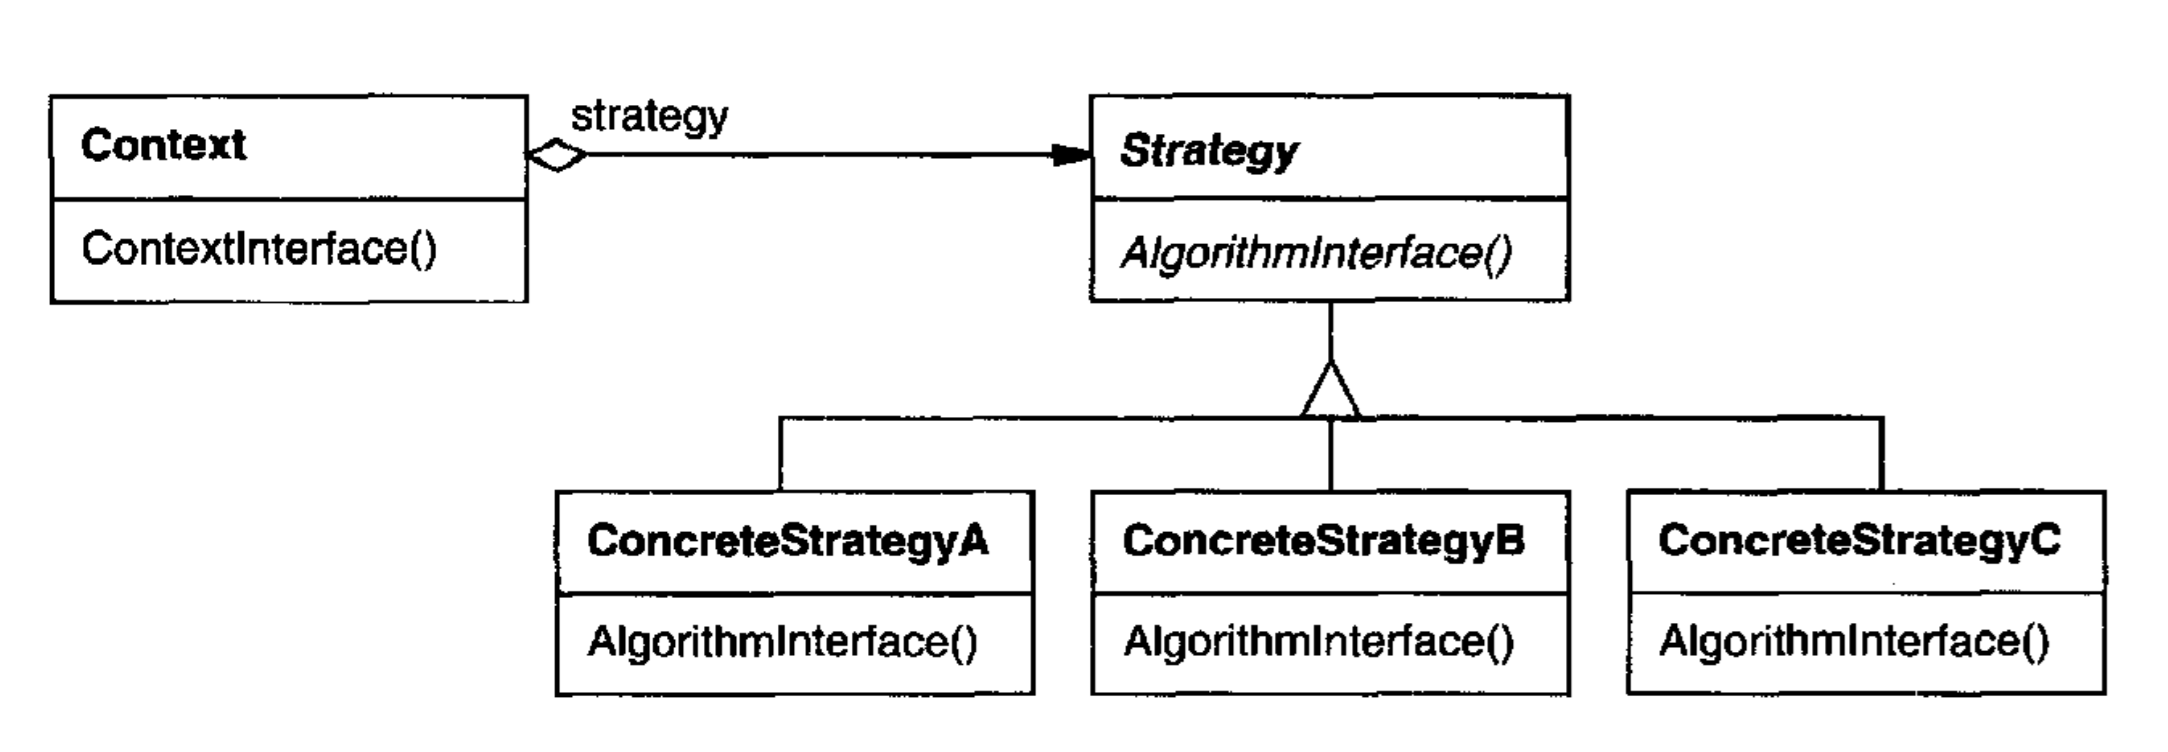
\includegraphics[width=\linewidth]{./figures/program/strategy.png}
  \caption{UML diagram for the Strategy design pattern from~\cite{DesignPatterns}}
\end{figure}

This is a great design pattern for research purposes since it facilitates experimentation with various algorithms for the same purpose. It also makes the code easily readable, as the Strategy interface provides an abstraction layer between the Context and the concrete implementation.

\subsection{Language choice}

With the specified goals and the architecture in mind, I needed a language that is object-oriented, easily readable by beginners and has extensive capabilities for using complex numbers, linear algebra and plotting. For these purposes, I choose the Python language. Python is concise, it reads like pseudocode and has libraries such as NumPy, SciPy and Matplotlib, and so on, covering all areas of data science. Furthermore, it is well-known and extensively used by researchers with no software engineering background, allowing for easier collaboration.

\subsection{High level design}

The source code of the software can be divided into three parts:

\begin{itemize}
    \item Graph models
    \item Simulators
    \item Running, configuration and result collection
\end{itemize}

\begin{figure}[H]
  
\includegraphics[width=\linewidth]{./figures/program/uml.png}
  \caption{UML diagram for the Graph models and Simulators}
\end{figure}

On the UML diagram above, the SubGraph class is a Strategy, with the following ConcreteStrategy implementations:

\begin{itemize}
    \item BinaryTree
    \item Bipartite
    \item Circle
    \item Grid
    \item Hypercube
    \item Path
    \item Random
\end{itemize}

Each of these employs an oracle that calculates neighbouring vertices on-the-fly.

Furthermore, the Simulator is also a Strategy, implemented by the Classical and the Quantum classes, the latter using the Coin Strategy, implemented by the Hadamard, Grover and Fourier (DFT) classes.

(For a cleaner diagram, I did not picture the SubGraph and Coin implementations.)

\subsection{Graph models}

I ran several experiments on various graphs while researching quantum graph walks, including paths, circles, bipartite graphs, hypercubes, and grids. Initially, I directly generated and stored their adjacency matrices, however, I quickly ran into memory scaling issues with this approach. Furthermore, in quantum research, graphs are typically built like 'Legos', glueing together a few common types, which was challenging to do with my original approach.

To combat these issues, I switched from the adjacency matrix representation to the oracle representation. The oracle is a function that returns the neighbours of a given vertex. Since I was using common graphs, I could calculate neighbouring indexes on-the-fly without storing anything about these graphs and only querying what is needed at the current step, dramatically reducing the memory requirements of the graph models.

\subsection{Simulators}

I implemented a classical and a quantum simulator class. The quantum simulator can currently simulate directed $k$ regular graphs, however since the permutation matrix decomposition, or in the undirected case, the edge coloring of the matrix is an NP-complete problem, in the current setup, the graph oracle must be implemented in a way that returns the neighbours in the same color order for all inputs. Since the human programmer designs the oracle, this is not a critical limitation at the moment. I have implemented a check as a safety guard to ensure the resulting shift matrices are unitary in case an error is made while coding one of the oracles.

\subsection{Running, configuration and result collection}

Using the above classes, I developed a framework in which experimental runs can be configured very quickly. The results of the run are collected in an aggregated Latex document, using Matplotlib for creating various graphics. It contains the given graph, the named type of the subgraphs, the adjacency matrices, the distribution results of the simulations, including empirical hitting and mixing times and the eigenvalues and eigenvectors of the evolution operators. In the following chapter, I present several examples collected from these Latex reports of my experiments.

\subsection{Availability}

My simulator software is available under the open-source MIT license on my personal Github account, under the following link:

\url{https://github.com/nemkin/quantum}

\section{Presentation of poperties of quantum walks}

In this chapter, I review classical and quantum walking on three specific graphs, for which interesting results can be observed. I discuss the evolution of the probability distributions and the hitting and mixing times for classical and quantum walks with the Hadamard, Grover and Fourier (DFT) coins.

\subsection{Walks on the line}

The first graph to be reviewed is the line (with $100$ vertices), using the adjacency matrix below. It is important to note, that an extra edge has to be added to connect the two ends of the line (see Theorem (\ref{PermutationMatricesTheorem}) for details).

\begin{figure}[H]
\centering
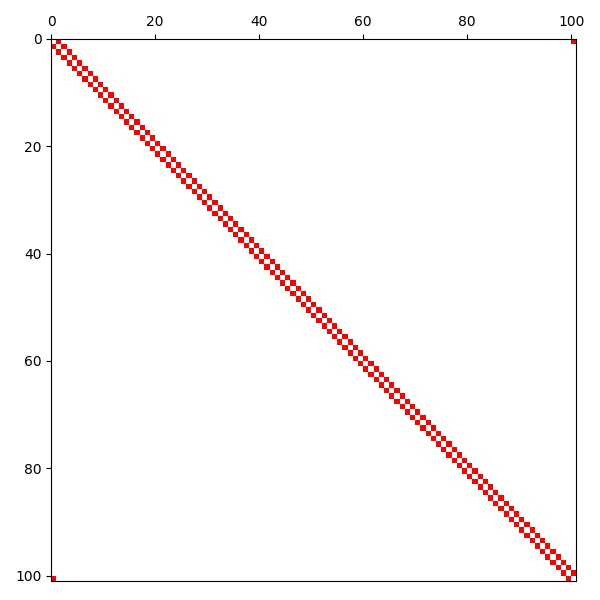
\includegraphics[width=0.5\linewidth]{./figures/results/path/graph.jpg}
\caption{Adjacency matrix of the line}
\end{figure}

In the following pictures, we can see the changes in the probability distribution during the walk. The $x$ axis contains the vertices, and the $y$ axis contains the steps. The walker starts from the centre, and in the classical case, multiple runs are done to arrive at a probability distribution, while in the quantum case, a single walker is enough, as it spreads in superposition over the graph.

The ballistic nature of the walk can be seen from steps $0$ to $50$, where the bright yellow diagonals represent a strong probability concentration spreading to the two ends of the line. When the probability bumps reach the sides, they cross over and travel to the opposite ends.

From steps $50$ to $200$, we can see secondary, tertiary, and further yellow bumps travelling alongside the main ones. These reach the ends slower and cross over each other later. This results in a beautiful weaved pattern in the picture.

Since the line is a $2$-regular graph, $2$ dimensional coins are used. The 2 dimensional Hadamard-coin and Fourier-coin are identical, while the 2 dimensional Grover-coin results in the walker not moving away from the
starting position, hence why only the Hadmard coin is shown in the distributions.

\begin{figure}[H]
  \centering
  \begin{subfigure}{.45\linewidth}
    \centering
    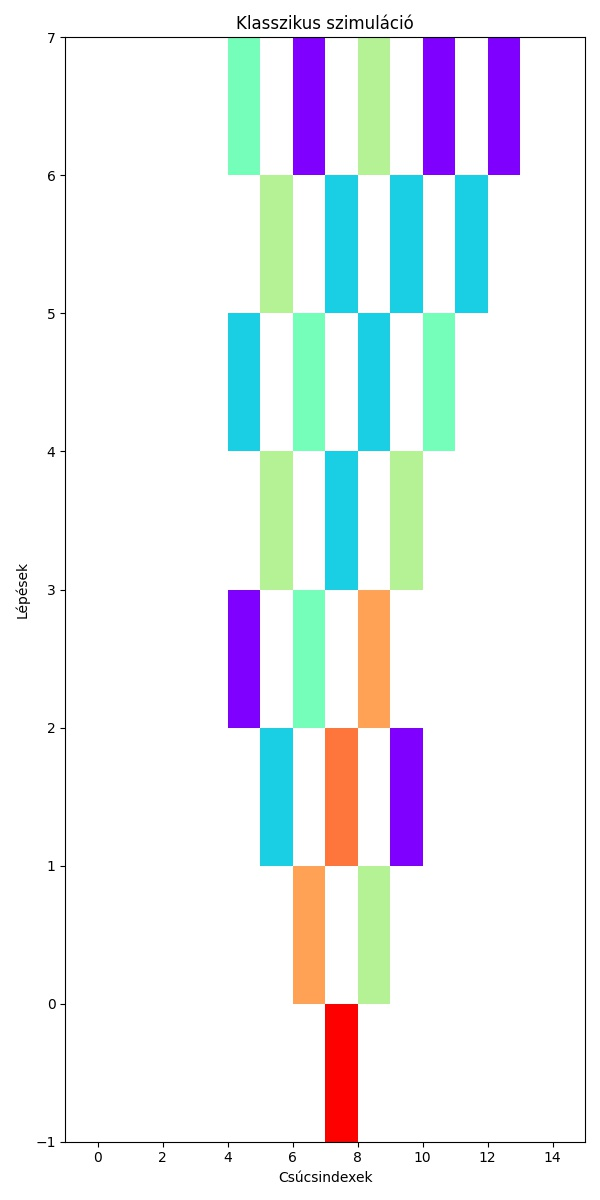
\includegraphics[width=\linewidth]{./figures/results/path/classical.jpg}
    \caption{Classical walk}
  \end{subfigure}
  \begin{subfigure}{.45\linewidth}
    \centering
    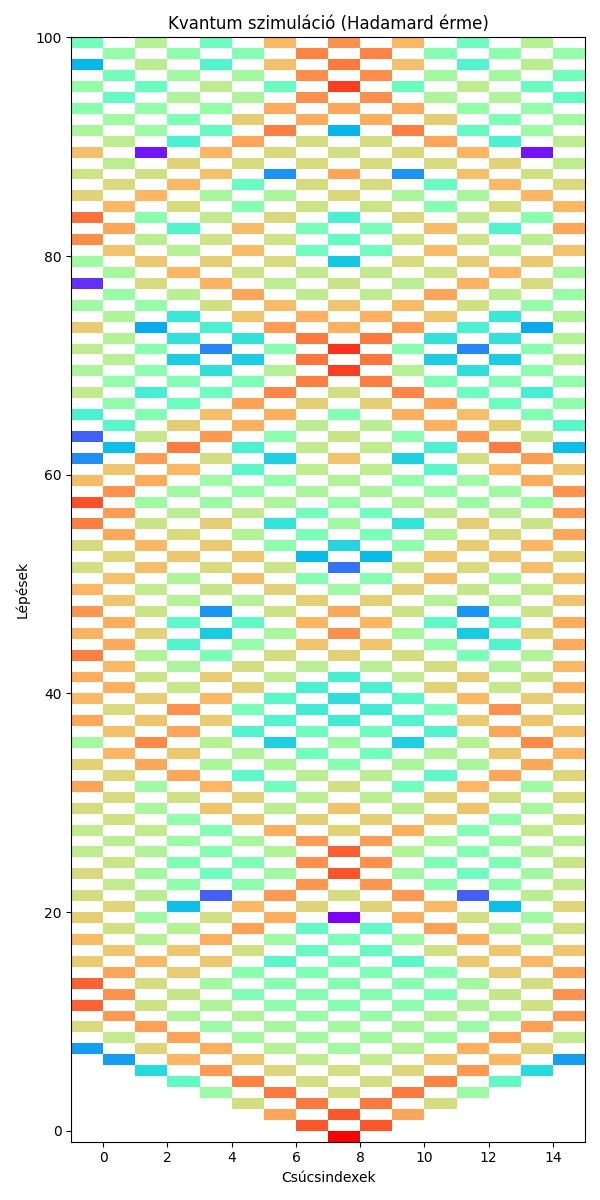
\includegraphics[width=\linewidth]{./figures/results/path/hadamard.jpg}
    \caption{Quantum walk with the Hadamard coin}
  \end{subfigure}
  \caption{Probability distribution of classical and quantum walks on the line}
\end{figure}

I have empirically measured hitting and mixing times for the different types of walks. Hitting time
is the expected number of steps to reach a specific vertex from the starting point. For this, I have
plotted the number of steps it took to first reach a particular vertex from the starting point. Mixing
time is the number of steps it takes before reaching the stationary distribution with $\varepsilon$ error.
For this, I have plotted the Euclidean difference between the walk's current and the end distribution.

In the following pictures, we can see the classical hitting and mixing times. Since my classical simulator approximates the distribution by running multiple walkers, the hitting time is slightly asymmetric. We can see from comparing the classical and the quantum hitting times that the quantum walk spreads faster than the classical one.

On the classical mixing time, we can see that the walker has not reached the stationary distribution. This is because until the walker reaches the ends of the line, the graph is essentially bipartite with two different limiting distributions and only after crossing over to the other side can the walk spread uniformly. This can also be seen in the probability distribution image above. At around step $300$, the colour of the image intensifies at the sides. Before that, the distribution alternates between odd and even indexes having $0$ probability, resulting in a chessboard pattern of white and colorful rectangles.

The quantum walk is mixing much better, as can be seen by the mixing time and the distribution image as well.

\begin{figure}[H]
  \centering
  \begin{subfigure}{.45\linewidth}
    \centering
    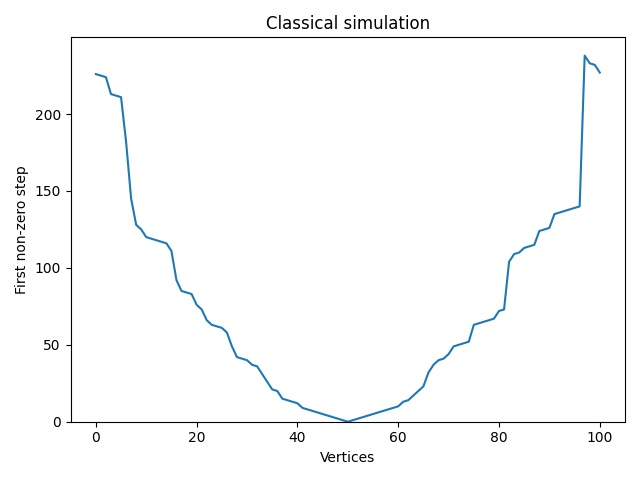
\includegraphics[width=\linewidth]{./figures/results/path/classical_hitting_time.jpg}
    \caption{Classical hitting time}
  \end{subfigure}
  \begin{subfigure}{.45\linewidth}
    \centering
    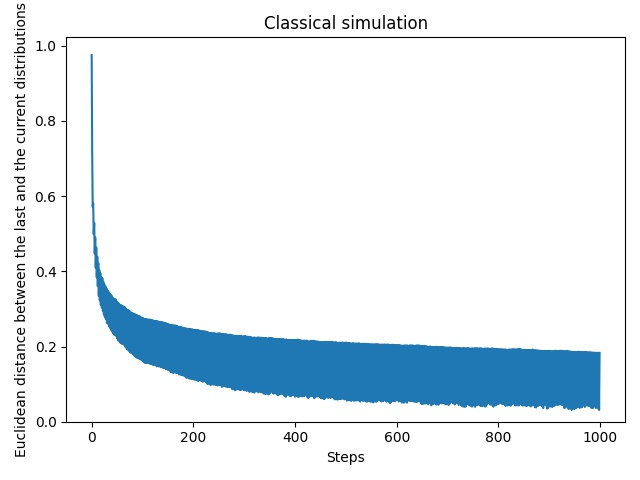
\includegraphics[width=\linewidth]{./figures/results/path/classical_mixing_time.jpg}
    \caption{Classical mixing time}
  \end{subfigure}
  \caption{Classical hitting and mixing times on the line}
\end{figure}

\begin{figure}[H]
  \centering
  \begin{subfigure}{.45\linewidth}
    \centering
    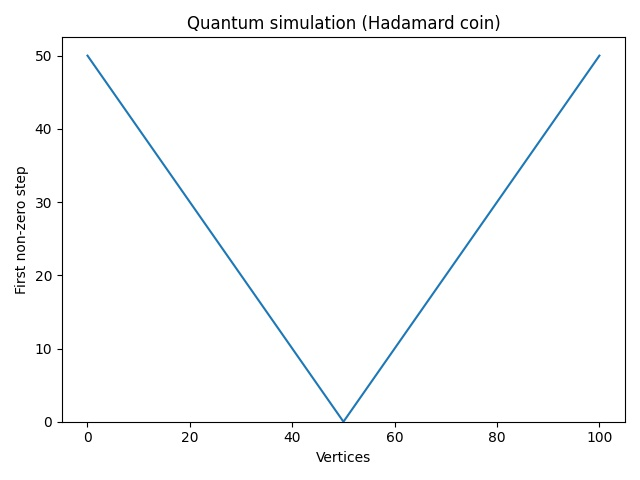
\includegraphics[width=\linewidth]{./figures/results/path/hadamard_hitting_time.jpg}
    \caption{Hadamard hitting time}
  \end{subfigure}
  \begin{subfigure}{.45\linewidth}
    \centering
    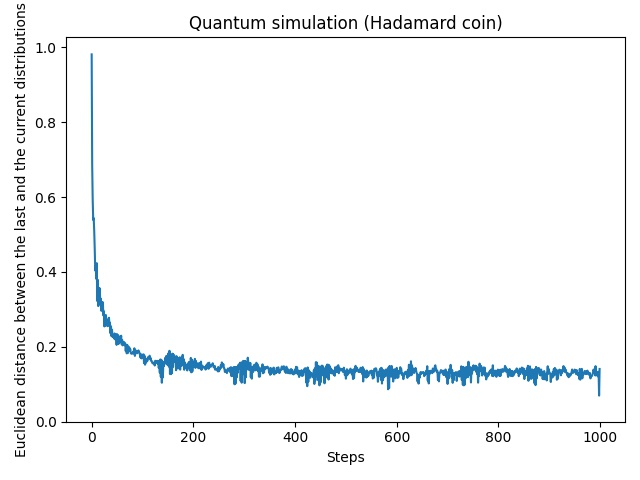
\includegraphics[width=\linewidth]{./figures/results/path/hadamard_mixing_time.jpg}
    \caption{Hadamard mixing time}
  \end{subfigure}
  \caption{Quantum (Hadamard) hitting and mixing times on the line}
\end{figure}

\subsection{Walks on the grid}

The second graph reviewed is the 2 dimensional grid (with $4\times{}4=16$ vertices), using the adjacency matrix below.

\begin{figure}[H]
\centering
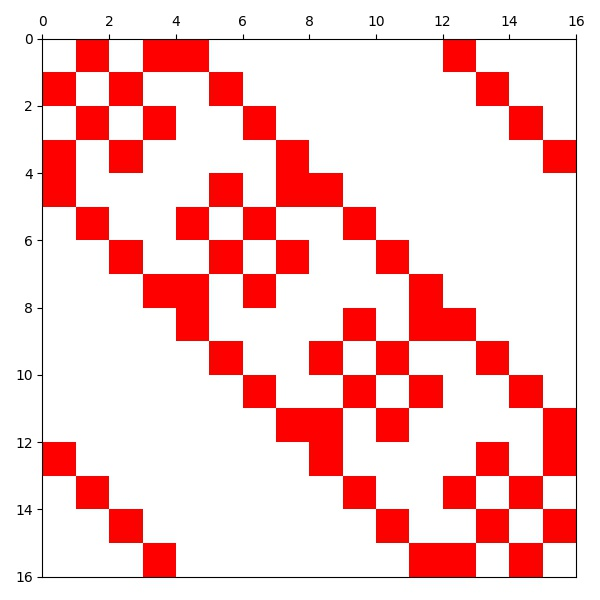
\includegraphics[width=0.5\linewidth]{./figures/results/grid/graph.jpg}
\caption{Adjacency matrix of the grid}
\end{figure}

The following 4 images contain the classical, the quantum Hadamard, the quantum Grover and the quantum Fourier walks on the grid. The classical walk quickly spreads over the graph since all vertices are close to each other (as opposed to the line, where the maximum distance is large).

In the quantum case, using the Hadamard and Grover coins, an important quality of the quantum walks can be distinctly observed: quantum walks are periodic since the eigenvalues of the evolution operator are complex roots of unity. Furthermore, by choosing a vertex count that is a power of $2$, I was able to create an evolution operator that has specific eigenvalues that result in the walker returning to its starting position
with $100\%$ probability (see the repeated red rectangles in the images), showing the cyclic nature of the quantum walk.

The Fourier coin mixes the state much better, resulting in no specific order in that image.

\begin{figure}[H]
  \centering
  \begin{subfigure}{.45\linewidth}
    \centering
    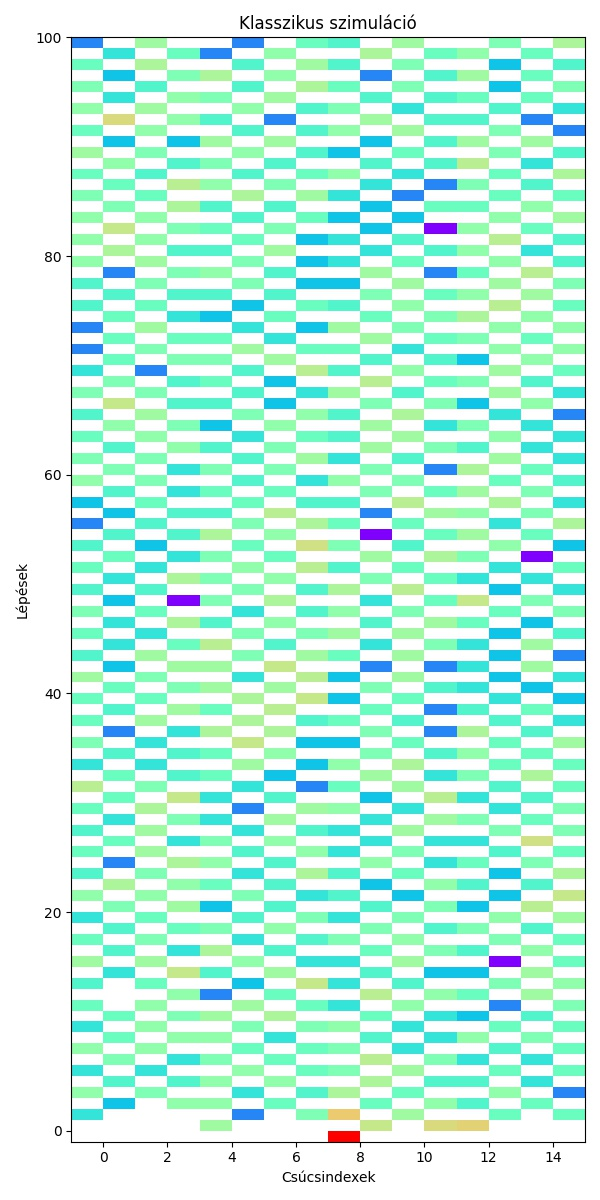
\includegraphics[width=\linewidth]{./figures/results/grid/classical.jpg}
    \caption{Classical walk}
  \end{subfigure}
  \begin{subfigure}{.45\linewidth}
    \centering
    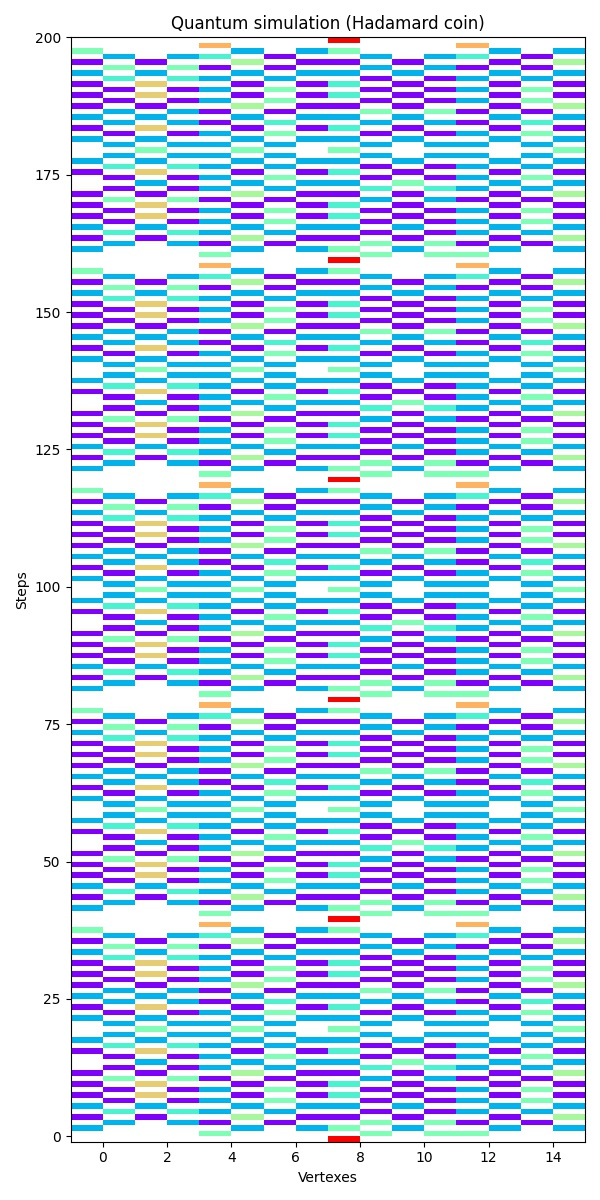
\includegraphics[width=\linewidth]{./figures/results/grid/hadamard.jpg}
    \caption{Quantum walk with the Hadamard coin}
  \end{subfigure}
  \caption{Probability distribution of classical and quantum walks on the grid}
\end{figure}

\begin{figure}[H]
  \centering
  \begin{subfigure}{.45\linewidth}
    \centering
    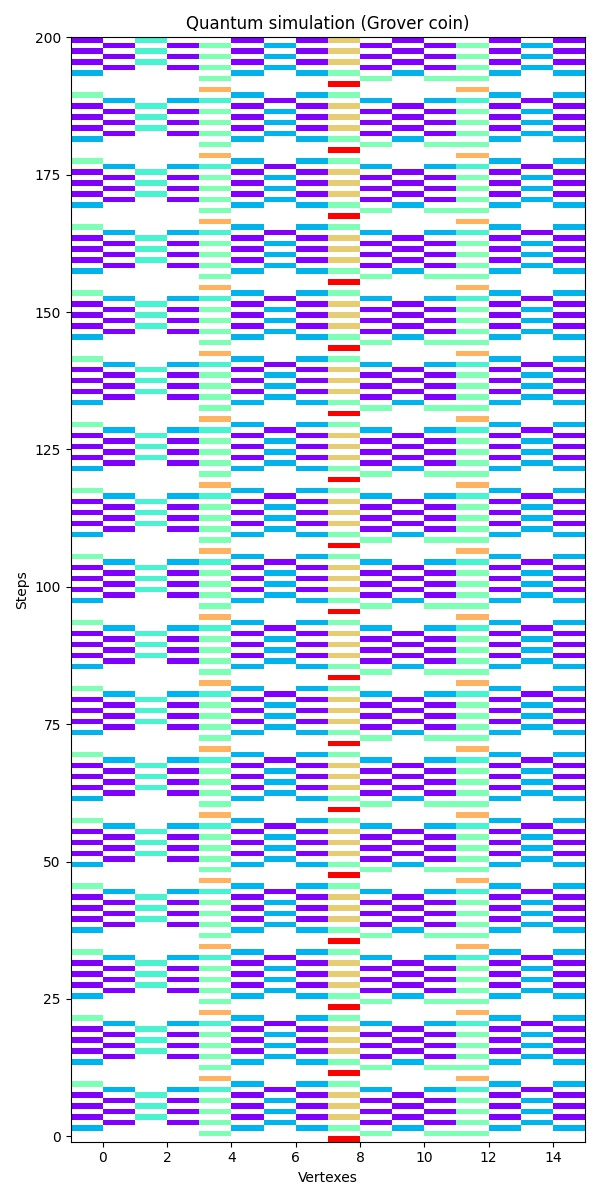
\includegraphics[width=\linewidth]{./figures/results/grid/grover.jpg}
    \caption{Quantum walk with the Grover coin}
  \end{subfigure}
  \begin{subfigure}{.45\linewidth}
    \centering
    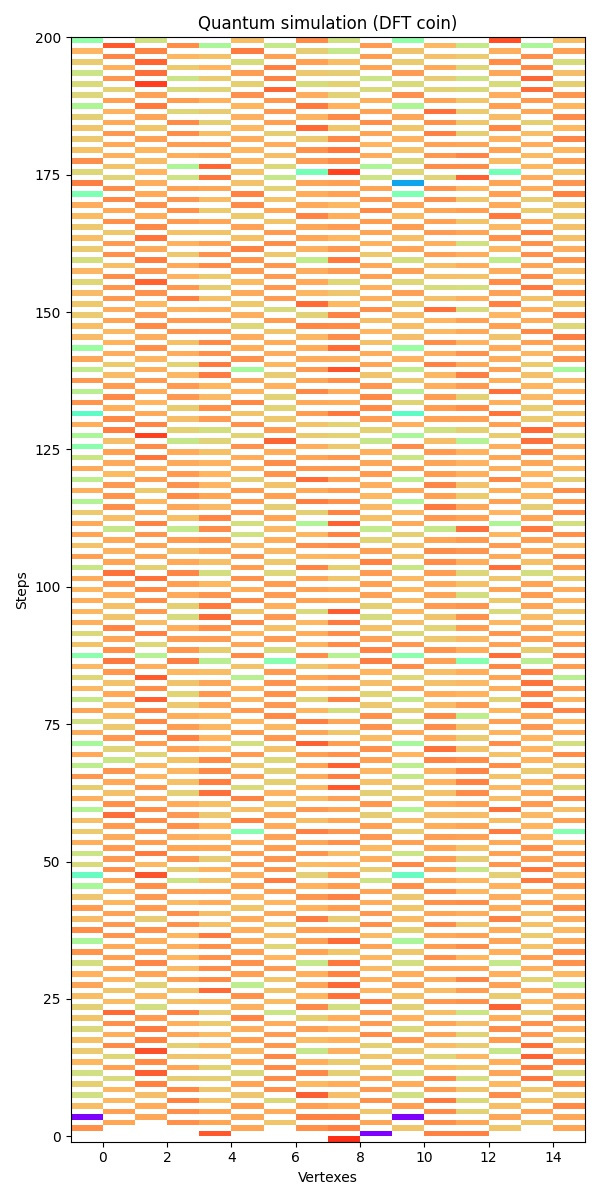
\includegraphics[width=\linewidth]{./figures/results/grid/dft.jpg}
    \caption{Quantum walk with the Fourier coin}
  \end{subfigure}
  \caption{Probability distribution of quantum walks on the grid}
\end{figure}

Interestingly, the hitting times of the 4 walks are similar. This is probably due to the fact, that the
graph is small, which allows the classical walk to spread just as quickly as its quantum counterpart. We can see, that neither of the walks reached a stationary distribution. In the quantum case, we know that the walks
are periodic, so there is no stationary distribution, while in the classical case, the graph is bipartite.

\begin{figure}[H]
  \centering
  \begin{subfigure}{.45\linewidth}
    \centering
    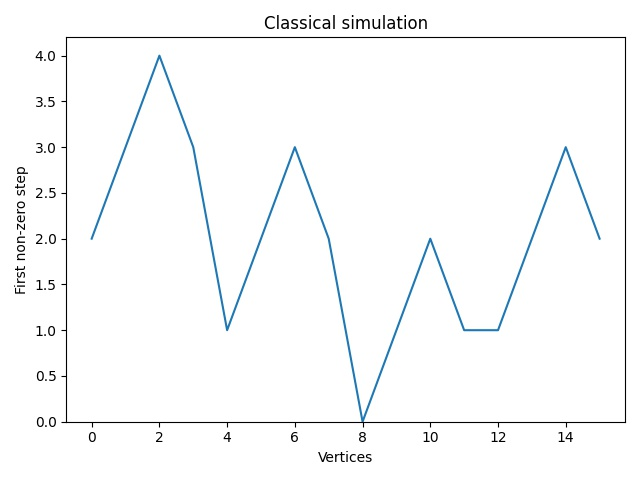
\includegraphics[width=\linewidth]{./figures/results/grid/classical_hitting_time.jpg}
    \caption{Classical hitting time}
  \end{subfigure}
  \begin{subfigure}{.45\linewidth}
    \centering
    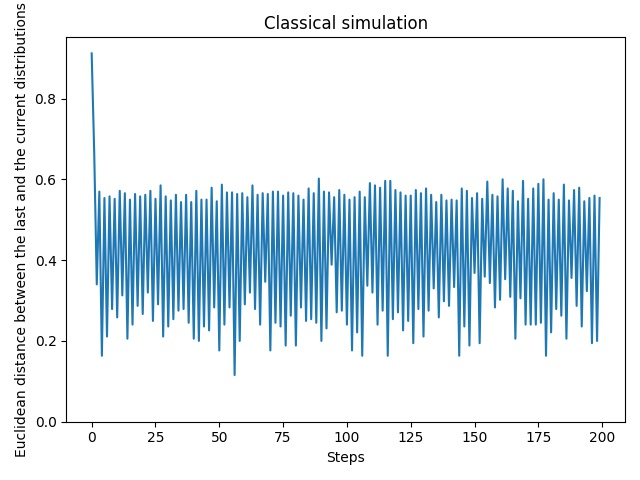
\includegraphics[width=\linewidth]{./figures/results/grid/classical_mixing_time.jpg}
    \caption{Classical mixing time}
  \end{subfigure}
  \caption{Classical hitting and mixing times on the grid}
\end{figure}

\begin{figure}[H]
  \centering
  \begin{subfigure}{.45\linewidth}
    \centering
    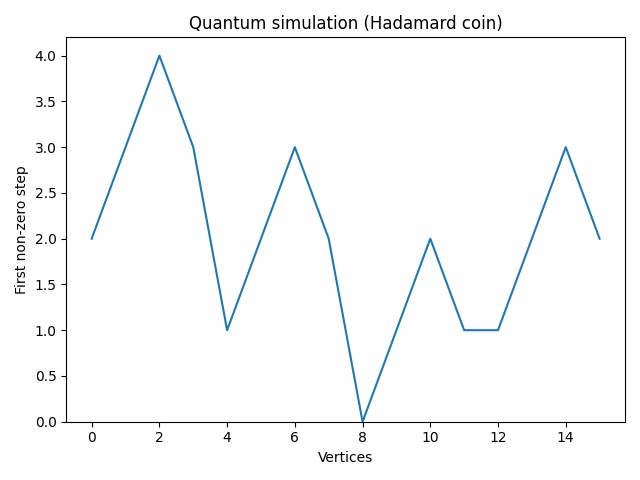
\includegraphics[width=\linewidth]{./figures/results/grid/hadamard_hitting_time.jpg}
    \caption{Hadamard hitting time}
  \end{subfigure}
  \begin{subfigure}{.45\linewidth}
    \centering
    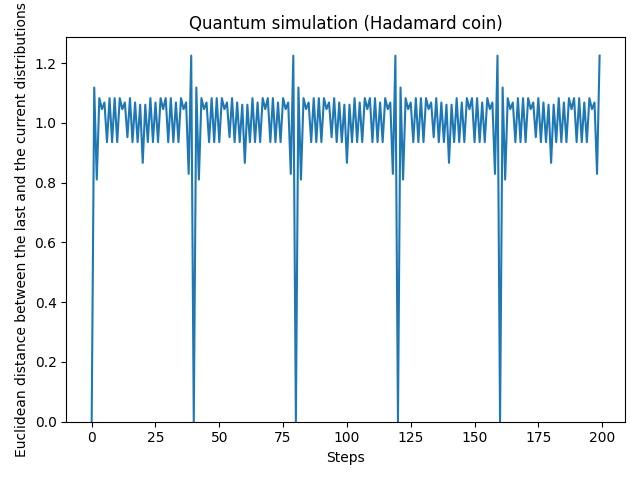
\includegraphics[width=\linewidth]{./figures/results/grid/hadamard_mixing_time.jpg}
    \caption{Hadamard mixing time}
  \end{subfigure}
  \caption{Quantum (Hadamard) hitting and mixing times on the grid}
\end{figure}

\begin{figure}[H]
  \centering
  \begin{subfigure}{.45\linewidth}
    \centering
    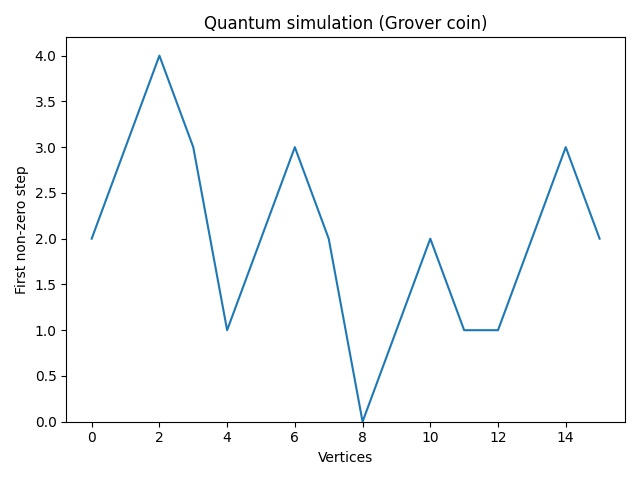
\includegraphics[width=\linewidth]{./figures/results/grid/grover_hitting_time.jpg}
    \caption{Grover hitting time}
  \end{subfigure}
  \begin{subfigure}{.45\linewidth}
    \centering
    \includegraphics[width=\linewidth]{./figures/results/grid/grover_mixing_time.jpg}
    \caption{Grover mixing time}
  \end{subfigure}
  \caption{Quantum (Grover) hitting and mixing times on the grid}
\end{figure}

\begin{figure}[H]
  \centering
  \begin{subfigure}{.45\linewidth}
    \centering
    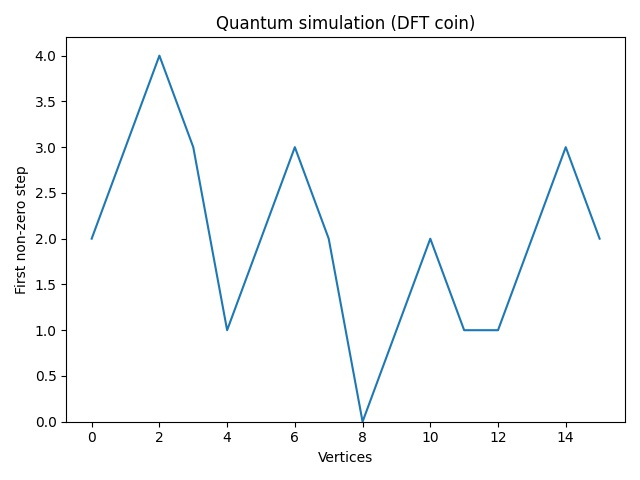
\includegraphics[width=\linewidth]{./figures/results/grid/dft_hitting_time.jpg}
    \caption{Fourier hitting time}
  \end{subfigure}
  \begin{subfigure}{.45\linewidth}
    \centering
    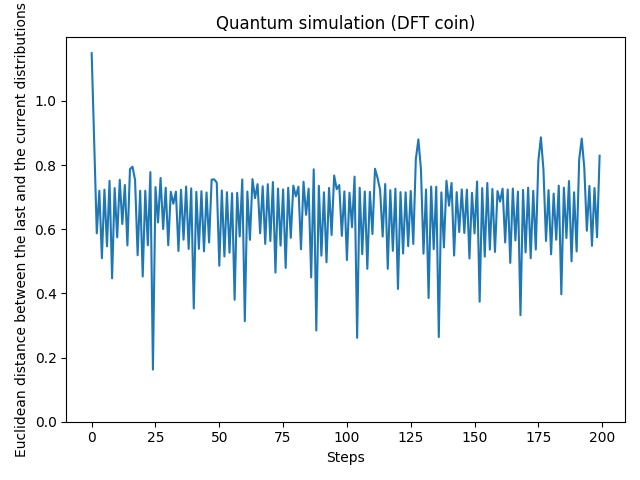
\includegraphics[width=\linewidth]{./figures/results/grid/dft_mixing_time.jpg}
    \caption{Fourier mixing time}
  \end{subfigure}
  \caption{Quantum (Fourier) hitting and mixing times on the grid}
\end{figure}

\subsection{Walks on hypercube}

The third graph reviewed is the 4 dimensional boolean hypercube (with $2^4 = 16$ vertices), using the adjacency matrix below.

\begin{figure}[H]
\centering
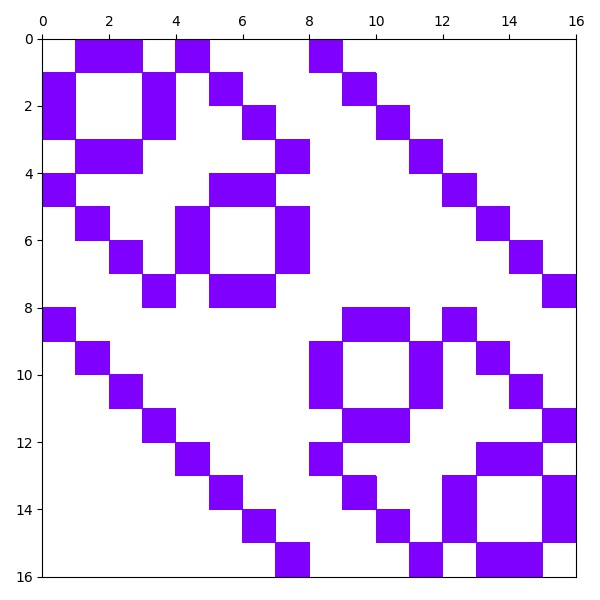
\includegraphics[width=0.5\linewidth]{./figures/results/hypercube/graph.jpg}
\caption{Adjacency graph of the hypercube}
\end{figure}

Similarly to the grid, the walks are recurrent (cyclic) in the Hadamard and Grover case. Interestingly in this case the periodicity can be visibly observed with the Fourier coin, however the walk does not return to its
original starting point with $100\%$ probability. This is due to the eigenvalues of the evolution operator
just being slightly off, so there is no small exponent for which the evolution operator is the identity.

\begin{figure}[H]
  \centering
  \begin{subfigure}{.45\linewidth}
    \centering
    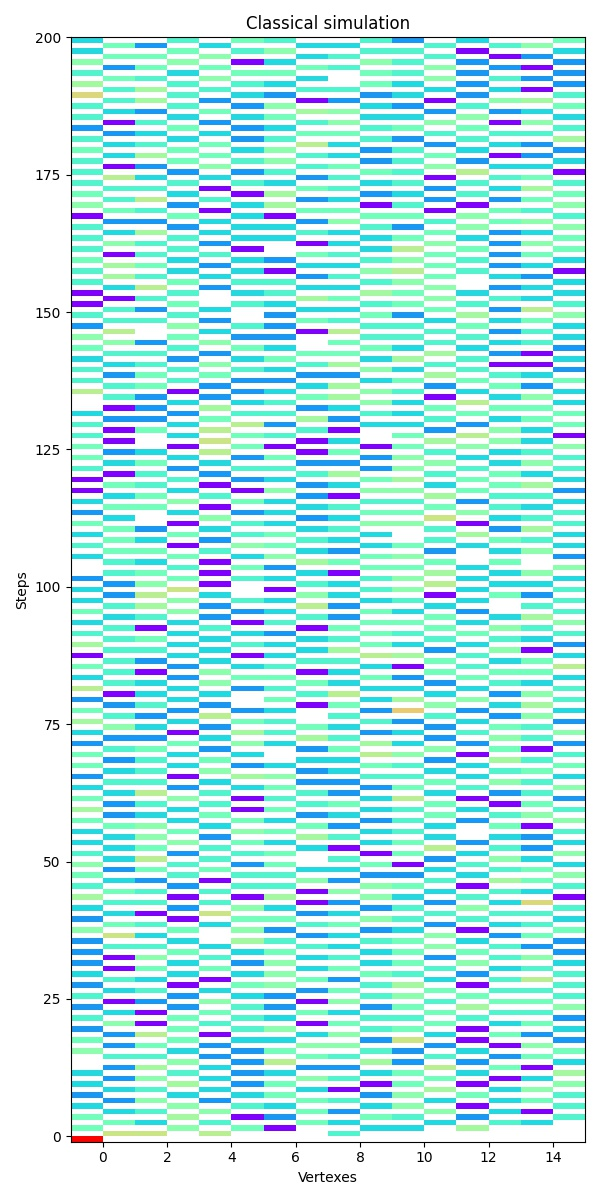
\includegraphics[width=\linewidth]{./figures/results/hypercube/classical.jpg}
    \caption{Classical walk}
  \end{subfigure}
  \begin{subfigure}{.45\linewidth}
    \centering
    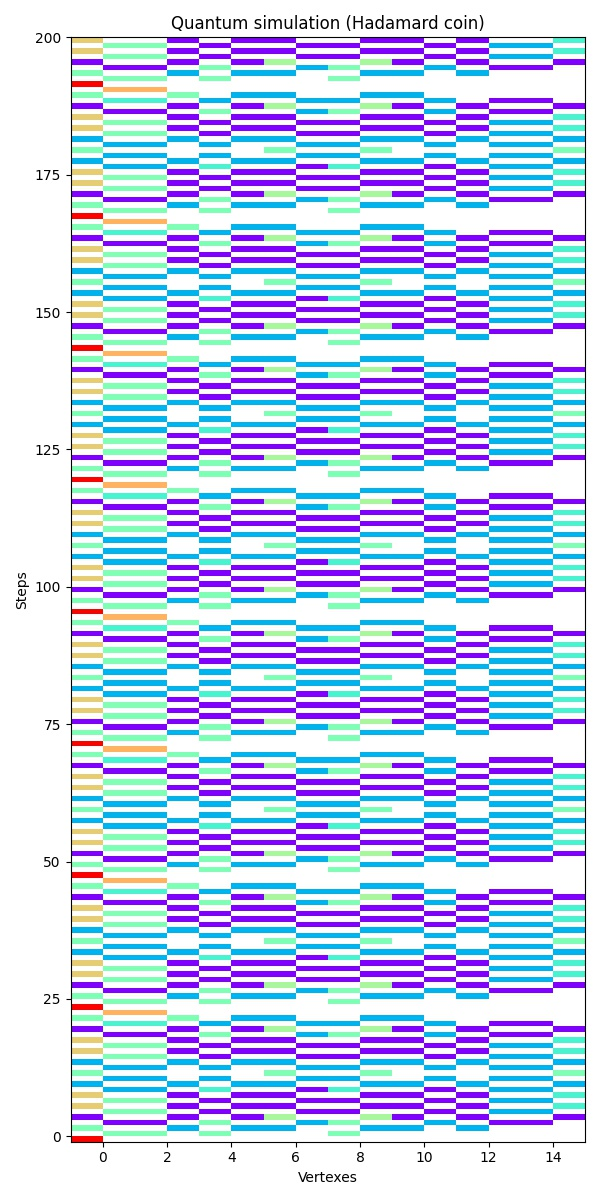
\includegraphics[width=\linewidth]{./figures/results/hypercube/hadamard.jpg}
    \caption{Quantum walk with the Hadamard coin}
  \end{subfigure}
  \caption{Probability distribution of classical and quantum walks on the hypercube}
\end{figure}

\begin{figure}[H]
  \centering
  \begin{subfigure}{.45\linewidth}
    \centering
    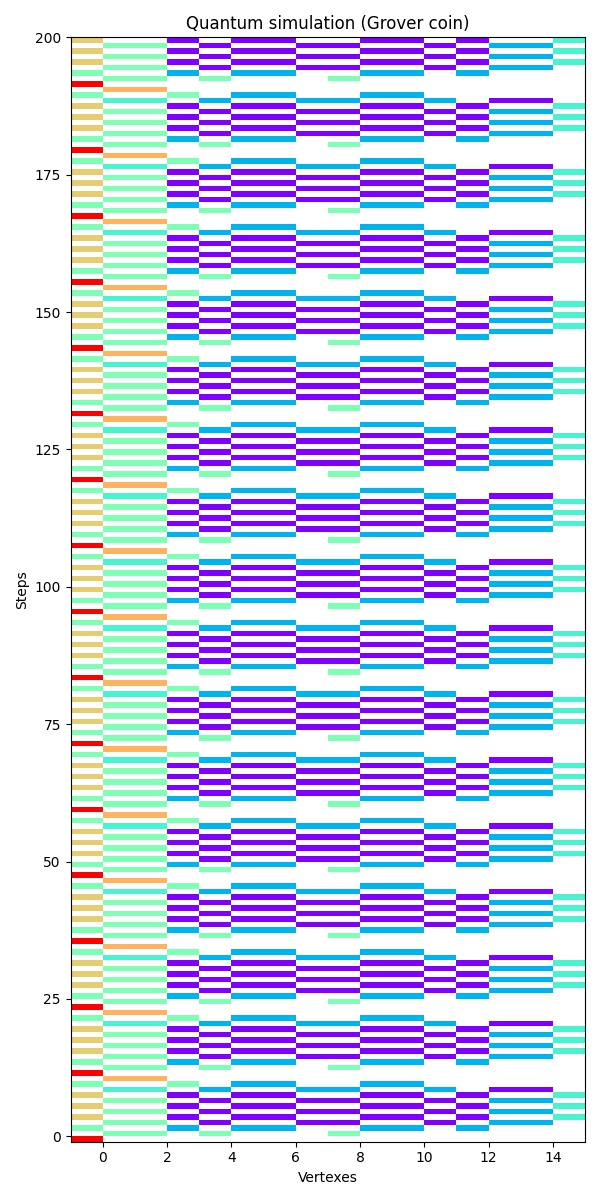
\includegraphics[width=\linewidth]{./figures/results/hypercube/grover.jpg}
    \caption{Quantum walk with the Grover coin}
  \end{subfigure}
  \begin{subfigure}{.45\linewidth}
    \centering
    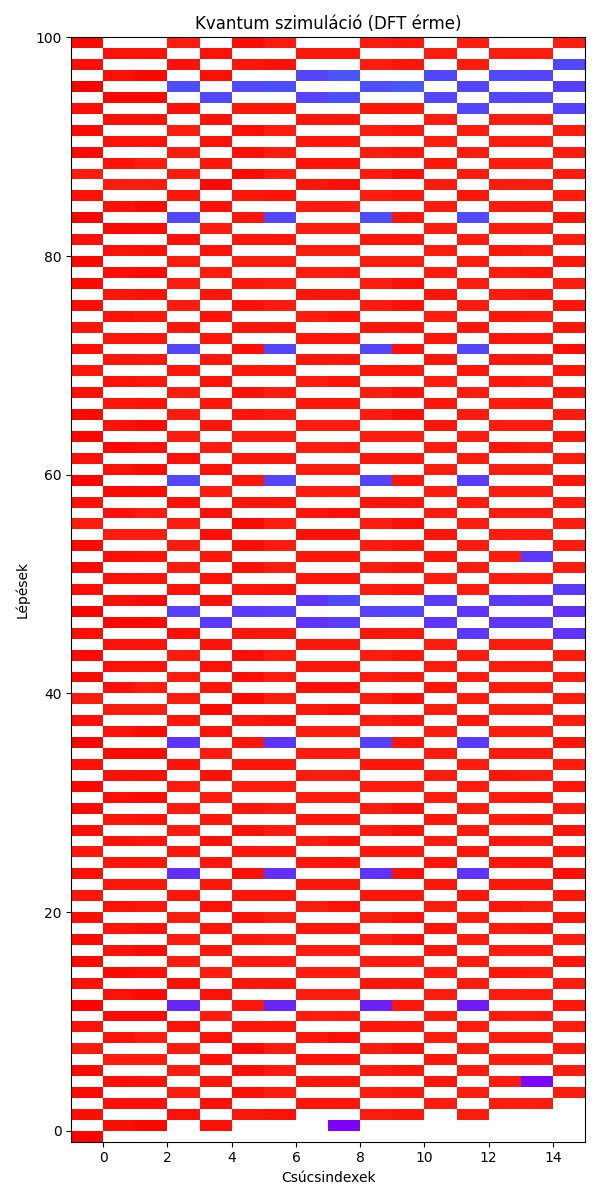
\includegraphics[width=\linewidth]{./figures/results/hypercube/dft.jpg}
    \caption{Quantum walk with the Fourier coin}
  \end{subfigure}
  \caption{Probability distribution of quantum walks on the hypercube}
\end{figure}

Similarly to the grid, the hitting times are identical, since the graph is small and the classical walk's
disadvantage is not visible. The hypercube is also bipartite, resulting in no stationary distribution for the
classical walk either.

\begin{figure}[H]
  \centering
  \begin{subfigure}{.45\linewidth}
    \centering
    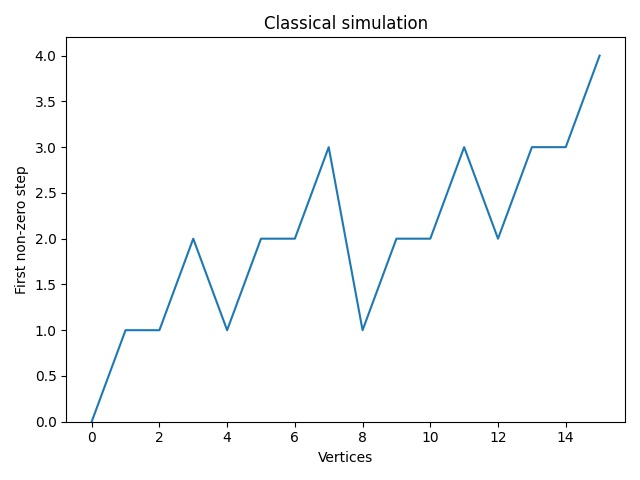
\includegraphics[width=\linewidth]{./figures/results/hypercube/classical_hitting_time.jpg}
    \caption{Classical hitting time}
  \end{subfigure}
  \begin{subfigure}{.45\linewidth}
    \centering
    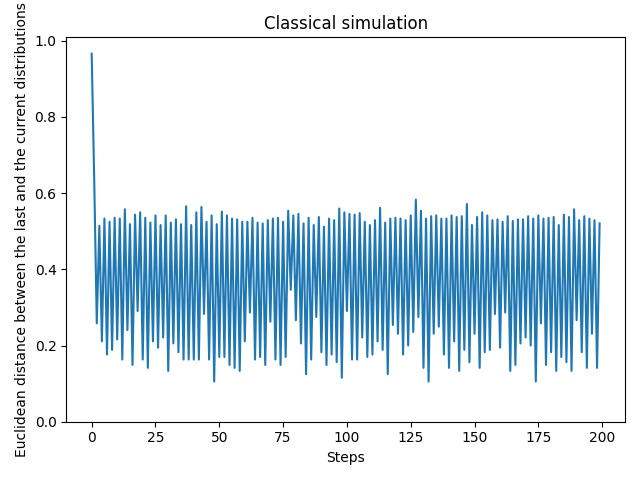
\includegraphics[width=\linewidth]{./figures/results/hypercube/classical_mixing_time.jpg}
    \caption{Classical mixing time}
  \end{subfigure}
  \caption{Classical hitting and mixing times on the hypercube}
\end{figure}

\begin{figure}[H]
  \centering
  \begin{subfigure}{.45\linewidth}
    \centering
    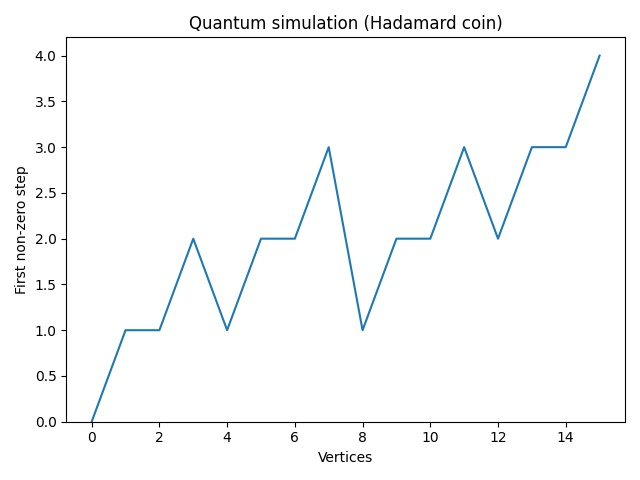
\includegraphics[width=\linewidth]{./figures/results/hypercube/hadamard_hitting_time.jpg}
    \caption{Hadamard hitting time}
  \end{subfigure}
  \begin{subfigure}{.45\linewidth}
    \centering
    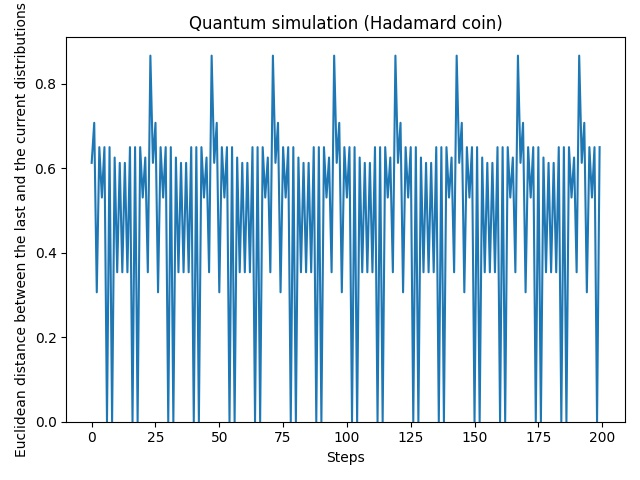
\includegraphics[width=\linewidth]{./figures/results/hypercube/hadamard_mixing_time.jpg}
    \caption{Hadamard mixing time}
  \end{subfigure}
  \caption{Quantum (Hadamard) hitting and mixing times on the hypercube}
\end{figure}

\begin{figure}[H]
  \centering
  \begin{subfigure}{.45\linewidth}
    \centering
    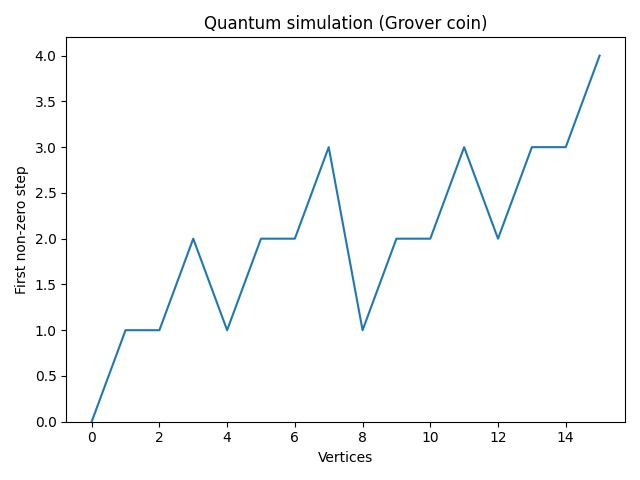
\includegraphics[width=\linewidth]{./figures/results/hypercube/grover_hitting_time.jpg}
    \caption{Grover hitting time}
  \end{subfigure}
  \begin{subfigure}{.45\linewidth}
    \centering
    \includegraphics[width=\linewidth]{./figures/results/hypercube/grover_mixing_time.jpg}
    \caption{Grover mixing time}
  \end{subfigure}
  \caption{Quantum (Grover) hitting and mixing times on the hypercube}
\end{figure}

\begin{figure}[H]
  \centering
  \begin{subfigure}{.45\linewidth}
    \centering
    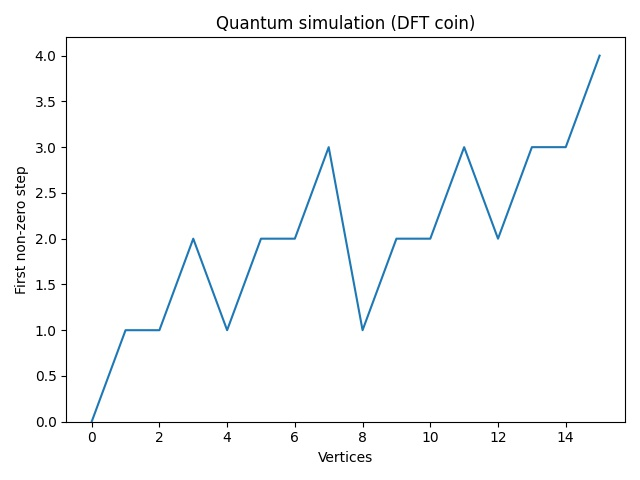
\includegraphics[width=\linewidth]{./figures/results/hypercube/dft_hitting_time.jpg}
    \caption{Fourier hitting time}
  \end{subfigure}
  \begin{subfigure}{.45\linewidth}
    \centering
    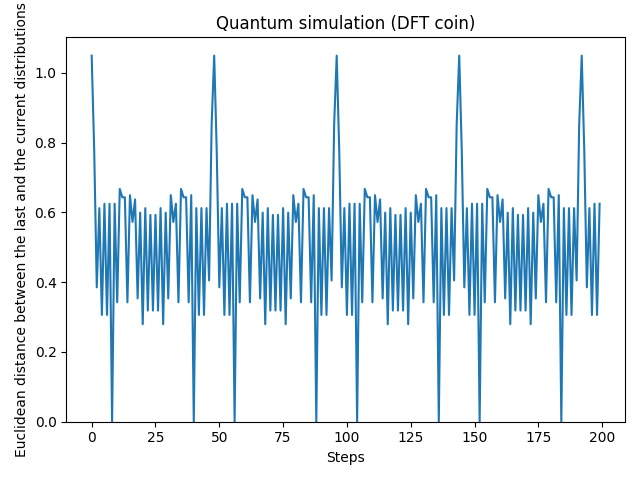
\includegraphics[width=\linewidth]{./figures/results/hypercube/dft_mixing_time.jpg}
    \caption{Fourier mixing time}
  \end{subfigure}
  \caption{Quantum (Fourier) hitting and mixing times on the hypercube}
\end{figure}

\chapter{Grover's quantum search algorithm}

Grover's search algorithm\cite{GroverOriginal} is a quantum algorithm framework, that takes a user-defined solution verifier algorithm (the oracle) and turns it into a $\Theta(\sqrt{N})$\cite{bennett_strengths_1997} solver. This provides a quadratic speedup over the classical brute force equivalent.

\section{Introduction to Grover's search algorithm framework}

Many sources call this a database search algorithm, since in Grover's original paper it was described as such. However, the 'database' here is an abstract entity, that represents the entire domain of the problem, while the so-called 'marked' elements are the correct solutions in this domain, for which the oracle would return a 'YES' answer. Using the terms 'problem domain' instead of 'database', 'verifier algorithm' insead of 'oracle' and 'solutions' instead of 'marked elements' makes Grover's importance and connection to the P versus NP problem clearer and the details of the algorithm easier to understand.

Another common description of Grover's search algorithm is that it can solve 'unstructured search problems'. What they mean by this is that the algorithm doesn't construct a solution by iterating over partial solutions or improving a non-solution step-by-step. Constrast this with for example how Prim's minimum spanning tree algorithm iterates on partial solutions by connecting the remaining vertices of the graph one at a time. This requires knowledge of the graph and knowledge of how to build a minimal spanning tree one vertex at a time.

Grover doesn't need to know the structure of the original problem, the relationship between partial solutions or how to improve non-solutions. It only needs to know how to verify a solution. It starts by taking all of the entities from the problem's domain with uniform distribution.

\begin{figure}[H]
    \centering
    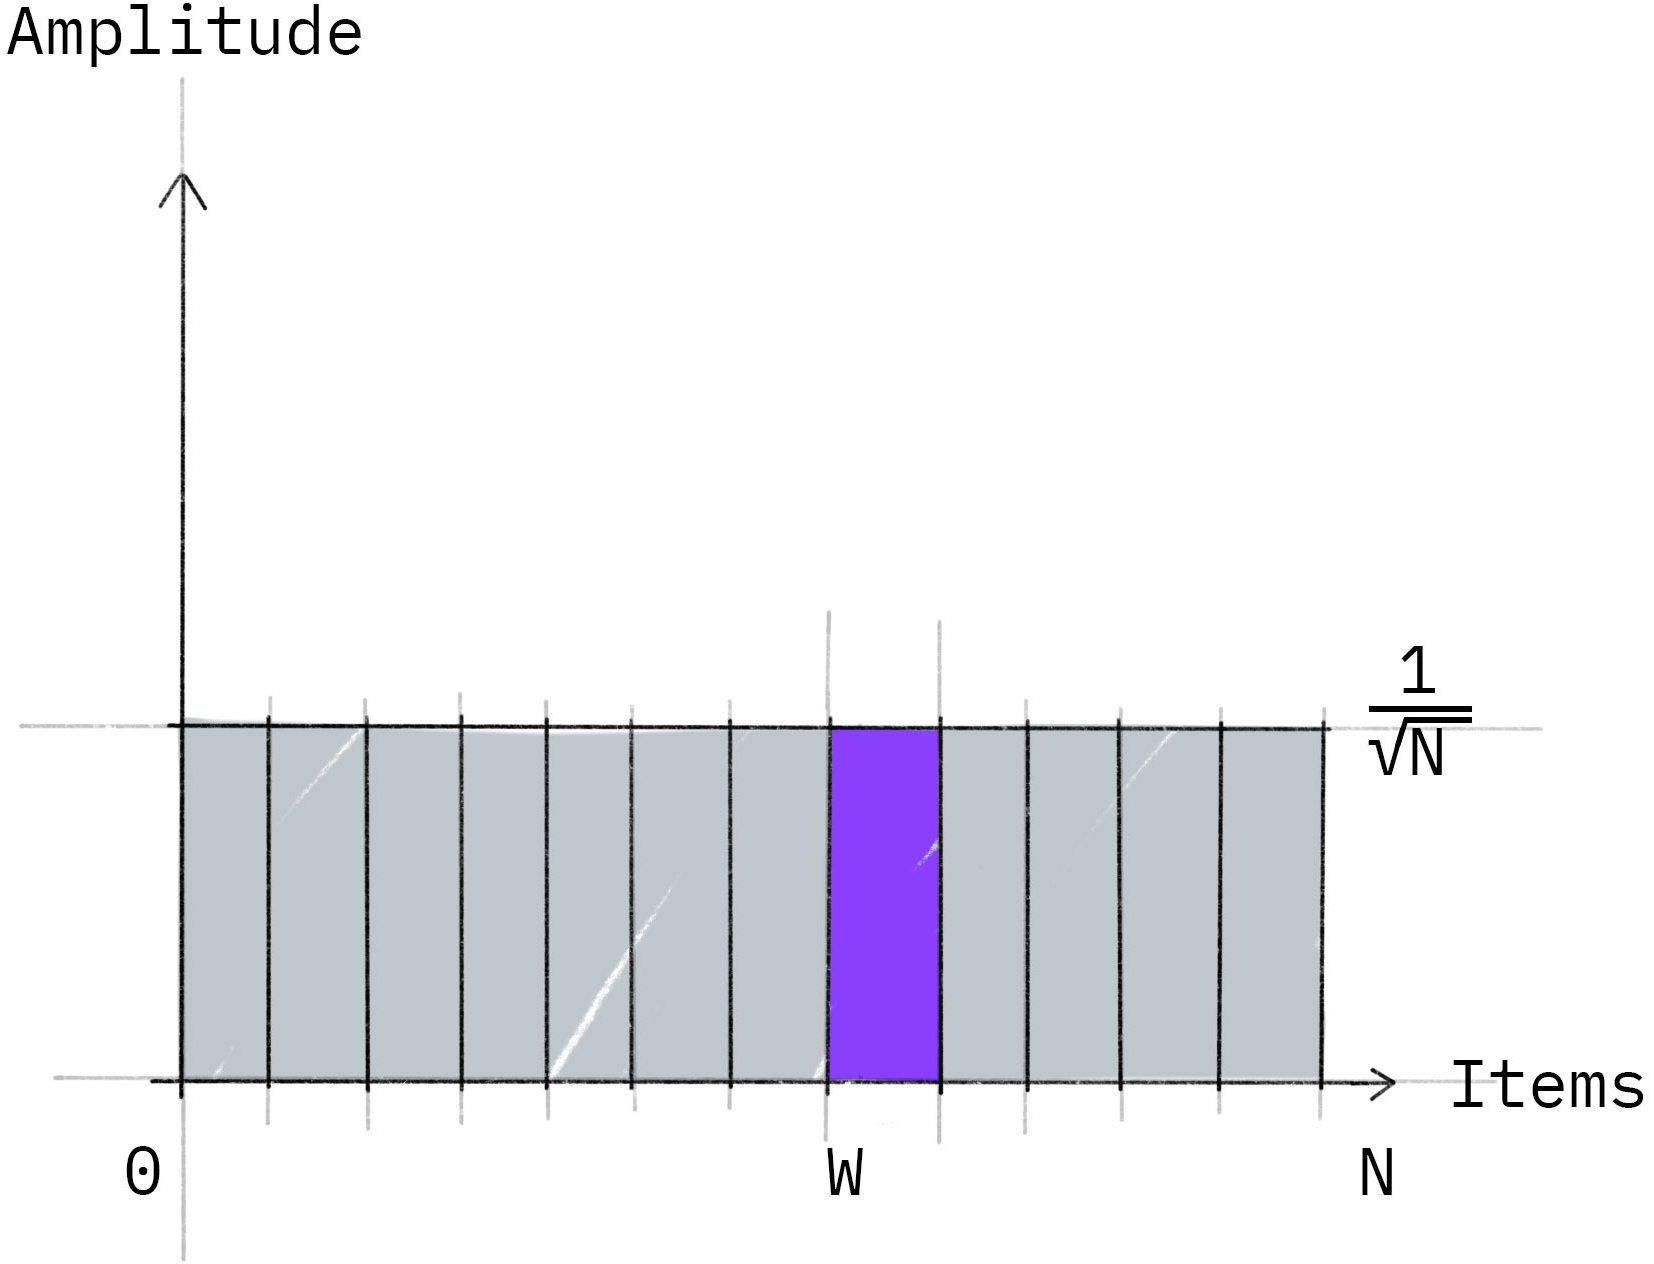
\includegraphics[width=0.5\linewidth]{content/assets/03_grovers_algorithm/grover_uniform.jpg}
    \caption{Grover starts out with the uniform distribution\cite{GroverQiskitTextbook}}
\end{figure}

Then, it uses the verifier algorithm in a process to manipulate their probabilities until the correct entities' probabilities are very high, while the incorrect entities' probabilities are very low. This process is called amplitude amplification.

\begin{figure}[H]
    \centering
    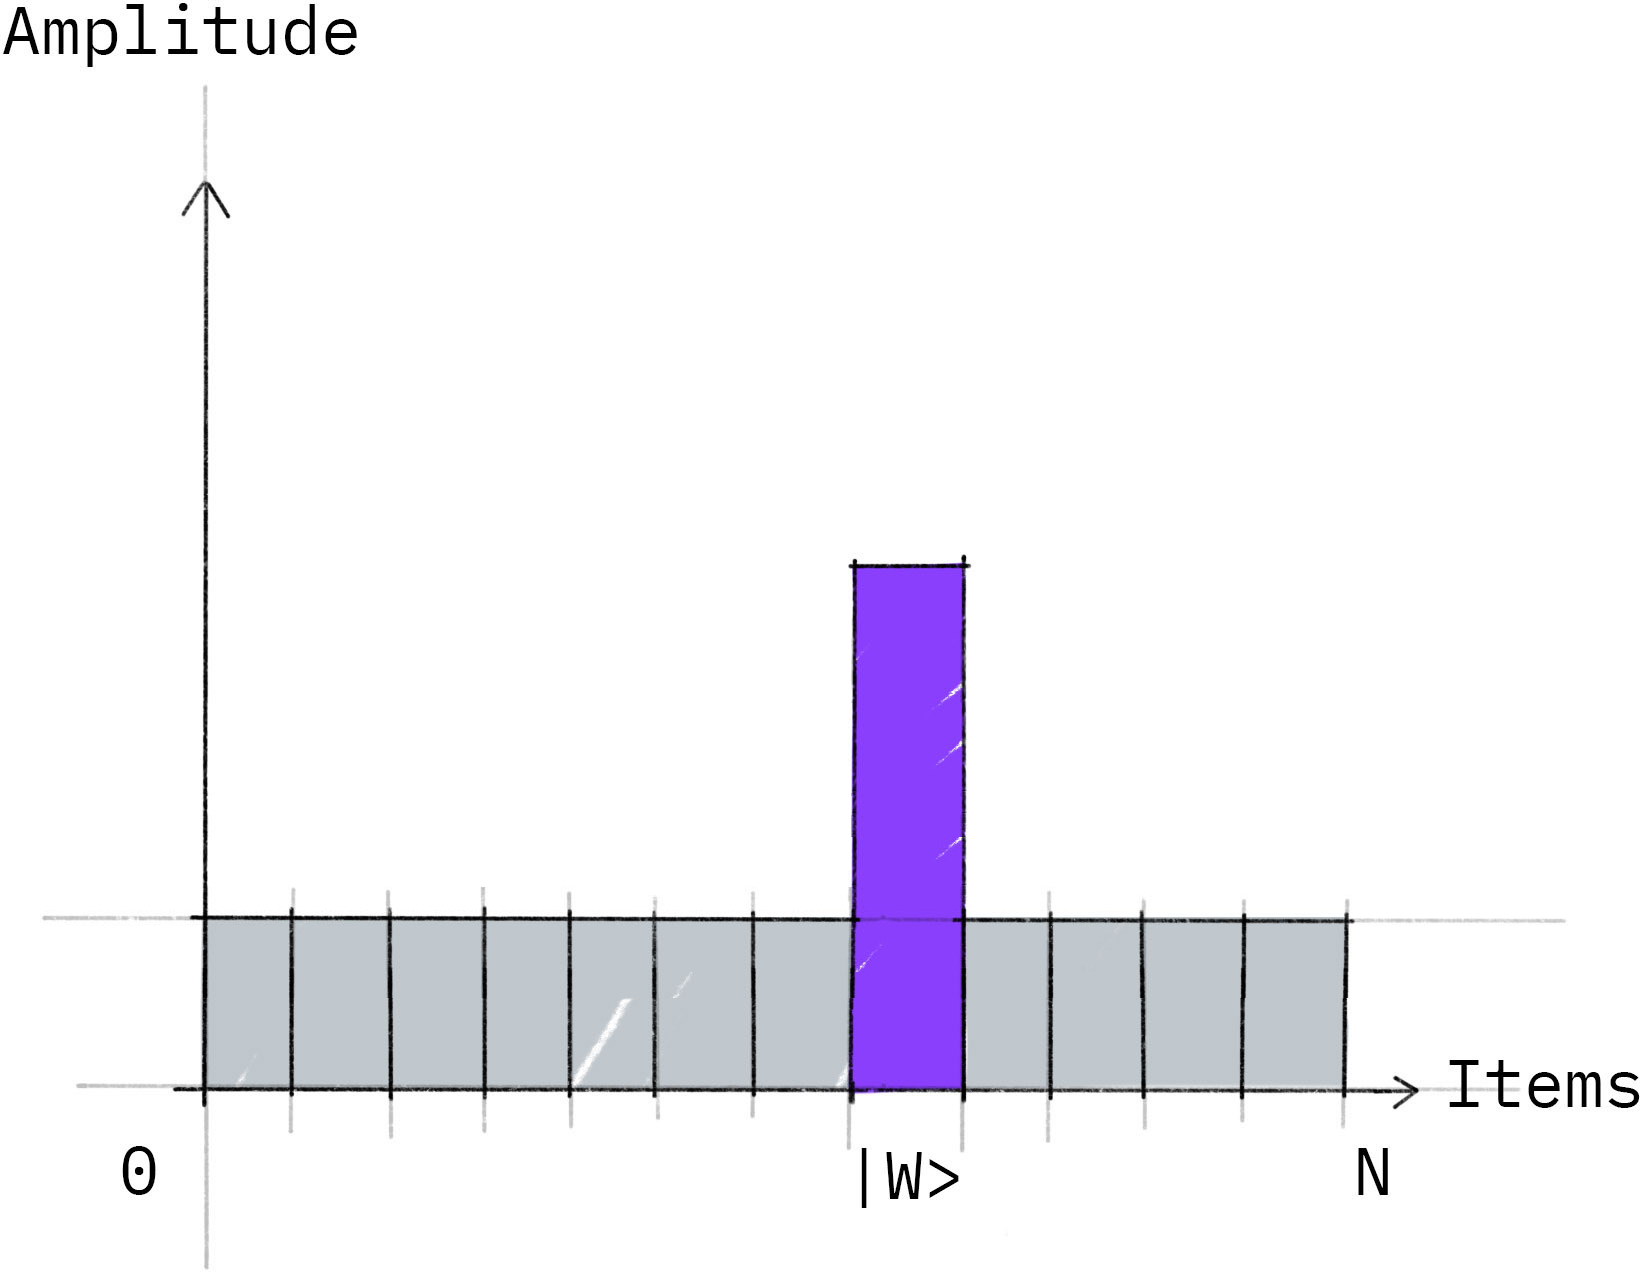
\includegraphics[width=0.5\linewidth]{content/assets/03_grovers_algorithm/grover_final.jpg}
    \caption{Grover amplifies the amplitude(s) of the correct solution(s)\cite{GroverQiskitTextbook}}
\end{figure}

Finally, it samples from this probability distribution, which results in a correct solution entity with a high chance.

Working with a probability distribution over an exponentially large set of entities is only possible in a memory-efficient way on a quantum computer, thanks to the quantum physical nature of qubits.

A register of classical bits can only represent a single entity (encoded as a binary number), we would need separate registers to represent a set and we can only operate on the entire set in a linear fashion, one register at a time. In contrast, a register of quantum bits, or 'qubits' itself can represent a set of entities (a set of binary numbers) from the domain using the quantum physical phenomenon of superposition with a probability distribution over these elements.

The manipulation of these probabilities happens using quantum operators or gates, which are the basis of all quantum algorithms on gated general-purpose quantum computers.

However, we do not have access to this probability distribution or the high probability elements in it. The only thing we can do is read the register, which is an operation that samples a single entity from the current probability distribution in the register, destroying it in the process. We are unable to 'iterate' the contents of the register or know what the probability of the resulting element was from the sampling.

This is the reason why quantum parallelism is not as trivial as the name suggests: while we can run the computation itself in parallel, gaining access to the information that we stored in the register is difficult and destructive. Amplitude amplification is a technique that we use to fix this problem, however it requires $O(\sqrt{N})$ time, where $N$ is the size of the problem's domain, where $N=2^n$ if the quantum register has $n$ qubits.

One of the most important property of quantum registers is that they can even represent probability distributions, even ones where the individual qubits are \textbf{not independent}. This is called quantum entanglement.

The simplest forms of quantum entanglement are Bell states, which can occur between two qubits. In one of these Bell states, the probability distribution of our 2 qubit quantum registers is "$00$" with $50\%$ probability and "$11$" with $50\%$. Reading the contents of just the first qubit will result in a $50\%$ chance of reading a $0$ and a $50\%$ chance of reading a $1$. However, once we know the result from the first qubit, we can be $100\%$ sure, that when we sample the second qubit, we will get the same number as a result from it.

\section{Showcasing the algorithm on a simple task}

In the original Sudoku puzzle, we have a $(3^2\cdot{}3^2)$ table, that must be filled with numbers between $1$ and $9$. A correct solution to a puzzle is where each row, column and distinct $(3\cdot{}3)$ square has unique numbers.

\begin{figure}[H]
  \centering
  \begin{subfigure}{.49\linewidth}
    \centering
    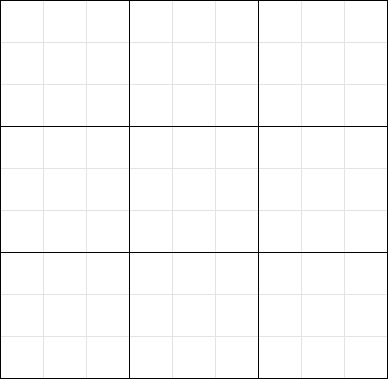
\includegraphics[width=\linewidth]{content/assets/03_grovers_algorithm/sudoku_3_empty.png}
    \caption{Empty}
  \end{subfigure}
  \begin{subfigure}{.49\linewidth}
    \centering
    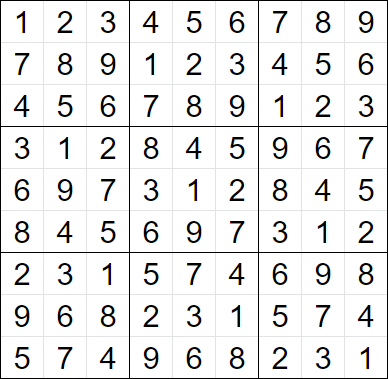
\includegraphics[width=\linewidth]{content/assets/03_grovers_algorithm/sudoku_3_solution.png}
    \caption{Solved}
  \end{subfigure}
  \caption{Sudoku puzzle}
\end{figure}

In order demonstrate memory usage scaling, I generalize this Sudoku to a table of size $(n^2\cdot{} n^2)$, where each row, column and $(n\cdot{}n)$ distinct subsquare of the table must be a unique number from the $[1, n^2]$ interval.

The only solution for $n=1$ is trivial.

\begin{figure}[H]
  \centering
  \begin{subfigure}{.4\linewidth}
  \end{subfigure}
  \begin{subfigure}{.1\linewidth}
    \centering
    
\includegraphics[width=0.6\linewidth]{content/assets/03_grovers_algorithm/sudoku_1_empty.png}
    \caption{Empty}
  \end{subfigure}
  \begin{subfigure}{.1\linewidth}
    \centering
    \includegraphics[width=0.6\linewidth]{content/assets/03_grovers_algorithm/sudoku_1_solution.png}
    \caption{Solved}
  \end{subfigure}
  \begin{subfigure}{.4\linewidth}
  \end{subfigure}
  \caption{Sudoku puzzle $(n=1)$}
\end{figure}

An example solution for $n=2$.

\begin{figure}[H]
  \centering
  \begin{subfigure}{.25\linewidth}
  \end{subfigure}
  \begin{subfigure}{.25\linewidth}
    \centering
    \includegraphics[width=\linewidth]{content/assets/03_grovers_algorithm/sudoku_2_empty.png}
    \caption{Empty}
  \end{subfigure}
  \begin{subfigure}{.25\linewidth}
    \centering
    \includegraphics[width=\linewidth]{content/assets/03_grovers_algorithm/sudoku_2_solution.png}
    \caption{Solved}
  \end{subfigure}
  \begin{subfigure}{.25\linewidth}
  \end{subfigure}
  \caption{Sudoku puzzle $(n=2)$}
\end{figure}

$n=3$ is normal Sudoku.

And an example for $n=4$ is the following.

\begin{figure}[H]
  \centering
  \begin{subfigure}{.49\linewidth}
    \centering
    \includegraphics[width=\linewidth]{content/assets/03_grovers_algorithm/sudoku_4_empty.png}
    \caption{Empty}
  \end{subfigure}
  \begin{subfigure}{.49\linewidth}
    \centering
    \includegraphics[width=\linewidth]{content/assets/03_grovers_algorithm/sudoku_4_solution.png}
    \caption{Solved}
  \end{subfigure}
  \caption{Sudoku puzzle $(n=4)$}
\end{figure}

\section{Designing a quantum solver for the Sudoku puzzle}

In this section I first define the Sudoku problem's representation in a binary form, then design the verifier algorithm (quantum oracle) for the puzzle, finally I go over the remaining parts of Grover's framework and the amplitude amplification technique it uses.

\subsection{Register definitions}

The first step is to encode the problem using quantum registers. The size-$n$ Sudoku table has $n^2$ rows and columns. Every cell in it is represented by a quantum register:

\begin{align*}
\text{cell}[i][j] = \ket{0\dots{}010\dots{}0}, & \hspace{3mm}\forall{}\hspace{1mm}(0\leq{}i,j<n^2).
\end{align*}

The length (qubits) of the register is $n^2$ and the number in the cell is represented using one-hot encoding. One-hot encoding means, that a number between $0$ and $b-1$ is represented by a $b$ bit register, each number corresponding to a single bit being $1$ in the register:

\begin{align*}
\text{cell}[i][j][k] = \begin{cases}
\ket{1} & \text{cell}_{(i,j)}\text{'s number is }(k+1) \\
\ket{0} & \text{otherwise}
\end{cases}, & \hspace{3mm}\forall{}(\hspace{1mm}0\leq{}i,j,k<n^2).
\end{align*}

In Qiskit, once the qubit registers are added to a circuit, they can be indexed using a single dimensional index, such as:

\begin{align*}
\text{cell}[i][j][k] = \text{cell}[i\cdot{}n^4+j\cdot{}n^2+k], & \hspace{3mm}\forall{}\hspace{1mm}(0\leq{}i,j,k<n^2).
\end{align*}

\subsection{Oracle operator}

In this section I define the verification algorithm used by Grover's framework. This is done by creating constraints for the Sudoku cells' registers.

\subsubsection{Constraint definitions}

I will verify if a solution is correct, using uniqueness constraints. These constraints will all be using the same scheme, which I define as UNIQUE\_ONE($[x_0,\dots,{}x_{n-1}]$) constraint, where $[x_0,\dots,{}x_{n-1}]$ is a list of single-dimensional indexes. If a UNIQUE\_ONE($[x_0,\dots,{}x_{n-1}]$) constraint is applied, the qubits with indexes $[x_0,\dots,{}x_{n-1}]$ must contain exactly one $\ket{1}$.

The verifications are defined as follows.

\paragraph{Cells shall be one-hot encoded}\mbox{}\\

Every $(i,j)$ row and column index pair corresponds to a cell. The qubits in this cells, indexed by $k$ shall have a single $\ket{1}$ among them:

\begin{align*}
    \text{UNIQUE\_ONE}([i\cdot{}n^4 + j\cdot{}n^2 + k]_{0\leq{}k<n^2}), & \hspace{3mm} \forall{}0\leq{}i,j<n^2.
\end{align*}

\paragraph{Numbers in each row shall be unique}\mbox{}\\

For every $i$ row and every $k$ one-hot encoded number position, the $k$ number should be present in the $i$th row exactly once, indexed by the $j$ columns:

\begin{align*}
    \text{UNIQUE\_ONE}([i\cdot{}n^4 + j\cdot{}n^2 + k]_{0\leq{}j<n^2}), & \hspace{3mm} \forall{}0\leq{}i,k<n^2.
\end{align*}

\paragraph{Numbers in each column shall be unique}\mbox{}\\

For every $j$ column and every $k$ one-hot encoded number position, the $k$ number should be present in the $j$th column exactly once, indexed by the $i$ rows:

\begin{align*}
    \text{UNIQUE\_ONE}([i\cdot{}n^4 + j\cdot{}n^2 + k]_{0\leq{}i<n^2}), & \hspace{3mm} \forall{}0\leq{}j,k<n^2.
\end{align*}

\paragraph{Numbers in each square shall be unique}\mbox{}\\

In order to create this constraint, the row and column indexes must be taken apart into an inner and outer index:

\begin{align*}
i = i_{outer}\cdot{}n + i_{inner},\hspace{3mm}& 0\leq{}i_{outer},i_{inner}<n, \\
j = j_{outer}\cdot{}n + j_{inner},\hspace{3mm}& 0\leq{}j_{outer},j_{inner}<n. \\
\end{align*}

This way $i_{outer}$ and $j_{outer}$ index the squares the constraint is applied to, while $i_{inner}$ and $j_{inner}$ index their internal cells.

Then, for every square, indexed by the $(i_{outer}, j_{outer})$ pair and every $k$ one-hot encoded number position, the $k$ number should be present in the $(i_{outer}, j_{outer})$ square exactly once, indexed by the $(i_{inner}, j_{inner})$ cell index pairs:

\begin{align*}
    \text{UNIQUE\_ONE}([(i_{outer}\cdot{}n + i_{inner})\cdot{}n^4 + (j_{outer}\cdot{}n + j_{inner})\cdot{}n^2 + k]_{0\leq{}i_{inner},j_{inner}<n},\\
\forall{}0\leq{}i_{outer},j_{outer}<n,\\
\forall{}0\leq{}k<n^2.
\end{align*}

\subsubsection{Implementation of the UNIQUE\_ONE constraint}

In order to implement a UNIQUE\_ONE($[x_0,\dots,{}x_{n-1}]$) constraint, we use the WeightedAdder component from Qiskit. This takes $n$ qubits and sums them up into a $\log_{2}(n)$ sized array. We want the sum to be exactly $1$, which means that the output of the sum array should be equal to $\ket{0\dots{}01}$. Adding a $NOT$ gate to the least significant qubit, the output should be $\ket{0\dots{}0}$. This can be tested using a multi-controlled $NOT$, or $M-CNOT$ gate.

\begin{figure}[H]
  \centering
    \includegraphics[width=0.7\linewidth]{content/assets/03_grovers_algorithm/unique_one.png}
    \caption{UNIQUE\_ONE constraint implementation}
\end{figure}

For multiple UNIQUE\_ONE constraints, the results can be aggregated using a final multi-controlled $CNOT$ gate, or using a single, common $M-CNOT$ gate for all of them.

In the end, this final $MCNOT$ operation is applied to a single, $\ket{oracle}$ qubit in the circuit.

\subsection{Grover's framework: The amplitude amplification technique}

This chapter is based on the chapter on Grover's algorithm from the Qiskit Texbook\cite{GroverQiskitTextbook}.

Let us denote the $cells[i][j][k]$ qubits with the $\ket{cells}$ qubit vector!

In the beginning, Grover initializes this vector to the uniform distribution:

\begin{align*}
\ket{s} = \frac{1}{\sqrt{N}}\sum\limits_{x=0}^{N-1}\ket{x}.
\end{align*}

This is done by applying an $n$-dimensional Hadamard-matrix to the $\ket{0\dots{}0}$ vector:

\begin{align*}
\ket{s} = H^{\otimes{}n}\ket{0}.
\end{align*}

We can see this initial state in the following figure.

\begin{figure}[H]
  \centering
    \includegraphics[width=\linewidth]{content/assets/03_grovers_algorithm/grover_step1.jpg}
    \caption{Initialization\cite{GroverQiskitTextbook}}
\end{figure}

On the right hand side, the individual amplitudes are represented for all elements in the $\ket{cells}$ vector. This can be seen as an $N$-dimensional vector. Since we are only interested in what is the probability of sampling a correct solution, we can project this $N$-dimensional vector-space into a $2$-dimensional one, where the dimensions correspond to the probability of a solution and a non-solution sampling. The $x$-axis, or $\ket{s'}$ represents non-solutions, while the $y$-axis, or $\ket{w}$ represents the solutions.

In order to create a Grover's oracle from the oracle function defined in the previous section, I initialize the $\ket{oracle}$ qubit to $\ket{-} = \frac{1}{\sqrt{2}}\ket{0} - \frac{1}{\sqrt{2}}\ket{1}$. When the oracle circuit is applied to $\ket{oracle} = \ket{-}$, the phase kickback effect results in a negative amplitude multiplier exactly on the elements in the $\ket{cells}$ vector, which are solutions according to the oracle.

This effect can be seen on these figures:

\begin{figure}[H]
  \centering
    \includegraphics[width=\linewidth]{content/assets/03_grovers_algorithm/grover_step2.jpg}
    \caption{Phase kickback\cite{GroverQiskitTextbook}}
\end{figure}

On the right-hand side, the solutions amplitudes are flipped. Since the solutions constutire the $y$-axis on the left-hand side, this results in a reflection over the $x$-axis.

Finally, another reflection is performed, which reflexts over the average amplitude in the current superposition. For non-solution elements this decreases their overall probability, while the flipped solution elements gain probability.
\begin{figure}[H]
  \centering
    \includegraphics[width=\linewidth]{content/assets/03_grovers_algorithm/grover_step3.jpg}
    \caption{Reflect over the average amplitude\cite{GroverQiskitTextbook}}
\end{figure}

On the left-hand side this can be represented by a reflextion over the initial (uniform) distribution, the $\ket{s}$ vector. This operation is called the diffuser operator, which is implemented by a Grover matrix.

Together, these two reflections constitute a rotation towards the $\ket{w}$ solution axis with a degree that depends on the size of the search space ($N$) and the number of solutions ($M$). In order to reach the $\ket{w}$ axis as close as possible, the rotation must be performed $\sqrt{\frac{N}{M}}$ times.

In order to recompute the oracle on the new search space, first the old results must be erased from the ancilla (sum) qubits in the system. Since the WeightedAdder operator works internally with $CNOT$ gates, erasing the result can be done by applying the same circuit in reverse order.

\section{The tools needed to implement Grover's algorithm}

In this capter I have introduced Grover's algorithm and how to use it to solve a generalized version of the Sudoku puzzle.

In order to use this framework, 4 operators must be implemented in the system: the Hadamard (for the phase-kickback), the Grover (the diffuser operator), the Sum (WeightedAdder) and the Multi-controlled NOT gate (for the oracle bit).

\chapter{Application of quantum algorithms in practice}

In the past year I have been researching protein folding and how to implement it on a general-purpose quantum computer. I have ran into a significant problem: I was unable to run any experiments of usable size, mainly due to limitations in memory. Due to quantum parallelism, the memory requirements of running a quantum calculation simulation are super-exponential. In particular, there is one component in Qiskit, which seemed to come back in any form of model I have tried to implement: a quantum gate for taking the sum of $n$ qubits, called the WeightedAdder class. 

This component came to my attention, because a natural way to encode protein structures is by creating a 2D or 3D grid and laying the aminoacid chain down on it\cite{dill_principles_2008}, as seen below.

\begin{figure}[H]
    \centering
    \includegraphics[width=0.5\linewidth]{figures/bioinformatics/hp_model.png}
    \caption{HP model of protein folding\cite{dill_principles_2008}}
\end{figure}

From a single vertex in a 3D grid, we can step in $4$ or $6$ directions: up, down, left, right and inwards and outwards in the 3D case. We can encode these naturally, using one-hot encoding, by introducing $6$ bits of information. If we assume that the chain starts in the origin, then we can encode a chain shape by giving the directions of the $(n-1)$ steps it takes.

A chain like this is viable, when it doesn't cross over itself. A chain's optimality is assessed by counting how many pairs of various aminoacids are neighbouring each other. To answer both of these questions, we must be able to calculate relative distances between any two points of the chain. Using the directinal one-hot encoding model, these questions can be answered by taking the sum of some qubits.

Using these operations, we can create a quantum oracle, that assesses the optimality of a particular chain and use Grover's quantum search algorithm to find the best possible solution.

Unfortunately, while Qiskit itself is open-source, it's architecture (similarly to other quantum computing frameworks) is designed from the core to store the matrices of various operations (such as the WeightedAdder operation) in its memory and retrieve this information during simulation. This means that I am unable to correct this single operation in Qiskit.

In this chapter I will examine the architecture and implementation of the framework that is capable of running simulations of gated general-purpose quantum computation.

\section{Dill folding}

In the molecular docking task, the candidate protein has already been selected with its 3D structure known. For the purpose of drug discovery, we are searching for the best possible protein as well, which is why databases of proteins with their predicted 3D structures are being worked on, such as \href{https://www.uniprot.org/}{https://www.uniprot.org/}, or \href{https://alphafold.ebi.ac.uk/}{https://alphafold.ebi.ac.uk/} \cite{senior_improved_2020}.

Modelling and predicting the complete four levels of protein structure is a complex task. Interestingly, simplified models exist that can be experimentally shown to achieve a reasonable approximation. One of these models was given by Dill et al. in 1995. (republished in 2008) \cite{dill_principles_2008}.

\subsection{The HP model for protein folding by Dill}

The HP model replaces all protein's amino acids by their water affinity categories: polar (P) and hydrophobic (H), or 0 and 1. Then, the protein can be represented by a sequence consisting of letters H and P of the length equal to its amino acid number. Then, this chain is embedded in either a two- or a three-dimensional grid. The letters must be placed in the grid's intersections so that consecutive letters are in adjoining intersections (either to the up, down, left or right directions and above or under in the 3D case) while the chain is not allowed to cross itself over. Then a scoring of the placement is determined by the count of the all pairs of non-covalently bonded (non-consecutive) but neighbouring H letters on the grid. This captures the idea of energy minimization, in which the hydrophobic molecules tend to be close to each other and thus avoid exposure, while the polar molecules are neutral, since in the cell, all molecules are immersed in ''water'', the energy is best conserved by forming an external shell from their water-liking parts and hiding their water-disliking parts in the inside.

\begin{figure}[H]
    \centering
    \includegraphics[width=0.6\textwidth]{figures/bioinformatics/hp_model.png}
    \caption{Examples of a HP chain embedded in 2D and 3D space\\(H represented in black, P in white)\cite{dill_principles_2008}}
\end{figure}

Even this simplified problem is proven to be NP-hard, sinc a reduction from the Hamiltonian-cycle problem can be shown \cite{crescenzi_complexity_1998}. We could achieve a slightly more complex model, by keeping the grid but reverting back to 20 possible letters, corresponding to the 20 possible amino-acids and employing a scoring matrix for all possible pairs of neighbours, however the two-dimensional HP model has been found to be the best match of the experimental results among all of these approximations. \cite{crescenzi_complexity_1998}

\section{Design goals}

For an $n$ qubit register, the register itself must be stored using $2^n$ complex numbers (the probability amplitudes of each of the $2^n$ 0/1 variations), however the size of the matrix that is applied to it is $(2^n)^2$, which is considerably larger.

Qiskit uses a lot of memory, because it stores every single quantum operator matrix in memory. Furhermore, even if the operation is the same, if it is applied multiple times, individual instances of the matrix are created. This is extremely wasteful.

While it uses some techniques to reduce the memory allocations, such as sparse matrix representation, this cannot fundamentally get around the issue, that the architecture itself does not allow flexibility of operator representation.

Instead of storing the matrices in-memory I will be designing a system where operators can be created without the need for a matrix representation at all, or when that is not possible the currently used column of the matrix can be generated "on-the-fly" for application.

\section{Quantum registers}

The first step in the implementation process is designing the inner workings of the quantum registers. In order to represent an $n$ qubit register, we must store $2^n$ complex numbers, the probability amplitudes of each of the possible 0/1 bit representations, as follows:

\begin{align*}
\ket{0\dots{}000} \rightarrow & \hspace{2mm} c_0 \\
\ket{0\dots{}001} \rightarrow & \hspace{2mm}  c_1 \\
\ket{0\dots{}010} \rightarrow & \hspace{2mm} c_2 \\
\ket{0\dots{}011} \rightarrow & \hspace{2mm} c_3 \\
\dots{} \\
\ket{1\dots{}111} \rightarrow & \hspace{2mm} c_{2^n-1},
\end{align*}

where $c_0,\dots{},c_{2^n-1}\in{}\mathds{C}$.

When multiple registers are present in the system, handling operators that are only applied to some of the registers becomes problematic. Since qubits can be entangled, every single new register added to the system multiplies the amount of storage required for the probability amplitudes.

\subsection{General solution}

Let there be $r$ registers in the system, 

\begin{align*}
\{R_0, \dots{}, R_{r-1}\}
\end{align*}

and let $n_i$ be number of qubits in register $R_i$, where $0\leq{}i<r$.

The total number of qubits in the system is therefore

\begin{align*}
    n = \sum\limits_{i=0}^{r-1}n_{i}.
\end{align*}

Then, let $U$ be an operation, a unitary (square) matrix, that is applied to $k$ of the registers:

\begin{align*}
\{R_{r_0},\dots{},R_{r_{k-1}}\},\hspace{3mm} 0\leq{}r_j<r,\hspace{3mm} 0\leq{}j<k,\hspace{3mm} k\leq{}r.
\end{align*}

The number of qubits $U$ must operate on is therefore

\begin{align*}
    m = \sum\limits_{j=0}^{k-1}n_{r_j}.
\end{align*}

which means that matrix $U$ is of size $(M\times{}M)$, where

\begin{align*}
M = 2^m = \prod\limits_{j=0}^{k-1} 2^{(n_{r_j})}.
\end{align*}

The complex probability amplitudes for all possible register contents in the system are stored in a single array $C$ of complex numbers. The size of $C$ is 

\begin{align*}
N = 2^n = \prod\limits_{i=0}^{r-1} 2^{n_i}
\end{align*}

and its contents are

\begin{align*}
C = [C[0],\dots{},C[N-1]] \in{} \mathds{C}^N.
\end{align*}

Let us introduce binary indexing sequences on $C$. A sequence of qubits

\begin{align*}
\ket{b_{n-1},b_{n-2},\dots{},b_2,b_1,b_0}
\end{align*}

is a binary indexing sequence on $C$ and it corresponds to

\begin{align*}
C[\ket{b_{n-1},b_{n-2},\dots{},b_2,b_1,b_0}] = C[B],
\end{align*}

where
\begin{align*}
B = \sum\limits_{i=0}^{n-1}b_i\cdot{}2^{i}.
\end{align*}

A binary indexing sequence is partitioned by the registers in the following way:

\begin{align*}
\ket{b_{n-1},b_{n-2},\dots{},b_2,b_1,b_0} = \ket{R_{r-1} | R_{r-2} | \dots{} | R_2 | R_1 | R_0}.
\end{align*}

Similarly, a single cell of matrix $U$ can be indexed using 2-dimensional binary indexing sequences. Matrix $U$ is indexed by the following two $m$ dimensional qubit sequences:

\begin{align*}
\ket{a_{m-1},a_{n-2},\dots{},a_2,a_1,a_0}
\end{align*}

and

\begin{align*}
\ket{b_{m-1},b_{n-2},\dots{},b_2,b_1,b_0}
\end{align*}

and it corresponds to

\begin{align*}
U[\ket{a_{m-1},a_{n-2},\dots{},a_2,a_1,a_0}][\ket{b_{m-1},b_{n-2},\dots{},b_2,b_1,b_0}] = U[A][B],
\end{align*}

where

\begin{align*}
A = \sum\limits_{i=0}^{n-1}a_i\cdot{}2^{i}
\end{align*}

and

\begin{align*}
B = \sum\limits_{i=0}^{n-1}b_i\cdot{}2^{i}.
\end{align*}

A 2-dimensional binary indexing sequence on matrix $U$ can also be partitioned by the registers $U$ is applied to, in the following ways:

\begin{align*}
\ket{a_{m-1},a_{m-2},\dots{},a_2,a_1,a_0} = \ket{R_{r_{k-1}} | R_{r_{k-2}} | \dots{} | R_{r_2} | R_{r_1} | R_{r_0}}
\end{align*}

and

\begin{align*}
\ket{b_{m-1},b_{m-2},\dots{},b_2,b_1,b_0} = \ket{R_{r_{k-1}} | R_{r_{k-2}} | \dots{} | R_{r_2} | R_{r_1} | R_{r_0}}.
\end{align*}

To implement the application of matrix $U$ to registers $\{R_{r_0},\dots{},R_{r_{k-1}}\}$ in the system, the $C$ array must be rearranged, so that $U$ can be applied to continuous subsequences of $C$.

This can be done via a bit-mapping on the binary indexing sequences. The qubits corresponding to the registers $\{R_{r_0},\dots{},R_{r_{k-1}}\}$ are moved to the lower end of the sequence, while the rest of the registers to the upper end.

Let us index the registers $U$ is not applied to with $\{s_0, \dots{}, s_{n-k-1}\}$, so that

\begin{align*}
\{0, \dots{}, n-1\} = \{r_0, \dots{}, r_{k-1}\} \dot{\cup} \{s_0, \dots{}, s_{n-k-1}\}. 
\end{align*}

Then, the binary index sequence mapping (BISM) is defined as

\begin{align*}
\text{\textbf{BISM}}: \ket{R_{r-1} | R_{r-2} | \dots{} | R_2 | R_1 | R_0} \rightarrow \ket{R_{s_{r-k-1}} | \dots{} | R_{s_0} \mathbf{|} R_{r_{k-1}} | \dots{} | R_{r_0} }.
\end{align*}

The \textbf{BISM} function can be used to define the permutation on the $C$ array, by mapping

\begin{align*}
C'[\text{\textbf{BISM}}(B)] = C[B], \hspace{3mm}0\leq{}B<N.
\end{align*}

The $C'$ array's binary indexing sequences can now be partitioned into an upper and lower region, such as

\begin{align*}
\ket{b'_{n-1},\dots{},b'_{m}|b'_{m-1},\dots{}b'_0},
\end{align*}

where the lower region's indexing sequences correspond 1-to-1 to the $U$ unitary matrix operation's second dimension.

With everything set up, we can now define the application of $U$ to $C'$. Let the resulting register contents be $R'$, where

\begin{align}
\label{RowGenEq}
R'[\ket{b'_{n-1},\dots{},b'_{k}|a'_{k-1},\dots{}a'_0}] = \sum\limits_{\substack{0\leq{}i<m \\ \forall{}b_i\in{}\{0,1\}}}U[\ket{a'_{m-1},\dots{},a'_0}][\ket{b'_{m-1},\dots{},b'_0}] \cdot{} C'[\ket{b'_{m-1},\dots{},b'_0}].
\end{align}

During this application, we can see that the matrix is read in a column-by-column fashion, which means that we only need to generate a single column of $U$.

In cases where the operation is a mapping or aggregation itself (such as the WeightedAdder from the Grover's search), it can be performed without generating the column itself, the same permutation logic is used, but instead of generating an entire row of $U$, the $\ket{a'_{m-1},\dots{},a'_0}$ "output index" is calculated based on the $\ket{b'_{m-1},\dots{},b'_0}$ "input index" by a function

\begin{align*}
    u: \ket{b'_{m-1},\dots{},b'_0} \rightarrow \ket{a'_{m-1},\dots{},a'_0},
\end{align*}

which then replaces the matrix multiplication as follows:

\begin{align}
\label{NoGenEq}
R'[\ket{b'_{n-1},\dots{},b'_{k}|a'_{k-1},\dots{}a'_0}] =
\sum\limits_{\substack{0\leq{}i<m \\ \forall{}b_i\in{}\{0,1\}\\ u(\ket{b'_{m-1},\dots{},b'_0}) =
\ket{a'_{m-1},\dots{},a'_0}}}C'[\ket{b'_{m-1},\dots{},b'_0}].
\end{align}

These equations are the basis of the memory-efficiency of this framework.

Finally, the $R'$ array must be inverse-permuted back to the original order of the indexing qubits

\begin{align*}
R[B] = R'[\text{\textbf{BISM}}(B)], \hspace{3mm}0\leq{}B<N.
\end{align*}

\subsection{Presenting the solution on an example}

For example when 3 registers are present, $R_0$ consisting of $1$ qubit, $R_1$ consisting of $1$ qubits and $R_2$ consisting of $2$ qubits, then the binary indexing sequence of the amplitude registers is the following: $\ket{R_{2,0},R_{2,1};R_{1,0};R_{0,0}}$.

The probability amplitudes stored are the following:
\begin{align*}
\ket{00,0,0} \rightarrow & \hspace{2mm} c_{0} &
\ket{10,0,0} \rightarrow & \hspace{2mm} c_{8} \\
\ket{00,0,1} \rightarrow & \hspace{2mm} c_{1} &
\ket{10,0,1} \rightarrow & \hspace{2mm} c_{9} \\
\ket{00,1,0} \rightarrow & \hspace{2mm} c_{2} &
\ket{10,1,0} \rightarrow & \hspace{2mm} c_{10} \\
\ket{00,1,1} \rightarrow & \hspace{2mm} c_{3} &
\ket{10,1,1} \rightarrow & \hspace{2mm} c_{11} \\
\\
\ket{01,0,0} \rightarrow & \hspace{2mm} c_{4} &
\ket{11,0,0} \rightarrow & \hspace{2mm} c_{12} \\
\ket{01,0,1} \rightarrow & \hspace{2mm} c_{5} &
\ket{11,0,1} \rightarrow & \hspace{2mm} c_{13} \\
\ket{01,1,0} \rightarrow & \hspace{2mm} c_{6} &
\ket{11,1,0} \rightarrow & \hspace{2mm} c_{14} \\
\ket{01,1,1} \rightarrow & \hspace{2mm} c_{7} &
\ket{11,1,1} \rightarrow & \hspace{2mm} c_{15}. \\
\end{align*}

The simplest solution would be to apply a "no-operation" operator, or the identity matrix to the remaining registers, however this will not scale well memory-wise with the number of registers increasing in the system.

Instead I implemented the register handling in a way that allowed me to skip storing "no-operation" matrices in the memory completely. In order to apply an operator to only some registers in the system, the probability amplitudes are re-arranged in a way so that a continuous section of memory corresponds to a column of the matrix. This way, the matrix operation can be applied to sections of probability amplitudes iteratively.

For example, if we apply a $3$ qubit operator to the registers $R_0$ and $R_2$, then the previous table is rearranged so that the bits corresponding to $R_0$ and $R_2$ are pushed towards the least significant bit in the following way:

\begin{align*}
\ket{R_{2,1},R_{2,1};R_{1,0};R_{0,0}} \rightarrow \ket{R_{1,0};\color{red}R_{2,0},R_{2,1};R_{0,0}\color{black}}.
\end{align*}


\begin{align*}
\ket{00,0,0} \rightarrow & \ket{0,\color{red}00,0\color{black}}' \rightarrow \color{red}c'_{0}\color{black}\rightarrow c_{0} &
\ket{10,0,0} \rightarrow & \ket{0,\color{red}10,0\color{black}}' \rightarrow \color{red}c'_{4}\color{black}\rightarrow c_{8} \\
\ket{00,0,1} \rightarrow & \ket{0,\color{red}00,1\color{black}}' \rightarrow \color{red}c'_{1}\color{black}\rightarrow c_{1} &
\ket{10,0,1} \rightarrow & \ket{0,\color{red}10,1\color{black}}' \rightarrow \color{red}c'_{5}\color{black}\rightarrow c_{9} \\
\ket{00,1,0} \rightarrow & \ket{1,\color{red}00,0\color{black}}' \rightarrow \color{red}c'_{8}\color{black}\rightarrow c_{2} &
\ket{10,1,0} \rightarrow & \ket{1,\color{red}10,0\color{black}}' \rightarrow \color{red}c'_{12}\color{black}\rightarrow c_{10} \\
\ket{00,1,1} \rightarrow & \ket{1,\color{red}00,1\color{black}}' \rightarrow \color{red}c'_{9}\color{black}\rightarrow c_{3} &
\ket{10,1,1} \rightarrow & \ket{1,\color{red}10,1\color{black}}' \rightarrow \color{red}c'_{13}\color{black}\rightarrow c_{11} \\
\\
\ket{01,0,0} \rightarrow & \ket{0,\color{red}01,0\color{black}}' \rightarrow \color{red}c'_{2}\color{black}\rightarrow c_{4} &
\ket{11,0,0} \rightarrow & \ket{0,\color{red}11,0\color{black}}' \rightarrow \color{red}c'_{6}\color{black}\rightarrow c_{12} \\
\ket{01,0,1} \rightarrow & \ket{0,\color{red}01,1\color{black}}' \rightarrow \color{red}c'_{3}\color{black}\rightarrow c_{5} &
\ket{11,0,1} \rightarrow & \ket{0,\color{red}11,1\color{black}}' \rightarrow \color{red}c'_{7}\color{black}\rightarrow c_{13} \\
\ket{01,1,0} \rightarrow & \ket{1,\color{red}01,0\color{black}}' \rightarrow \color{red}c'_{10}\color{black}\rightarrow c_{6} &
\ket{11,1,0} \rightarrow & \ket{1,\color{red}11,0\color{black}}' \rightarrow \color{red}c'_{14}\color{black}\rightarrow c_{14} \\
\ket{01,1,1} \rightarrow & \ket{1,\color{red}01,1\color{black}}' \rightarrow \color{red}c'_{11}\color{black}\rightarrow c_{7} &
\ket{11,1,1} \rightarrow & \ket{1,\color{red}11,1\color{black}}' \rightarrow \color{red}c'_{15}\color{black}\rightarrow c_{15}. \\
\end{align*}

Then, the 3 qubit operator $U^{8\times{}8}$, which is an $(8\times8)$ matrix can be applied iteratively in the following way:

\begin{enumerate}
    \item Apply $U^{8\times{}8}$ to the probability amplitudes corresponding to $R_{1,0} = \ket{0}$:\\
    $[c_0,c_1,c_4,c_5,c_8,c_9,c_{12},c_{13}] = [\color{red}c'_0,c'_1,c'_2,c'_3,c'_4,c'_5,c'_6,c'_7\color{black}]$.\\
    The resulting vector is the first half of the complete result:\\
    $[\color{red}r'_0,r'_1,r'_2,r'_3,r'_4,r'_5,r'_6,r'_7\color{black}].$
    \item Apply $U^{8\times{}8}$ to the probability amplitudes corresponding to $R_{1,0} = \ket{1}:$\\
    $[c_2,c_3,c_6,c_7,c_{10},c_{11},c_{14},c_{15}] = [\color{red}c'_8,c'_9,c'_{10},c'_{11},c'_{12},c'_{13},c'_{14},c'_{15}\color{black}].$\\
    The resulting vector is the second half of the complete result:\\
    $[\color{red}r'_8,r'_9,r'_{10},r'_{11},r'_{12},r'_{13},r'_{14},r'_{15}\color{black}].$
    \item Iterate over all values for the untouched register $R_1$ and aggregate the results:\\
     $[\color{red}r'_0,r'_1,r'_2,r'_3,r'_4,r'_5,r'_6,r'_7,r'_8,r'_9,r'_{10},r'_{11},r'_{12},r'_{13},r'_{14},r'_{15}\color{black}].$.
    \item Revert the mapping to the original indexes:\\ $[\color{red}r'_0,r'_1,r'_2,r'_3,r'_4,r'_5,r'_6,r'_7,r'_8,r'_9,r'_{10},r'_{11},r'_{12},r'_{13},r'_{14},r'_{15}\color{black}] =$\\
    $[r_0,r_1,r_4,r_5,r_8,r_9,r_{12},r_{13},r_2,r_3,r_6,r_7,r_{10},r_{11},r_{14},r_{15}].$
\end{enumerate}

\section{Quantum operators}

In order to implement Grover's algorithm the following operators are needed: Hadamard, Grover (diffuser matrix), Sum (WeightedAdder), and Multi-Controlled NOT.

\subsection{Hadamard}

The Hadamard matrix is defined as follows. First, the $(2\times{}2)$ H matrix is the following:

\begin{align*}
  \mathbf{H} = \frac{1}{\sqrt{2}}\begin{pmatrix}
      1 & 1  \\
      1 & -1
    \end{pmatrix}.
\end{align*}

A $(2^n\times{}2^n)$ dimensional Hadamard matrix can be created by taking the tensor product of the $(2\times{}2)$ H matrix $n$ times: $\mathbf{H}^{\otimes{}n}$.

From this equation the $j$th column of the $i$th row of the $(2^n\times{}2^n)$ matrix can be defined by taking the \textbf{BITWISE\_AND} between the $i$ and $j$ indexes in binary form, then counting the set bits in that selector, to decide which cells should get a negative multiplier, as follows:

\newcommand*\circled[1]{\tikz[baseline=(char.base)]{
            \node[shape=circle,draw,inner sep=1pt] (char) {#1};}}

\begin{align*}
H[i][j] = \frac{1}{\sqrt{2^n}}\cdot{}(-1)^{\text{\textbf{COUNT\_BITS}}(i_{\text{\circled{2}}} \text{\textbf{ BITWISE\_AND }} j_{\text{\circled{2}}})}.
\end{align*}

This equation is directly implemented and a single column of $H$ is generated on-the-fly when $H$ is applied, using equation (\ref{RowGenEq}).

\subsection{Grover}

The Grover matrix is the diffusion operator from Grover's algorithm. It is defined using the $\mathbf{H}^{\otimes{}n}$ matrix, as follows.

Let's define the register $\ket{D}$ to be the following:

\begin{align*}
\ket{D} = \mathbf{H}^{\otimes{}n}\ket{0} =
\frac{1}{\sqrt{2^n}} \sum\limits_{i=0}^{2^n-1} \ket{i}.
\end{align*}

Then $G$ is the following matrix:

\begin{align*}
    \mathbf{G} = 2\ket{D}\bra{D} - \mathbf{I}.
\end{align*}

If $N = 2^n$, then $\mathbf{G}$ can be represented as follows:

\begin{align*}
  \mathbf{G} = \begin{pmatrix}
      \frac{2}{N} - 1 & \frac{2}{N} & \dots  & \frac{2}{N} \\
      \frac{2}{N} & \frac{2}{N} - 1 & \dots  & \frac{2}{N} \\
      \vdots & \vdots & \ddots & \vdots \\
      \frac{2}{N} & \frac{2}{N} & \ddots & \frac{2}{N} - 1
    \end{pmatrix}.
\end{align*}

It is straightforward to implement $G$, since the the $j$th column is $\frac{2}{N}$, except for the $j$th cell, where it is $\frac{2}{N}-1$. This matrix is also generated on-the-fly, column-by-column, using equation (\ref{RowGenEq}).

\subsection{Sum}

The sum operator is one, that can be represented directly using equation (\ref{NoGenEq}), by defining the

\begin{align*}
    u: \ket{b_{m-1},\dots{},b_0} \rightarrow \ket{a_{m-1},\dots{},a_0}
\end{align*}

function.

First, the $m$ qubits of the opetor are partitioned into two parts: input and output

\begin{align*}
m = s + \ceil{\log_{2}(s)},
\end{align*}

since the sum of $s$ qubits can be represented on $\ceil{\log_{2}(s)}$ bits.

Then, $u$ is defined as 

\begin{align*}
    u: \ket{0,\dots{},0,b_{s-1}\dots{},b_0} \rightarrow \ket{\text{\textbf{COUNT\_BITS}}(b_{s-1}\dots{},b_0),b_{s-1}\dots{},b_0}.
\end{align*}

\subsection{Multi-controlled NOT}

Similarly to \textbf{Sum}, a Multi-controlled NOT operator is defined using an $u$ function, which applies the $NOT$ operator to its most significant bit, when any of the other bits are set.

\begin{align*}
    u: \ket{b_{m-1},b_{m-2}\dots{},b_0} \rightarrow \ket{(\vee(b_{m-2}\dots{},b_0) \oplus{} b_{m-1}),b_{m-2}\dots{},b_0}.
\end{align*}

\section{Implementation and design patterns}

In the UML diagram below, we can see the part of the system that deals with these memory-efficient operators.

\begin{figure}[H]
    \centering
    \includegraphics[width=\linewidth]{content/assets/04_simulator_implementation/uml.png}
    \caption{Strategy and Visitor pattern}
\end{figure}

The goal of this framework is to allow the user to define quantum operators in a memory-efficient way. There are two types of operators: the ones that are columnwise generated on-the-fly and the $u$ function operators, directly interacting with the binary indexing sequences of the registers.

The code for register handling, the \textbf{BISM} operator and the permutation of the probability amplitudes is common amongst all operators. When these operators are being used, they must be callable from the same interface, to ensure that they are interchangeable and can be inherited from.

In order to achieve this, I have implemented the Strategy design pattern. The intent of this pattern, according to the Design Patterns book\cite{DesignPatterns}, is to define a family of algorithms, encapsulate each one, and make them interchangeable. Strategy lets the algorithm vary independently from clients that use it. In this pattern, a common interface is defined for all operators, with the implementation dependent on the specific operator. This common interface will later allow me to pontentially generate circuit diagrams for an implemented quantum algorithm.

The \texttt{QOp} class is the base class of all of the others. The \texttt{Hadamard}, \texttt{Grover}, \texttt{Sum} and \texttt{Mcnot} classes all inherit from it. In particular, the \texttt{Hadamard} and \texttt{Grover} classes only redefine the \texttt{row} and \texttt{column} methods. The generic implementation of the apply method in \texttt{QOp} then uses these methods to apply the operator on the QRegisters.

The \texttt{get\_bit\_mask\_mapping} and \texttt{get\_qubit\_mapping} methods deal with the probability amplitude permutation and the \textbf{BISM} mapping. They are protected, so inherited classes can make use of them too.

The \texttt{Sum} and \texttt{Mcnot} required me to implement a form of inversion-of-control. In the first iteration, a third class (an \texttt{Orchestrator}) received both the registers and the operator it should apply to them, iteratively generated the necessary rows from the operator and applied them onto the registers. This was poblematic, because this type of control flow made it difficult to implement the \texttt{Sum} and \texttt{Mcnot} operators, since they calculate their result without relying on an explicit representation row format.

The knowledge of how an operator should be applied to the registers should be given to the operator itself, since the framework relies on clever, operator-specific memory-efficient implementations to function. This is exactly what the Visitor pattern is used for. According to the Design Patterns book\cite{DesignPatterns} we can \textit{``Use the Visitor pattern when many distinct and unrelated operations need to be performed on objects in an object structure, and [we] want to avoid "polluting" their classes with these operations. Visitor lets [us] keep related operations together by defining them in one class. When the object structure is shared by many applications, use Visitor to put operations in just those applications that need them.''}

\chapter{Conclusion}

\section{Summary of results}

During my research and development, I have read several excellent sources \cite{Aharonov, KempeIntroduction, Portugal, Santha, XiaReview} and lecture notes, and found \cite{Portugal} to be a comprehensive general introduction. I reformulated its descriptions to the language of matrices in an explicit manner, which matches both classical random walk descriptions and universal quantum computing hardware requirements. I believe these are easier to understand for someone with a college-level software engineering background who is new to the subject.

Besides this, I gave a generalized requirement for constructing quantum random walks on $d$-regular graphs employing the position-coin notation and improved the memory requirement of $n$-dimensional lattice walks. I presented my proofs for both of these advancements.

Furthermore, I implemented a simulator software in Python, employing an architectural pattern that makes it straightforward to understand and extend the codebase. This software is available under the open-source MIT license on my personal Github account, under the following link:

\url{https://github.com/nemkin/quantum}

My goal for the future is to explore quantum solutions to classically NP-hard problems and their connection to Grover's search algorithm. I am interested in computer-aided drug design, particularly the NP-hard problems of protein folding and molecular docking. While researching protein folding, I found a simplified model that is still NP-hard but can be implemented on a gated general-purpose quantum computer. However, I ran into a hard memory limit since the largest computable protein chain contained at most four amino acids, on which the problem is trivial.

I looked into various open-source quantum computational frameworks, notably Qiskit and how I might reduce their memory requirements. These frameworks focus on a different goal: to allow the programming of quantum computers their respective vendors sell, which means that simulation, especially memory-efficient simulation, is not their primary concern. Their implementation uses sparse-matrix representation of each unitary matrix and allocates the resources for each individual instance of them. This made it very difficult and expensive to use them for my usecase, which is testing my quantum algorithms for protein folding on even relatively small inputs.

The primary goal of this framework is to reduce memory-usage of simulation while trading in runtime. For research purposes, it is acceptable to wait for example a few days for a simulation of protein folding runs on a relatively high-end PC, however it is not cost-effective to buy terabytes of memory or rent a memory-optimized virtual machine from the cloud.

In this dissertation, I have developed the mathematical framework for implementing general-purpose software for gated quantum computer simulations. These developments have been:

\begin{itemize}
    \item The logic of handling the probability amplitudes in the current set of registers and applying operators to a subset of these registers using qubit mapping permutations on their binary indexing sequences.
    \item The architecture allows individual tricks for memory-efficient operator implementation, such as on-the-fly generation and the $u$ function method.
    \item The building blocks for Grover's algorithm's implementation, the Hadamard, Grover, Sum and MCnot operators.
\end{itemize}

\section{Plans for the future}

The software is still under heavy development. In the future, I would like to revise the report generation since the pdf format has proven to be too rigid. Instead of Latex, I believe a static website with an organized link hierarchy and the possibility for user interaction would prove much more helpful. Moreover, I am interested in extending my software's capabilities by implementing other quantum walk models. For example, inspired by the work of Ambainis, Szegedy \cite{Szegedy} designed a different kind of approach to quantum walks by creating a general method to quantize classical Markov chains.

Furthermore, I plan to study applications of quantum walking, such as the MNRS quantum walk based search algorithm \cite{MNRS} which improves various aspects of many previous walk based algorithms. I aim to apply quantum walk based algorithms to bioinformatics research, such as medicine development.

My goals for the future with this framework is to finish the implementation of Grover's algorithm by connecting the implemented building blocks.

In addition, I would like to introduce unit testing for the individual components of the software. Since all of these operators rely heavily on custom implementation, it is important that their correctness is verified. In particular, I would like to explore methamorphic testing, in which the operators are tested by verifying if they admit to certain mathematical properties, such as the self-adjointness of the Hamilton-operator.

Furthermore, I would like to extend the available operators in the framework so that other types of algorithms can be implemented in it as well.

\section{Source code availability}

The source code for the framework is available at the following link under the open-source MIT License:

\href{https://github.com/nemkin/qmem}{https://github.com/nemkin/qmem}


\chapter*{\koszonetnyilvanitas}\addcontentsline{toc}{chapter}{\koszonetnyilvanitas}

Firstly, I would like to thank my advisor, dr.~Katalin Friedl, for her commitment to spending a significant amount of time with me, discussing my research both during the school year and over the summer. Without her supervision and mathematical expertise, this effort would not have been achievable.

Secondly, I would like to thank the Quantum Information National Laboratory for their continued support of quantum informatics research in our university.

% List of Figures, Tables
%\listoffigures\addcontentsline{toc}{chapter}{\listfigurename}
%\listoftables\addcontentsline{toc}{chapter}{\listtablename}

% Bibliography
\nocite{*}
\addcontentsline{toc}{chapter}{\bibname}
\bibliography{bib/mybib}

% Appendix
%----------------------------------------------------------------------------
\appendix
%----------------------------------------------------------------------------
\chapter*{\fuggelek}\addcontentsline{toc}{chapter}{\fuggelek}
\setcounter{chapter}{\appendixnumber}
%\setcounter{equation}{0} % a fofejezet-szamlalo az angol ABC 6. betuje (F) lesz
\numberwithin{equation}{section}
\numberwithin{figure}{section}
\numberwithin{lstlisting}{section}
%\numberwithin{tabular}{section}


\section{Első függelék}
\begin{figure}[!ht]
\centering
\includegraphics[width=150mm, keepaspectratio]{figures/TeXstudio.png}
\caption{A TeXstudio \LaTeX-szerkesztő.} 
\end{figure}

\clearpage

%----------------------------------------------------------------------------
\section{Második függelék}
%----------------------------------------------------------------------------
A Pitagorasz-tételből levezetve
\begin{align}
c^2=a^2+b^2=42.
\end{align}
A Faraday-indukciós törvényből levezetve
\begin{align}
\rot E=-\frac{dB}{dt}\hspace{1cm}\longrightarrow \hspace{1cm}
U_i=\oint\limits_\mathbf{L}{\mathbf{E}\mathbf{dl}}=-\frac{d}{dt}\int\limits_A{\mathbf{B}\mathbf{da}}=42.
\end{align}


%\label{page:last}
\end{document}
